\documentclass[twoside]{book}

% Packages required by doxygen
\usepackage{calc}
\usepackage{doxygen}
\usepackage{graphicx}
\usepackage[utf8]{inputenc}
\usepackage{makeidx}
\usepackage{multicol}
\usepackage{multirow}
\usepackage{textcomp}
\usepackage[table]{xcolor}

% Font selection
\usepackage[T1]{fontenc}
\usepackage{mathptmx}
\usepackage[scaled=.90]{helvet}
\usepackage{courier}
\usepackage{amssymb}
\usepackage{sectsty}
\renewcommand{\familydefault}{\sfdefault}
\allsectionsfont{%
  \fontseries{bc}\selectfont%
  \color{darkgray}%
}
\renewcommand{\DoxyLabelFont}{%
  \fontseries{bc}\selectfont%
  \color{darkgray}%
}

% Page & text layout
\usepackage{geometry}
\geometry{%
  a4paper,%
  top=2.5cm,%
  bottom=2.5cm,%
  left=2.5cm,%
  right=2.5cm%
}
\tolerance=750
\hfuzz=15pt
\hbadness=750
\setlength{\emergencystretch}{15pt}
\setlength{\parindent}{0cm}
\setlength{\parskip}{0.2cm}
\makeatletter
\renewcommand{\paragraph}{%
  \@startsection{paragraph}{4}{0ex}{-1.0ex}{1.0ex}{%
    \normalfont\normalsize\bfseries\SS@parafont%
  }%
}
\renewcommand{\subparagraph}{%
  \@startsection{subparagraph}{5}{0ex}{-1.0ex}{1.0ex}{%
    \normalfont\normalsize\bfseries\SS@subparafont%
  }%
}
\makeatother

% Headers & footers
\usepackage{fancyhdr}
\pagestyle{fancyplain}
\fancyhead[LE]{\fancyplain{}{\bfseries\thepage}}
\fancyhead[CE]{\fancyplain{}{}}
\fancyhead[RE]{\fancyplain{}{\bfseries\leftmark}}
\fancyhead[LO]{\fancyplain{}{\bfseries\rightmark}}
\fancyhead[CO]{\fancyplain{}{}}
\fancyhead[RO]{\fancyplain{}{\bfseries\thepage}}
\fancyfoot[LE]{\fancyplain{}{}}
\fancyfoot[CE]{\fancyplain{}{}}
\fancyfoot[RE]{\fancyplain{}{\bfseries\scriptsize Generated on Thu Nov 6 2014 11\-:03\-:34 for automotive-\/message-\/broker by Doxygen }}
\fancyfoot[LO]{\fancyplain{}{\bfseries\scriptsize Generated on Thu Nov 6 2014 11\-:03\-:34 for automotive-\/message-\/broker by Doxygen }}
\fancyfoot[CO]{\fancyplain{}{}}
\fancyfoot[RO]{\fancyplain{}{}}
\renewcommand{\footrulewidth}{0.4pt}
\renewcommand{\chaptermark}[1]{%
  \markboth{#1}{}%
}
\renewcommand{\sectionmark}[1]{%
  \markright{\thesection\ #1}%
}

% Indices & bibliography
\usepackage{natbib}
\usepackage[titles]{tocloft}
\setcounter{tocdepth}{3}
\setcounter{secnumdepth}{5}
\makeindex

% Hyperlinks (required, but should be loaded last)
\usepackage{ifpdf}
\ifpdf
  \usepackage[pdftex,pagebackref=true]{hyperref}
\else
  \usepackage[ps2pdf,pagebackref=true]{hyperref}
\fi
\hypersetup{%
  colorlinks=true,%
  linkcolor=blue,%
  citecolor=blue,%
  unicode%
}

% Custom commands
\newcommand{\clearemptydoublepage}{%
  \newpage{\pagestyle{empty}\cleardoublepage}%
}


%===== C O N T E N T S =====

\begin{document}

% Titlepage & ToC
\hypersetup{pageanchor=false}
\pagenumbering{roman}
\begin{titlepage}
\vspace*{7cm}
\begin{center}%
{\Large automotive-\/message-\/broker \\[1ex]\large 0.\-12 }\\
\vspace*{1cm}
{\large Generated by Doxygen 1.8.6}\\
\vspace*{0.5cm}
{\small Thu Nov 6 2014 11:03:34}\\
\end{center}
\end{titlepage}
\clearemptydoublepage
\tableofcontents
\clearemptydoublepage
\pagenumbering{arabic}
\hypersetup{pageanchor=true}

%--- Begin generated contents ---
\chapter{Automotive Message Broker Library Documentation}
\label{index}\hypertarget{index}{}\hypertarget{index_intro}{}\section{Introduction}\label{index_intro}
A\-M\-B Library documentation outlines the internal classes and structures for building plugins for A\-M\-B.\hypertarget{index_architecture}{}\section{General Architecture}\label{index_architecture}
A\-M\-B has 3 main parts. Source plugins which provide data, a routing engine that routes data and sink plugins that consume the data.\hypertarget{index_plugins}{}\section{Plugins}\label{index_plugins}
There are two types of plugins\-: plugins that provide data, called \char`\"{}sources\char`\"{} (\hyperlink{classAbstractSource}{Abstract\-Source}) and plugins that consume data, called \char`\"{}sinks\char`\"{} (\hyperlink{classAbstractSink}{Abstract\-Sink}). A typical source would get data from the vehicle and then translate the raw data into A\-M\-B property types. Sinks then subscribe to the property types and do useful things with the data.

Example plugins can be found in plugins/exampleplugin.\{h,cpp\} for an example source plugin and plugins/examplesink.\{h,cpp\} for an example sink plugin. There are also many different types of plugins useful for testing and development in the plugins/ directory.\hypertarget{index_routing_engine}{}\section{Routing Engine Plugins}\label{index_routing_engine}
As of 0.\-12, the routing engine itself can be exchanged for a plugin. This allows users to swap in routing engines with different behaviors, additional security, and custom throttling and filtering features.

The easiest way to get started creating a routing engine plugin would be to look at \hyperlink{classAbstractRoutingEngine}{Abstract\-Routing\-Engine}, the base class for all routing engines and the default routing engine in ambd/core.\-cpp. 
\chapter{Hierarchical Index}
\section{Class Hierarchy}
This inheritance list is sorted roughly, but not completely, alphabetically\-:\begin{DoxyCompactList}
\item \contentsline{section}{Abstract\-Property\-Type}{\pageref{classAbstractPropertyType}}{}
\begin{DoxyCompactList}
\item \contentsline{section}{Basic\-Property\-Type$<$ T $>$}{\pageref{classBasicPropertyType}}{}
\item \contentsline{section}{List\-Property\-Type$<$ T $>$}{\pageref{classListPropertyType}}{}
\item \contentsline{section}{Map\-Property\-Type$<$ T, N $>$}{\pageref{classMapPropertyType}}{}
\item \contentsline{section}{String\-Property\-Type}{\pageref{classStringPropertyType}}{}
\end{DoxyCompactList}
\item \contentsline{section}{Abstract\-Routing\-Engine}{\pageref{classAbstractRoutingEngine}}{}
\item \contentsline{section}{Abstract\-Sink}{\pageref{classAbstractSink}}{}
\begin{DoxyCompactList}
\item \contentsline{section}{Abstract\-Source}{\pageref{classAbstractSource}}{}
\end{DoxyCompactList}
\item \contentsline{section}{Abstract\-Sink\-Manager}{\pageref{classAbstractSinkManager}}{}
\item \contentsline{section}{Async\-Property\-Request}{\pageref{classAsyncPropertyRequest}}{}
\begin{DoxyCompactList}
\item \contentsline{section}{Async\-Property\-Reply}{\pageref{classAsyncPropertyReply}}{}
\item \contentsline{section}{Async\-Set\-Property\-Request}{\pageref{classAsyncSetPropertyRequest}}{}
\end{DoxyCompactList}
\item \contentsline{section}{amb\-:\-:Async\-Queue\-Source$<$ T, Pred $>$}{\pageref{structamb_1_1AsyncQueueSource}}{}
\item \contentsline{section}{amb\-:\-:Async\-Queue\-Watcher$<$ T, Pred $>$}{\pageref{classamb_1_1AsyncQueueWatcher}}{}
\item \contentsline{section}{Async\-Range\-Property\-Request}{\pageref{classAsyncRangePropertyRequest}}{}
\begin{DoxyCompactList}
\item \contentsline{section}{Async\-Range\-Property\-Reply}{\pageref{classAsyncRangePropertyReply}}{}
\end{DoxyCompactList}
\item \contentsline{section}{Debug\-Out}{\pageref{classDebugOut}}{}
\item \contentsline{section}{amb\-:\-:traits$<$ G\-Variant $>$\-:\-:delete\-\_\-functor}{\pageref{structamb_1_1traits_3_01GVariant_01_4_1_1delete__functor}}{}
\item \contentsline{section}{amb\-:\-:traits$<$ G\-Error $>$\-:\-:delete\-\_\-functor}{\pageref{structamb_1_1traits_3_01GError_01_4_1_1delete__functor}}{}
\item \contentsline{section}{amb\-:\-:traits$<$ G\-D\-Bus\-Proxy $>$\-:\-:delete\-\_\-functor}{\pageref{structamb_1_1traits_3_01GDBusProxy_01_4_1_1delete__functor}}{}
\item \contentsline{section}{amb\-:\-:traits$<$ gchar $>$\-:\-:delete\-\_\-functor}{\pageref{structamb_1_1traits_3_01gchar_01_4_1_1delete__functor}}{}
\item \contentsline{section}{amb\-:\-:traits$<$ G\-Variant\-Iter $>$\-:\-:delete\-\_\-functor}{\pageref{structamb_1_1traits_3_01GVariantIter_01_4_1_1delete__functor}}{}
\item \contentsline{section}{G\-V\-S$<$ T $>$}{\pageref{classGVS}}{}
\item \contentsline{section}{G\-V\-S$<$ bool $>$}{\pageref{classGVS_3_01bool_01_4}}{}
\item \contentsline{section}{G\-V\-S$<$ char $>$}{\pageref{classGVS_3_01char_01_4}}{}
\item \contentsline{section}{G\-V\-S$<$ double $>$}{\pageref{classGVS_3_01double_01_4}}{}
\item \contentsline{section}{G\-V\-S$<$ int $>$}{\pageref{classGVS_3_01int_01_4}}{}
\item \contentsline{section}{G\-V\-S$<$ int16\-\_\-t $>$}{\pageref{classGVS_3_01int16__t_01_4}}{}
\item \contentsline{section}{G\-V\-S$<$ int64\-\_\-t $>$}{\pageref{classGVS_3_01int64__t_01_4}}{}
\item \contentsline{section}{G\-V\-S$<$ uint16\-\_\-t $>$}{\pageref{classGVS_3_01uint16__t_01_4}}{}
\item \contentsline{section}{G\-V\-S$<$ uint32\-\_\-t $>$}{\pageref{classGVS_3_01uint32__t_01_4}}{}
\item \contentsline{section}{G\-V\-S$<$ uint64\-\_\-t $>$}{\pageref{classGVS_3_01uint64__t_01_4}}{}
\item \contentsline{section}{Property\-Info}{\pageref{classPropertyInfo}}{}
\item \contentsline{section}{amb\-:\-:Queue$<$ T, Pred $>$}{\pageref{classamb_1_1Queue}}{}
\item \contentsline{section}{amb\-:\-:traits$<$ T $>$}{\pageref{structamb_1_1traits}}{}
\item \contentsline{section}{amb\-:\-:traits$<$ gchar $>$}{\pageref{structamb_1_1traits_3_01gchar_01_4}}{}
\item \contentsline{section}{amb\-:\-:traits$<$ G\-D\-Bus\-Proxy $>$}{\pageref{structamb_1_1traits_3_01GDBusProxy_01_4}}{}
\item \contentsline{section}{amb\-:\-:traits$<$ G\-Error $>$}{\pageref{structamb_1_1traits_3_01GError_01_4}}{}
\item \contentsline{section}{amb\-:\-:traits$<$ G\-Variant $>$}{\pageref{structamb_1_1traits_3_01GVariant_01_4}}{}
\item \contentsline{section}{amb\-:\-:traits$<$ G\-Variant\-Iter $>$}{\pageref{structamb_1_1traits_3_01GVariantIter_01_4}}{}
\item \contentsline{section}{Vehicle\-Property}{\pageref{classVehicleProperty}}{}
\item \contentsline{section}{Zone}{\pageref{classZone}}{}
\end{DoxyCompactList}

\chapter{Class Index}
\section{Class List}
Here are the classes, structs, unions and interfaces with brief descriptions\-:\begin{DoxyCompactList}
\item\contentsline{section}{\hyperlink{classAbstractPropertyType}{Abstract\-Property\-Type} }{\pageref{classAbstractPropertyType}}{}
\item\contentsline{section}{\hyperlink{classAbstractRoutingEngine}{Abstract\-Routing\-Engine} }{\pageref{classAbstractRoutingEngine}}{}
\item\contentsline{section}{\hyperlink{classAbstractSink}{Abstract\-Sink} }{\pageref{classAbstractSink}}{}
\item\contentsline{section}{\hyperlink{classAbstractSinkManager}{Abstract\-Sink\-Manager} \\*T\-O\-D\-O\-: this class actually serves no purpose }{\pageref{classAbstractSinkManager}}{}
\item\contentsline{section}{\hyperlink{classAbstractSource}{Abstract\-Source} }{\pageref{classAbstractSource}}{}
\item\contentsline{section}{\hyperlink{interfaceVehicle_1_1Acceleration}{Vehicle\-::\-Acceleration} }{\pageref{interfaceVehicle_1_1Acceleration}}{}
\item\contentsline{section}{\hyperlink{interfaceVehicle_1_1AirbagStatus}{Vehicle\-::\-Airbag\-Status} }{\pageref{interfaceVehicle_1_1AirbagStatus}}{}
\item\contentsline{section}{\hyperlink{interfaceVehicle_1_1AntilockBrakingSystem}{Vehicle\-::\-Antilock\-Braking\-System} }{\pageref{interfaceVehicle_1_1AntilockBrakingSystem}}{}
\item\contentsline{section}{\hyperlink{classAsyncPropertyReply}{Async\-Property\-Reply} \\*Used by sources to reply to Get and Set operations. The source should set success to true if the call is successful or 'false' if the request was not successful and set 'error' to the appropriate error }{\pageref{classAsyncPropertyReply}}{}
\item\contentsline{section}{\hyperlink{classAsyncPropertyRequest}{Async\-Property\-Request} \\*Used by sinks to request property values }{\pageref{classAsyncPropertyRequest}}{}
\item\contentsline{section}{\hyperlink{classAsyncRangePropertyReply}{Async\-Range\-Property\-Reply} \\*Used by a source to reply to an \hyperlink{classAsyncRangePropertyRequest}{Async\-Range\-Property\-Request}. the source should set success to 'true' and populate the 'values' member if the request was successful. If the request is not successful, 'success' should be set to 'false' and the 'error' member should be set }{\pageref{classAsyncRangePropertyReply}}{}
\item\contentsline{section}{\hyperlink{classAsyncRangePropertyRequest}{Async\-Range\-Property\-Request} \\*Used by sinks to request values within a time or sequence range }{\pageref{classAsyncRangePropertyRequest}}{}
\item\contentsline{section}{\hyperlink{classAsyncSetPropertyRequest}{Async\-Set\-Property\-Request} \\*Used by sinks to set a property to the 'value'. The source will reply with a \hyperlink{classAsyncPropertyReply}{Async\-Property\-Reply} containing the new value or an error }{\pageref{classAsyncSetPropertyRequest}}{}
\item\contentsline{section}{\hyperlink{classBasicPropertyType}{Basic\-Property\-Type$<$ T $>$} }{\pageref{classBasicPropertyType}}{}
\item\contentsline{section}{\hyperlink{interfaceVehicle_1_1Battery}{Vehicle\-::\-Battery} }{\pageref{interfaceVehicle_1_1Battery}}{}
\item\contentsline{section}{\hyperlink{interfaceVehicle_1_1ConvertibleRoof}{Vehicle\-::\-Convertible\-Roof} }{\pageref{interfaceVehicle_1_1ConvertibleRoof}}{}
\item\contentsline{section}{\hyperlink{interfaceVehicle_1_1CruiseControlStatus}{Vehicle\-::\-Cruise\-Control\-Status} }{\pageref{interfaceVehicle_1_1CruiseControlStatus}}{}
\item\contentsline{section}{\hyperlink{classDebugOut}{Debug\-Out} }{\pageref{classDebugOut}}{}
\item\contentsline{section}{\hyperlink{interfaceVehicle_1_1Dictionary}{Vehicle\-::\-Dictionary} }{\pageref{interfaceVehicle_1_1Dictionary}}{}
\item\contentsline{section}{\hyperlink{interfaceVehicle_1_1Doors}{Vehicle\-::\-Doors} }{\pageref{interfaceVehicle_1_1Doors}}{}
\item\contentsline{section}{\hyperlink{interfaceVehicle_1_1DoorStatus}{Vehicle\-::\-Door\-Status} }{\pageref{interfaceVehicle_1_1DoorStatus}}{}
\item\contentsline{section}{\hyperlink{interfaceVehicle_1_1DrivingMode}{Vehicle\-::\-Driving\-Mode} }{\pageref{interfaceVehicle_1_1DrivingMode}}{}
\item\contentsline{section}{\hyperlink{interfaceVehicle_1_1EngineOil}{Vehicle\-::\-Engine\-Oil} }{\pageref{interfaceVehicle_1_1EngineOil}}{}
\item\contentsline{section}{\hyperlink{interfaceVehicle_1_1EngineSpeed}{Vehicle\-::\-Engine\-Speed} }{\pageref{interfaceVehicle_1_1EngineSpeed}}{}
\item\contentsline{section}{\hyperlink{interfaceVehicle_1_1ExteriorBrightness}{Vehicle\-::\-Exterior\-Brightness} }{\pageref{interfaceVehicle_1_1ExteriorBrightness}}{}
\item\contentsline{section}{\hyperlink{interfaceVehicle_1_1Fluid}{Vehicle\-::\-Fluid} }{\pageref{interfaceVehicle_1_1Fluid}}{}
\item\contentsline{section}{\hyperlink{interfaceVehicle_1_1Fuel}{Vehicle\-::\-Fuel} }{\pageref{interfaceVehicle_1_1Fuel}}{}
\item\contentsline{section}{\hyperlink{interfaceVehicle_1_1FuelInfo}{Vehicle\-::\-Fuel\-Info} }{\pageref{interfaceVehicle_1_1FuelInfo}}{}
\item\contentsline{section}{\hyperlink{classGVS}{G\-V\-S$<$ T $>$} }{\pageref{classGVS}}{}
\item\contentsline{section}{\hyperlink{classGVS_3_01bool_01_4}{G\-V\-S$<$ bool $>$} }{\pageref{classGVS_3_01bool_01_4}}{}
\item\contentsline{section}{\hyperlink{classGVS_3_01char_01_4}{G\-V\-S$<$ char $>$} }{\pageref{classGVS_3_01char_01_4}}{}
\item\contentsline{section}{\hyperlink{classGVS_3_01double_01_4}{G\-V\-S$<$ double $>$} }{\pageref{classGVS_3_01double_01_4}}{}
\item\contentsline{section}{\hyperlink{classGVS_3_01int_01_4}{G\-V\-S$<$ int $>$} }{\pageref{classGVS_3_01int_01_4}}{}
\item\contentsline{section}{\hyperlink{classGVS_3_01int16__t_01_4}{G\-V\-S$<$ int16\-\_\-t $>$} }{\pageref{classGVS_3_01int16__t_01_4}}{}
\item\contentsline{section}{\hyperlink{classGVS_3_01int64__t_01_4}{G\-V\-S$<$ int64\-\_\-t $>$} }{\pageref{classGVS_3_01int64__t_01_4}}{}
\item\contentsline{section}{\hyperlink{classGVS_3_01uint16__t_01_4}{G\-V\-S$<$ uint16\-\_\-t $>$} }{\pageref{classGVS_3_01uint16__t_01_4}}{}
\item\contentsline{section}{\hyperlink{classGVS_3_01uint32__t_01_4}{G\-V\-S$<$ uint32\-\_\-t $>$} }{\pageref{classGVS_3_01uint32__t_01_4}}{}
\item\contentsline{section}{\hyperlink{classGVS_3_01uint64__t_01_4}{G\-V\-S$<$ uint64\-\_\-t $>$} }{\pageref{classGVS_3_01uint64__t_01_4}}{}
\item\contentsline{section}{\hyperlink{interfaceVehicle_1_1HazardLight}{Vehicle\-::\-Hazard\-Light} }{\pageref{interfaceVehicle_1_1HazardLight}}{}
\item\contentsline{section}{\hyperlink{interfaceVehicle_1_1Horn}{Vehicle\-::\-Horn} }{\pageref{interfaceVehicle_1_1Horn}}{}
\item\contentsline{section}{\hyperlink{interfaceVehicle_1_1HVAC}{Vehicle\-::\-H\-V\-A\-C} }{\pageref{interfaceVehicle_1_1HVAC}}{}
\item\contentsline{section}{\hyperlink{interfaceVehicle_1_1InteriorLightStatus}{Vehicle\-::\-Interior\-Light\-Status} }{\pageref{interfaceVehicle_1_1InteriorLightStatus}}{}
\item\contentsline{section}{\hyperlink{interfaceVehicle_1_1LightStatus}{Vehicle\-::\-Light\-Status} }{\pageref{interfaceVehicle_1_1LightStatus}}{}
\item\contentsline{section}{\hyperlink{classListPlusPlus}{List\-Plus\-Plus$<$ T $>$} }{\pageref{classListPlusPlus}}{}
\item\contentsline{section}{\hyperlink{classListPropertyType}{List\-Property\-Type$<$ T $>$} }{\pageref{classListPropertyType}}{}
\item\contentsline{section}{\hyperlink{interfaceVehicle_1_1Location}{Vehicle\-::\-Location} }{\pageref{interfaceVehicle_1_1Location}}{}
\item\contentsline{section}{\hyperlink{classMapPropertyType}{Map\-Property\-Type$<$ T, N $>$} }{\pageref{classMapPropertyType}}{}
\item\contentsline{section}{\hyperlink{interfaceVehicle_1_1NightMode}{Vehicle\-::\-Night\-Mode} }{\pageref{interfaceVehicle_1_1NightMode}}{}
\item\contentsline{section}{\hyperlink{interfaceVehicle_1_1ObstacleDistance}{Vehicle\-::\-Obstacle\-Distance} }{\pageref{interfaceVehicle_1_1ObstacleDistance}}{}
\item\contentsline{section}{\hyperlink{interfaceVehicle_1_1OccupantStatus}{Vehicle\-::\-Occupant\-Status} }{\pageref{interfaceVehicle_1_1OccupantStatus}}{}
\item\contentsline{section}{\hyperlink{interfaceVehicle_1_1Odometer}{Vehicle\-::\-Odometer} }{\pageref{interfaceVehicle_1_1Odometer}}{}
\item\contentsline{section}{\hyperlink{interfaceVehicle_1_1ParkingBrake}{Vehicle\-::\-Parking\-Brake} }{\pageref{interfaceVehicle_1_1ParkingBrake}}{}
\item\contentsline{section}{\hyperlink{interfaceVehicle_1_1ParkingLight}{Vehicle\-::\-Parking\-Light} }{\pageref{interfaceVehicle_1_1ParkingLight}}{}
\item\contentsline{section}{\hyperlink{classPropertyInfo}{Property\-Info} }{\pageref{classPropertyInfo}}{}
\item\contentsline{section}{\hyperlink{interfaceVehicle_1_1RainSensor}{Vehicle\-::\-Rain\-Sensor} }{\pageref{interfaceVehicle_1_1RainSensor}}{}
\item\contentsline{section}{\hyperlink{interfaceVehicle_1_1SeatBeltStatus}{Vehicle\-::\-Seat\-Belt\-Status} }{\pageref{interfaceVehicle_1_1SeatBeltStatus}}{}
\item\contentsline{section}{\hyperlink{interfaceVehicle_1_1SecurityAlert}{Vehicle\-::\-Security\-Alert} }{\pageref{interfaceVehicle_1_1SecurityAlert}}{}
\item\contentsline{section}{\hyperlink{interfaceVehicle_1_1Size}{Vehicle\-::\-Size} }{\pageref{interfaceVehicle_1_1Size}}{}
\item\contentsline{section}{\hyperlink{classStringPropertyType}{String\-Property\-Type} }{\pageref{classStringPropertyType}}{}
\item\contentsline{section}{\hyperlink{interfaceVehicle_1_1Sunroof}{Vehicle\-::\-Sunroof} }{\pageref{interfaceVehicle_1_1Sunroof}}{}
\item\contentsline{section}{\hyperlink{interfaceVehicle_1_1Temperature}{Vehicle\-::\-Temperature} }{\pageref{interfaceVehicle_1_1Temperature}}{}
\item\contentsline{section}{\hyperlink{interfaceVehicle_1_1TirePressure}{Vehicle\-::\-Tire\-Pressure} }{\pageref{interfaceVehicle_1_1TirePressure}}{}
\item\contentsline{section}{\hyperlink{interfaceVehicle_1_1TireTemperature}{Vehicle\-::\-Tire\-Temperature} }{\pageref{interfaceVehicle_1_1TireTemperature}}{}
\item\contentsline{section}{\hyperlink{interfaceVehicle_1_1TractionControlSystem}{Vehicle\-::\-Traction\-Control\-System} }{\pageref{interfaceVehicle_1_1TractionControlSystem}}{}
\item\contentsline{section}{\hyperlink{interfaceVehicle_1_1Transmission}{Vehicle\-::\-Transmission} }{\pageref{interfaceVehicle_1_1Transmission}}{}
\item\contentsline{section}{\hyperlink{interfaceVehicle_1_1TransmissionGearType}{Vehicle\-::\-Transmission\-Gear\-Type} }{\pageref{interfaceVehicle_1_1TransmissionGearType}}{}
\item\contentsline{section}{\hyperlink{interfaceVehicle_1_1TripMeter}{Vehicle\-::\-Trip\-Meter} }{\pageref{interfaceVehicle_1_1TripMeter}}{}
\item\contentsline{section}{\hyperlink{interfaceVehicle_1_1VehicleId}{Vehicle\-::\-Vehicle\-Id} }{\pageref{interfaceVehicle_1_1VehicleId}}{}
\item\contentsline{section}{\hyperlink{interfaceVehicle_1_1VehiclePowerMode}{Vehicle\-::\-Vehicle\-Power\-Mode} }{\pageref{interfaceVehicle_1_1VehiclePowerMode}}{}
\item\contentsline{section}{\hyperlink{classVehicleProperty}{Vehicle\-Property} }{\pageref{classVehicleProperty}}{}
\item\contentsline{section}{\hyperlink{interfaceVehicle_1_1VehiclePropertyError}{Vehicle\-::\-Vehicle\-Property\-Error} }{\pageref{interfaceVehicle_1_1VehiclePropertyError}}{}
\item\contentsline{section}{\hyperlink{interfaceVehicle_1_1VehiclePropertyType}{Vehicle\-::\-Vehicle\-Property\-Type} }{\pageref{interfaceVehicle_1_1VehiclePropertyType}}{}
\item\contentsline{section}{\hyperlink{interfaceVehicle_1_1VehicleSpeed}{Vehicle\-::\-Vehicle\-Speed} }{\pageref{interfaceVehicle_1_1VehicleSpeed}}{}
\item\contentsline{section}{\hyperlink{interfaceVehicle_1_1VehicleTopSpeedLimit}{Vehicle\-::\-Vehicle\-Top\-Speed\-Limit} }{\pageref{interfaceVehicle_1_1VehicleTopSpeedLimit}}{}
\item\contentsline{section}{\hyperlink{interfaceVehicle_1_1VehicleType}{Vehicle\-::\-Vehicle\-Type} }{\pageref{interfaceVehicle_1_1VehicleType}}{}
\item\contentsline{section}{\hyperlink{interfaceVehicle_1_1WheelBrake}{Vehicle\-::\-Wheel\-Brake} }{\pageref{interfaceVehicle_1_1WheelBrake}}{}
\item\contentsline{section}{\hyperlink{interfaceVehicle_1_1WheelInformation}{Vehicle\-::\-Wheel\-Information} }{\pageref{interfaceVehicle_1_1WheelInformation}}{}
\item\contentsline{section}{\hyperlink{interfaceVehicle_1_1WindowStatus}{Vehicle\-::\-Window\-Status} }{\pageref{interfaceVehicle_1_1WindowStatus}}{}
\item\contentsline{section}{\hyperlink{interfaceVehicle_1_1WindshieldWiper}{Vehicle\-::\-Windshield\-Wiper} }{\pageref{interfaceVehicle_1_1WindshieldWiper}}{}
\item\contentsline{section}{\hyperlink{classZone}{Zone} }{\pageref{classZone}}{}
\end{DoxyCompactList}

\chapter{Class Documentation}
\hypertarget{classAbstractPropertyType}{\section{Abstract\-Property\-Type Class Reference}
\label{classAbstractPropertyType}\index{Abstract\-Property\-Type@{Abstract\-Property\-Type}}
}
Inheritance diagram for Abstract\-Property\-Type\-:\begin{figure}[H]
\begin{center}
\leavevmode
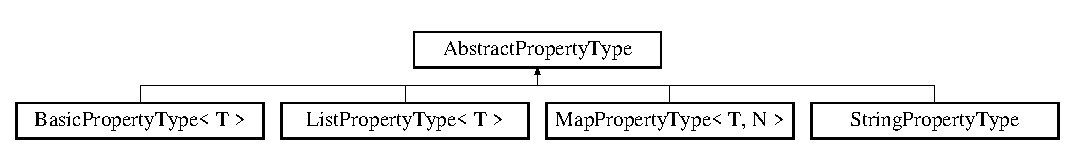
\includegraphics[height=1.637427cm]{classAbstractPropertyType}
\end{center}
\end{figure}
\subsection*{Public Member Functions}
\begin{DoxyCompactItemize}
\item 
\hypertarget{classAbstractPropertyType_a2a525d57a943122e1cc709f738deb13e}{{\bfseries Abstract\-Property\-Type} (std\-::string property)}\label{classAbstractPropertyType_a2a525d57a943122e1cc709f738deb13e}

\item 
\hypertarget{classAbstractPropertyType_a4c359b2e7c3b0ede21c64ba2c90567aa}{virtual std\-::string {\bfseries to\-String} () const =0}\label{classAbstractPropertyType_a4c359b2e7c3b0ede21c64ba2c90567aa}

\item 
\hypertarget{classAbstractPropertyType_a9fae6e2ced72541b5e2bf321a1d193b0}{virtual void {\bfseries from\-String} (std\-::string)=0}\label{classAbstractPropertyType_a9fae6e2ced72541b5e2bf321a1d193b0}

\item 
\hypertarget{classAbstractPropertyType_ae4c8025e310eb06916a28e0341f3356d}{virtual G\-Variant $\ast$ {\bfseries to\-Variant} ()=0}\label{classAbstractPropertyType_ae4c8025e310eb06916a28e0341f3356d}

\item 
\hypertarget{classAbstractPropertyType_a3de5f842aa061f168438e67ca29c2685}{virtual void {\bfseries from\-Variant} (G\-Variant $\ast$)=0}\label{classAbstractPropertyType_a3de5f842aa061f168438e67ca29c2685}

\item 
\hypertarget{classAbstractPropertyType_a8fedd4300acc7ba7ada94e964f2fd166}{virtual \hyperlink{classAbstractPropertyType}{Abstract\-Property\-Type} $\ast$ {\bfseries copy} ()=0}\label{classAbstractPropertyType_a8fedd4300acc7ba7ada94e964f2fd166}

\item 
\hypertarget{classAbstractPropertyType_af156588f45c7b2f2107a8ebb8977e71f}{bool {\bfseries operator==} (\hyperlink{classAbstractPropertyType}{Abstract\-Property\-Type} \&other)}\label{classAbstractPropertyType_af156588f45c7b2f2107a8ebb8977e71f}

\item 
\hypertarget{classAbstractPropertyType_a137d170e61776d59cff141d2df7cab9b}{bool {\bfseries operator!=} (\hyperlink{classAbstractPropertyType}{Abstract\-Property\-Type} \&other)}\label{classAbstractPropertyType_a137d170e61776d59cff141d2df7cab9b}

\item 
\hypertarget{classAbstractPropertyType_ab0de214290dde344d367c7281d293020}{void {\bfseries set\-Value} (boost\-::any val)}\label{classAbstractPropertyType_ab0de214290dde344d367c7281d293020}

\item 
\hypertarget{classAbstractPropertyType_ae723621925382263eba046fa1ca8e36d}{{\footnotesize template$<$typename T $>$ }\\T {\bfseries value} () const }\label{classAbstractPropertyType_ae723621925382263eba046fa1ca8e36d}

\item 
\hypertarget{classAbstractPropertyType_a7ba4118acb746d2b8fc220a12b0e2666}{boost\-::any {\bfseries any\-Value} ()}\label{classAbstractPropertyType_a7ba4118acb746d2b8fc220a12b0e2666}

\end{DoxyCompactItemize}
\subsection*{Public Attributes}
\begin{DoxyCompactItemize}
\item 
\hypertarget{classAbstractPropertyType_a0899de35293963a6c18a0f4913916871}{std\-::string {\bfseries name}}\label{classAbstractPropertyType_a0899de35293963a6c18a0f4913916871}

\item 
\hypertarget{classAbstractPropertyType_a6a391546600fde38a351d3d236be8a9b}{double {\bfseries timestamp}}\label{classAbstractPropertyType_a6a391546600fde38a351d3d236be8a9b}

\item 
\hypertarget{classAbstractPropertyType_ae74440c78c4a5f6af1c3b9c85f1a34c2}{int32\-\_\-t {\bfseries sequence}}\label{classAbstractPropertyType_ae74440c78c4a5f6af1c3b9c85f1a34c2}

\item 
\hypertarget{classAbstractPropertyType_abe2de53722d28e8e7c2a715b97e1ae48}{std\-::string {\bfseries source\-Uuid}}\label{classAbstractPropertyType_abe2de53722d28e8e7c2a715b97e1ae48}

\item 
\hypertarget{classAbstractPropertyType_a420b96a1fcbcbe513ff3801185e788bc}{Zone\-::\-Type {\bfseries zone}}\label{classAbstractPropertyType_a420b96a1fcbcbe513ff3801185e788bc}

\end{DoxyCompactItemize}
\subsection*{Protected Attributes}
\begin{DoxyCompactItemize}
\item 
\hypertarget{classAbstractPropertyType_a69b5d8cd643415d4f63cd6a9e19721d9}{boost\-::any {\bfseries m\-Value}}\label{classAbstractPropertyType_a69b5d8cd643415d4f63cd6a9e19721d9}

\end{DoxyCompactItemize}


The documentation for this class was generated from the following file\-:\begin{DoxyCompactItemize}
\item 
/home/tripzero/src/automotive-\/message-\/broker/lib/abstractpropertytype.\-h\end{DoxyCompactItemize}

\hypertarget{classAbstractRoutingEngine}{\section{Abstract\-Routing\-Engine Class Reference}
\label{classAbstractRoutingEngine}\index{Abstract\-Routing\-Engine@{Abstract\-Routing\-Engine}}
}
\subsection*{Public Types}
\begin{DoxyCompactItemize}
\item 
\hypertarget{classAbstractRoutingEngine_aea584dbb4853b86a3020783bfe9e0608}{typedef std\-::function$<$ void(\hyperlink{classAbstractPropertyType}{Abstract\-Property\-Type} \\*
$\ast$value)$>$ {\bfseries Property\-Changed\-Type}}\label{classAbstractRoutingEngine_aea584dbb4853b86a3020783bfe9e0608}

\end{DoxyCompactItemize}
\subsection*{Public Member Functions}
\begin{DoxyCompactItemize}
\item 
\hypertarget{classAbstractRoutingEngine_ad88ea00def2bb5991f5b2b424acab6c8}{virtual void {\bfseries register\-Source} (\hyperlink{classAbstractSource}{Abstract\-Source} $\ast$src)=0}\label{classAbstractRoutingEngine_ad88ea00def2bb5991f5b2b424acab6c8}

\item 
\hypertarget{classAbstractRoutingEngine_a177588ad6d45f477f596eb025dcc8bed}{virtual void {\bfseries update\-Supported} (Property\-List added, Property\-List removed, \hyperlink{classAbstractSource}{Abstract\-Source} $\ast$source)=0}\label{classAbstractRoutingEngine_a177588ad6d45f477f596eb025dcc8bed}

\item 
\hypertarget{classAbstractRoutingEngine_adadf5f60f3895bdb90bb224d05ee97f0}{void \hyperlink{classAbstractRoutingEngine_adadf5f60f3895bdb90bb224d05ee97f0}{update\-Property} (Vehicle\-Property\-::\-Property property, \hyperlink{classAbstractPropertyType}{Abstract\-Property\-Type} $\ast$value, std\-::string uuid)}\label{classAbstractRoutingEngine_adadf5f60f3895bdb90bb224d05ee97f0}

\begin{DoxyCompactList}\small\item\em Deprecated\-: \end{DoxyCompactList}\item 
\hypertarget{classAbstractRoutingEngine_a2395e520ddfd532959706a5122998fbb}{virtual void {\bfseries update\-Property} (\hyperlink{classAbstractPropertyType}{Abstract\-Property\-Type} $\ast$value, const std\-::string \&uuid)=0}\label{classAbstractRoutingEngine_a2395e520ddfd532959706a5122998fbb}

\item 
\hypertarget{classAbstractRoutingEngine_adcd80e2e3823af7101c5d1f7ff0c217c}{virtual Property\-List {\bfseries supported} ()=0}\label{classAbstractRoutingEngine_adcd80e2e3823af7101c5d1f7ff0c217c}

\item 
\hypertarget{classAbstractRoutingEngine_a179052d9ab3f70ddb4c91421f94c45a9}{virtual void \hyperlink{classAbstractRoutingEngine_a179052d9ab3f70ddb4c91421f94c45a9}{register\-Sink} (\hyperlink{classAbstractSink}{Abstract\-Sink} $\ast$self)=0}\label{classAbstractRoutingEngine_a179052d9ab3f70ddb4c91421f94c45a9}

\begin{DoxyCompactList}\small\item\em sinks\-: \end{DoxyCompactList}\item 
\hypertarget{classAbstractRoutingEngine_a0f0a96c938c395565d01e0f78cc3bea8}{virtual void {\bfseries unregister\-Sink} (\hyperlink{classAbstractSink}{Abstract\-Sink} $\ast$self)=0}\label{classAbstractRoutingEngine_a0f0a96c938c395565d01e0f78cc3bea8}

\item 
virtual std\-::list$<$ std\-::string $>$ \hyperlink{classAbstractRoutingEngine_a9eb81869eaa35dc53f1c0eb6d53f7968}{sources\-For\-Property} (Vehicle\-Property\-::\-Property property)=0
\item 
virtual \hyperlink{classAsyncPropertyReply}{Async\-Property\-Reply} $\ast$ \hyperlink{classAbstractRoutingEngine_ad1cbda415f674be4a3ce49be05aa8ee8}{get\-Property\-Async} (\hyperlink{classAsyncPropertyRequest}{Async\-Property\-Request} request)=0
\item 
\hypertarget{classAbstractRoutingEngine_a335eaf3aea69c5b55b28819119156dd6}{virtual \hyperlink{classAsyncRangePropertyReply}{Async\-Range\-Property\-Reply} $\ast$ {\bfseries get\-Range\-Property\-Async} (\hyperlink{classAsyncRangePropertyRequest}{Async\-Range\-Property\-Request} request)=0}\label{classAbstractRoutingEngine_a335eaf3aea69c5b55b28819119156dd6}

\item 
\hypertarget{classAbstractRoutingEngine_a740b2c9bd8f842499cf250f660553651}{virtual \hyperlink{classAsyncPropertyReply}{Async\-Property\-Reply} $\ast$ {\bfseries set\-Property} (\hyperlink{classAsyncSetPropertyRequest}{Async\-Set\-Property\-Request} request)=0}\label{classAbstractRoutingEngine_a740b2c9bd8f842499cf250f660553651}

\item 
virtual uint \hyperlink{classAbstractRoutingEngine_a1641a8e29180b5faf57ac3bfa3f10cf0}{subscribe\-To\-Property} (Vehicle\-Property\-::\-Property property\-Name, Property\-Changed\-Type callback, std\-::string pid=\char`\"{}\char`\"{})=0
\begin{DoxyCompactList}\small\item\em subscribe\-To\-Property subscribes to property\-Name. Value changes will be passed to callback. \end{DoxyCompactList}\item 
virtual void \hyperlink{classAbstractRoutingEngine_aa56c145aa682ece99791831bc7c420f7}{unsubscribe\-To\-Property} (uint handle)=0
\begin{DoxyCompactList}\small\item\em unsubscribe\-To\-Property \end{DoxyCompactList}\item 
\hypertarget{classAbstractRoutingEngine_ac2690c98fc6d0ccd1fd8cb9b8249644d}{virtual bool {\bfseries subscribe\-To\-Property} (Vehicle\-Property\-::\-Property property\-Name, \hyperlink{classAbstractSink}{Abstract\-Sink} $\ast$self)=0}\label{classAbstractRoutingEngine_ac2690c98fc6d0ccd1fd8cb9b8249644d}

\item 
virtual bool \hyperlink{classAbstractRoutingEngine_a89b4fee7c881662660c530fbcf786648}{subscribe\-To\-Property} (Vehicle\-Property\-::\-Property property\-Name, std\-::string source\-Uuid\-Filter, \hyperlink{classAbstractSink}{Abstract\-Sink} $\ast$self)=0
\begin{DoxyCompactList}\small\item\em subscribe\-To\-Property subscribe to changes made to a property value. \end{DoxyCompactList}\item 
virtual bool \hyperlink{classAbstractRoutingEngine_ae11da6ec0b7438d570c2eb72318c43ee}{subscribe\-To\-Property} (Vehicle\-Property\-::\-Property property\-Name, std\-::string source\-Uuid\-Filter, Zone\-::\-Type zone\-Filter, \hyperlink{classAbstractSink}{Abstract\-Sink} $\ast$self)=0
\begin{DoxyCompactList}\small\item\em subscribe\-To\-Property subscribe to changes made to a property value. \end{DoxyCompactList}\item 
\hypertarget{classAbstractRoutingEngine_afe919effa9d06a8691c34f18774da873}{virtual bool {\bfseries unsubscribe\-To\-Property} (Vehicle\-Property\-::\-Property, \hyperlink{classAbstractSink}{Abstract\-Sink} $\ast$self)=0}\label{classAbstractRoutingEngine_afe919effa9d06a8691c34f18774da873}

\item 
\hypertarget{classAbstractRoutingEngine_a63a98e81d8ebff758f0b7df3325388ae}{virtual \hyperlink{classPropertyInfo}{Property\-Info} {\bfseries get\-Property\-Info} (Vehicle\-Property\-::\-Property, std\-::string source\-Uuid)=0}\label{classAbstractRoutingEngine_a63a98e81d8ebff758f0b7df3325388ae}

\end{DoxyCompactItemize}


\subsection{Member Function Documentation}
\hypertarget{classAbstractRoutingEngine_ad1cbda415f674be4a3ce49be05aa8ee8}{\index{Abstract\-Routing\-Engine@{Abstract\-Routing\-Engine}!get\-Property\-Async@{get\-Property\-Async}}
\index{get\-Property\-Async@{get\-Property\-Async}!AbstractRoutingEngine@{Abstract\-Routing\-Engine}}
\subsubsection[{get\-Property\-Async}]{\setlength{\rightskip}{0pt plus 5cm}virtual {\bf Async\-Property\-Reply}$\ast$ Abstract\-Routing\-Engine\-::get\-Property\-Async (
\begin{DoxyParamCaption}
\item[{{\bf Async\-Property\-Request}}]{request}
\end{DoxyParamCaption}
)\hspace{0.3cm}{\ttfamily [pure virtual]}}}\label{classAbstractRoutingEngine_ad1cbda415f674be4a3ce49be05aa8ee8}
/brief get\-Property\-Async requests a property value from a source. This call has a timeout and the callback specified in the request will always be called. /see \hyperlink{classAsyncPropertyRequest}{Async\-Property\-Request} /see \hyperlink{classAsyncPropertyReply}{Async\-Property\-Reply}. /param request requested property. /return \hyperlink{classAsyncPropertyReply}{Async\-Property\-Reply}. The returned \hyperlink{classAsyncPropertyReply}{Async\-Property\-Reply} is owned by the caller of get\-Property\-Async. /example \hyperlink{classAsyncPropertyRequest}{Async\-Property\-Request} request; request.\-property = Vehicle\-Property\-::\-Vehicle\-Speed request.\-completed = \mbox{[}\mbox{]}(Async\-Property\-Reply$\ast$ reply) \{ //you own the reply delete reply; \}; routing\-Engine-\/$>$get\-Property\-Async(request); \hypertarget{classAbstractRoutingEngine_a9eb81869eaa35dc53f1c0eb6d53f7968}{\index{Abstract\-Routing\-Engine@{Abstract\-Routing\-Engine}!sources\-For\-Property@{sources\-For\-Property}}
\index{sources\-For\-Property@{sources\-For\-Property}!AbstractRoutingEngine@{Abstract\-Routing\-Engine}}
\subsubsection[{sources\-For\-Property}]{\setlength{\rightskip}{0pt plus 5cm}virtual std\-::list$<$std\-::string$>$ Abstract\-Routing\-Engine\-::sources\-For\-Property (
\begin{DoxyParamCaption}
\item[{Vehicle\-Property\-::\-Property}]{property}
\end{DoxyParamCaption}
)\hspace{0.3cm}{\ttfamily [pure virtual]}}}\label{classAbstractRoutingEngine_a9eb81869eaa35dc53f1c0eb6d53f7968}
/brief sources\-For\-Property /param property /return list of source uuid's that support the \char`\"{}property\char`\"{} \hypertarget{classAbstractRoutingEngine_a1641a8e29180b5faf57ac3bfa3f10cf0}{\index{Abstract\-Routing\-Engine@{Abstract\-Routing\-Engine}!subscribe\-To\-Property@{subscribe\-To\-Property}}
\index{subscribe\-To\-Property@{subscribe\-To\-Property}!AbstractRoutingEngine@{Abstract\-Routing\-Engine}}
\subsubsection[{subscribe\-To\-Property}]{\setlength{\rightskip}{0pt plus 5cm}virtual uint Abstract\-Routing\-Engine\-::subscribe\-To\-Property (
\begin{DoxyParamCaption}
\item[{Vehicle\-Property\-::\-Property}]{property\-Name, }
\item[{Property\-Changed\-Type}]{callback, }
\item[{std\-::string}]{pid = {\ttfamily \char`\"{}\char`\"{}}}
\end{DoxyParamCaption}
)\hspace{0.3cm}{\ttfamily [pure virtual]}}}\label{classAbstractRoutingEngine_a1641a8e29180b5faf57ac3bfa3f10cf0}


subscribe\-To\-Property subscribes to property\-Name. Value changes will be passed to callback. 


\begin{DoxyParams}{Parameters}
{\em property\-Name} & \\
\hline
{\em callback} & \\
\hline
{\em pid} & process id of the requesting application \\
\hline
\end{DoxyParams}
\begin{DoxyReturn}{Returns}
subscription handle 
\end{DoxyReturn}
\hypertarget{classAbstractRoutingEngine_a89b4fee7c881662660c530fbcf786648}{\index{Abstract\-Routing\-Engine@{Abstract\-Routing\-Engine}!subscribe\-To\-Property@{subscribe\-To\-Property}}
\index{subscribe\-To\-Property@{subscribe\-To\-Property}!AbstractRoutingEngine@{Abstract\-Routing\-Engine}}
\subsubsection[{subscribe\-To\-Property}]{\setlength{\rightskip}{0pt plus 5cm}virtual bool Abstract\-Routing\-Engine\-::subscribe\-To\-Property (
\begin{DoxyParamCaption}
\item[{Vehicle\-Property\-::\-Property}]{property\-Name, }
\item[{std\-::string}]{source\-Uuid\-Filter, }
\item[{{\bf Abstract\-Sink} $\ast$}]{self}
\end{DoxyParamCaption}
)\hspace{0.3cm}{\ttfamily [pure virtual]}}}\label{classAbstractRoutingEngine_a89b4fee7c881662660c530fbcf786648}


subscribe\-To\-Property subscribe to changes made to a property value. 


\begin{DoxyParams}{Parameters}
{\em property\-Name} & name of the property to request a subscription for. \\
\hline
{\em source\-Uuid\-Filter} & source U\-U\-I\-D to filter. Only property updates from this source will be sent to the sink. \\
\hline
{\em self} & pointer to the sink who is subscribing. \\
\hline
\end{DoxyParams}
\hypertarget{classAbstractRoutingEngine_ae11da6ec0b7438d570c2eb72318c43ee}{\index{Abstract\-Routing\-Engine@{Abstract\-Routing\-Engine}!subscribe\-To\-Property@{subscribe\-To\-Property}}
\index{subscribe\-To\-Property@{subscribe\-To\-Property}!AbstractRoutingEngine@{Abstract\-Routing\-Engine}}
\subsubsection[{subscribe\-To\-Property}]{\setlength{\rightskip}{0pt plus 5cm}virtual bool Abstract\-Routing\-Engine\-::subscribe\-To\-Property (
\begin{DoxyParamCaption}
\item[{Vehicle\-Property\-::\-Property}]{property\-Name, }
\item[{std\-::string}]{source\-Uuid\-Filter, }
\item[{Zone\-::\-Type}]{zone\-Filter, }
\item[{{\bf Abstract\-Sink} $\ast$}]{self}
\end{DoxyParamCaption}
)\hspace{0.3cm}{\ttfamily [pure virtual]}}}\label{classAbstractRoutingEngine_ae11da6ec0b7438d570c2eb72318c43ee}


subscribe\-To\-Property subscribe to changes made to a property value. 


\begin{DoxyParams}{Parameters}
{\em property\-Name} & name of the property to request a subscription for. \\
\hline
{\em source\-Uuid\-Filter} & source U\-U\-I\-D to filter. Only property updates from this source will be sent to the sink. \\
\hline
{\em zone\-Filter} & zone to filter. Only updates from this zone will be passed to the sink. \\
\hline
{\em self} & pointer to the sink who is subscribing. \\
\hline
\end{DoxyParams}
\hypertarget{classAbstractRoutingEngine_aa56c145aa682ece99791831bc7c420f7}{\index{Abstract\-Routing\-Engine@{Abstract\-Routing\-Engine}!unsubscribe\-To\-Property@{unsubscribe\-To\-Property}}
\index{unsubscribe\-To\-Property@{unsubscribe\-To\-Property}!AbstractRoutingEngine@{Abstract\-Routing\-Engine}}
\subsubsection[{unsubscribe\-To\-Property}]{\setlength{\rightskip}{0pt plus 5cm}virtual void Abstract\-Routing\-Engine\-::unsubscribe\-To\-Property (
\begin{DoxyParamCaption}
\item[{uint}]{handle}
\end{DoxyParamCaption}
)\hspace{0.3cm}{\ttfamily [pure virtual]}}}\label{classAbstractRoutingEngine_aa56c145aa682ece99791831bc7c420f7}


unsubscribe\-To\-Property 


\begin{DoxyParams}{Parameters}
{\em handle} & \\
\hline
\end{DoxyParams}


The documentation for this class was generated from the following files\-:\begin{DoxyCompactItemize}
\item 
/home/kev/src/automotive-\/message-\/broker/lib/abstractroutingengine.\-h\item 
/home/kev/src/automotive-\/message-\/broker/lib/abstractroutingengine.\-cpp\end{DoxyCompactItemize}

\hypertarget{classAbstractSink}{\section{Abstract\-Sink Class Reference}
\label{classAbstractSink}\index{Abstract\-Sink@{Abstract\-Sink}}
}
Inheritance diagram for Abstract\-Sink\-:\begin{figure}[H]
\begin{center}
\leavevmode
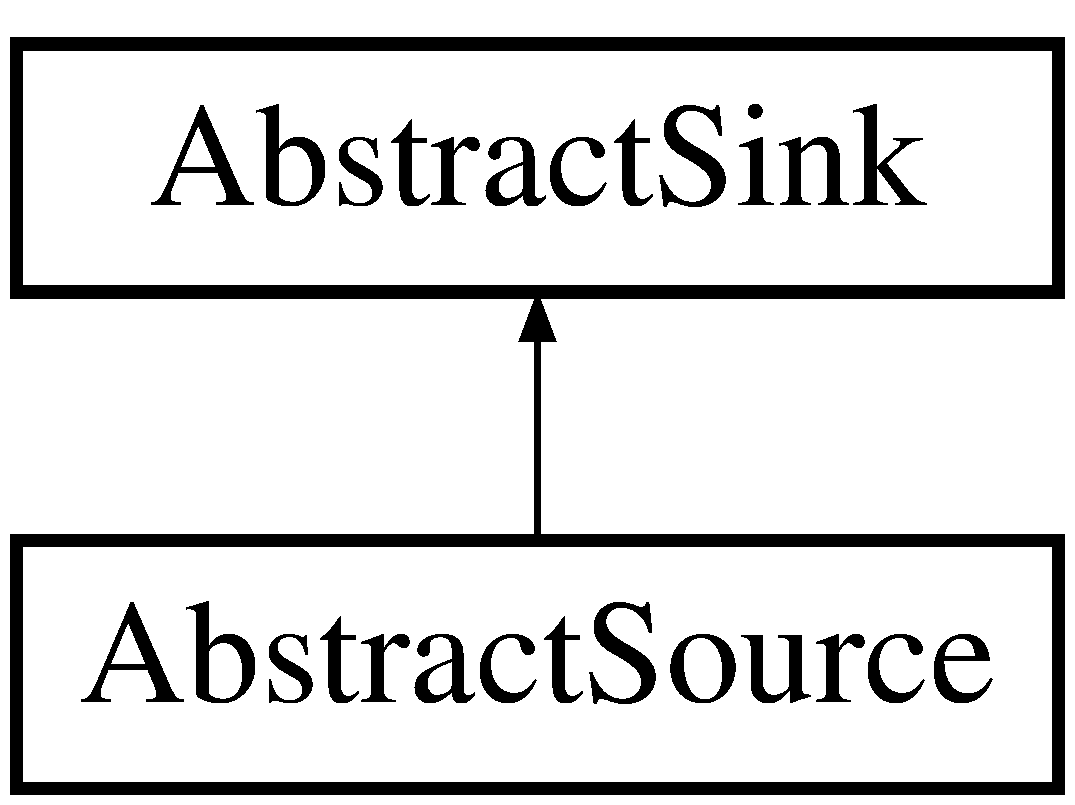
\includegraphics[height=2.000000cm]{classAbstractSink}
\end{center}
\end{figure}
\subsection*{Public Member Functions}
\begin{DoxyCompactItemize}
\item 
\hypertarget{classAbstractSink_a63f03d63fd091cd6f39a9888dd08ea6a}{{\bfseries Abstract\-Sink} (\hyperlink{classAbstractRoutingEngine}{Abstract\-Routing\-Engine} $\ast$engine, map$<$ string, string $>$ config)}\label{classAbstractSink_a63f03d63fd091cd6f39a9888dd08ea6a}

\item 
virtual const string \hyperlink{classAbstractSink_a965ae1d5218713c7823fbd95fa51b053}{uuid} ()=0
\begin{DoxyCompactList}\small\item\em Pure virtual methods\-: \end{DoxyCompactList}\item 
virtual void \hyperlink{classAbstractSink_afeb683c566a5a71303d05d2e12da2b28}{property\-Changed} (\hyperlink{classAbstractPropertyType}{Abstract\-Property\-Type} $\ast$value)
\begin{DoxyCompactList}\small\item\em property\-Changed is called when a subscribed to property changes. \end{DoxyCompactList}\item 
virtual void \hyperlink{classAbstractSink_aec23151301927f57330022beb175527b}{supported\-Changed} (Property\-List supported\-Properties)=0
\end{DoxyCompactItemize}
\subsection*{Protected Attributes}
\begin{DoxyCompactItemize}
\item 
\hypertarget{classAbstractSink_a4d49a722e60cd9993c182a29fbf74591}{\hyperlink{classAbstractRoutingEngine}{Abstract\-Routing\-Engine} $\ast$ \hyperlink{classAbstractSink_a4d49a722e60cd9993c182a29fbf74591}{routing\-Engine}}\label{classAbstractSink_a4d49a722e60cd9993c182a29fbf74591}

\begin{DoxyCompactList}\small\item\em routing\-Engine is the core of A\-M\-B. It is used to pass plugin and property information to other plugins \end{DoxyCompactList}\item 
\hypertarget{classAbstractSink_a52581d514cad8b74a9fb42a026522f76}{map$<$ string, string $>$ {\bfseries configuration}}\label{classAbstractSink_a52581d514cad8b74a9fb42a026522f76}

\end{DoxyCompactItemize}


\subsection{Member Function Documentation}
\hypertarget{classAbstractSink_afeb683c566a5a71303d05d2e12da2b28}{\index{Abstract\-Sink@{Abstract\-Sink}!property\-Changed@{property\-Changed}}
\index{property\-Changed@{property\-Changed}!AbstractSink@{Abstract\-Sink}}
\subsubsection[{property\-Changed}]{\setlength{\rightskip}{0pt plus 5cm}virtual void Abstract\-Sink\-::property\-Changed (
\begin{DoxyParamCaption}
\item[{{\bf Abstract\-Property\-Type} $\ast$}]{value}
\end{DoxyParamCaption}
)\hspace{0.3cm}{\ttfamily [inline]}, {\ttfamily [virtual]}}}\label{classAbstractSink_afeb683c566a5a71303d05d2e12da2b28}


property\-Changed is called when a subscribed to property changes. 

\begin{DoxySeeAlso}{See Also}
Abstract\-Routing\-Engine\-::subscribe\-To\-Property\-Changes() 
\end{DoxySeeAlso}

\begin{DoxyParams}{Parameters}
{\em value} & value of the property that changed. this is a temporary pointer that will be destroyed. Do not destroy it. If you need to store the value use value.\-any\-Value(), value.\-value$<$\-T$>$() or value-\/$>$copy() to copy. \\
\hline
\end{DoxyParams}
\hypertarget{classAbstractSink_aec23151301927f57330022beb175527b}{\index{Abstract\-Sink@{Abstract\-Sink}!supported\-Changed@{supported\-Changed}}
\index{supported\-Changed@{supported\-Changed}!AbstractSink@{Abstract\-Sink}}
\subsubsection[{supported\-Changed}]{\setlength{\rightskip}{0pt plus 5cm}virtual void Abstract\-Sink\-::supported\-Changed (
\begin{DoxyParamCaption}
\item[{Property\-List}]{supported\-Properties}
\end{DoxyParamCaption}
)\hspace{0.3cm}{\ttfamily [pure virtual]}}}\label{classAbstractSink_aec23151301927f57330022beb175527b}
\hyperlink{classAbstractSink_aec23151301927f57330022beb175527b}{supported\-Changed()} is called when the supported properties changes \begin{DoxyItemize}
\item supported\-Properties the new list of supported properties. \end{DoxyItemize}
\hypertarget{classAbstractSink_a965ae1d5218713c7823fbd95fa51b053}{\index{Abstract\-Sink@{Abstract\-Sink}!uuid@{uuid}}
\index{uuid@{uuid}!AbstractSink@{Abstract\-Sink}}
\subsubsection[{uuid}]{\setlength{\rightskip}{0pt plus 5cm}virtual const string Abstract\-Sink\-::uuid (
\begin{DoxyParamCaption}
{}
\end{DoxyParamCaption}
)\hspace{0.3cm}{\ttfamily [pure virtual]}}}\label{classAbstractSink_a965ae1d5218713c7823fbd95fa51b053}


Pure virtual methods\-: 

\hyperlink{classAbstractSink_a965ae1d5218713c7823fbd95fa51b053}{uuid()} is a unique identifier \begin{DoxyReturn}{Returns}
a guid-\/style unique identifier 
\end{DoxyReturn}


The documentation for this class was generated from the following files\-:\begin{DoxyCompactItemize}
\item 
/home/tripzero/src/automotive-\/message-\/broker/lib/abstractsink.\-h\item 
/home/tripzero/src/automotive-\/message-\/broker/lib/abstractsink.\-cpp\end{DoxyCompactItemize}

\hypertarget{classAbstractSinkManager}{\section{Abstract\-Sink\-Manager Class Reference}
\label{classAbstractSinkManager}\index{Abstract\-Sink\-Manager@{Abstract\-Sink\-Manager}}
}


T\-O\-D\-O\-: this class actually serves no purpose.  




{\ttfamily \#include $<$abstractsink.\-h$>$}

\subsection*{Public Member Functions}
\begin{DoxyCompactItemize}
\item 
\hypertarget{classAbstractSinkManager_a8c2b065455e7392bbef66056e492cf54}{{\bfseries Abstract\-Sink\-Manager} (\hyperlink{classAbstractRoutingEngine}{Abstract\-Routing\-Engine} $\ast$engine, map$<$ string, string $>$ config)}\label{classAbstractSinkManager_a8c2b065455e7392bbef66056e492cf54}

\end{DoxyCompactItemize}
\subsection*{Protected Attributes}
\begin{DoxyCompactItemize}
\item 
\hypertarget{classAbstractSinkManager_aa4951761c33e7012c3a0e72e099354b3}{\hyperlink{classAbstractRoutingEngine}{Abstract\-Routing\-Engine} $\ast$ {\bfseries routing\-Engine}}\label{classAbstractSinkManager_aa4951761c33e7012c3a0e72e099354b3}

\item 
\hypertarget{classAbstractSinkManager_ac329710da75b1c757584ec42a8072ea4}{map$<$ string, string $>$ {\bfseries configuration}}\label{classAbstractSinkManager_ac329710da75b1c757584ec42a8072ea4}

\end{DoxyCompactItemize}


\subsection{Detailed Description}
T\-O\-D\-O\-: this class actually serves no purpose. 

The documentation for this class was generated from the following files\-:\begin{DoxyCompactItemize}
\item 
/home/tripzero/src/automotive-\/message-\/broker/lib/abstractsink.\-h\item 
/home/tripzero/src/automotive-\/message-\/broker/lib/abstractsink.\-cpp\end{DoxyCompactItemize}

\hypertarget{classAbstractSource}{\section{Abstract\-Source Class Reference}
\label{classAbstractSource}\index{Abstract\-Source@{Abstract\-Source}}
}
Inheritance diagram for Abstract\-Source\-:\begin{figure}[H]
\begin{center}
\leavevmode
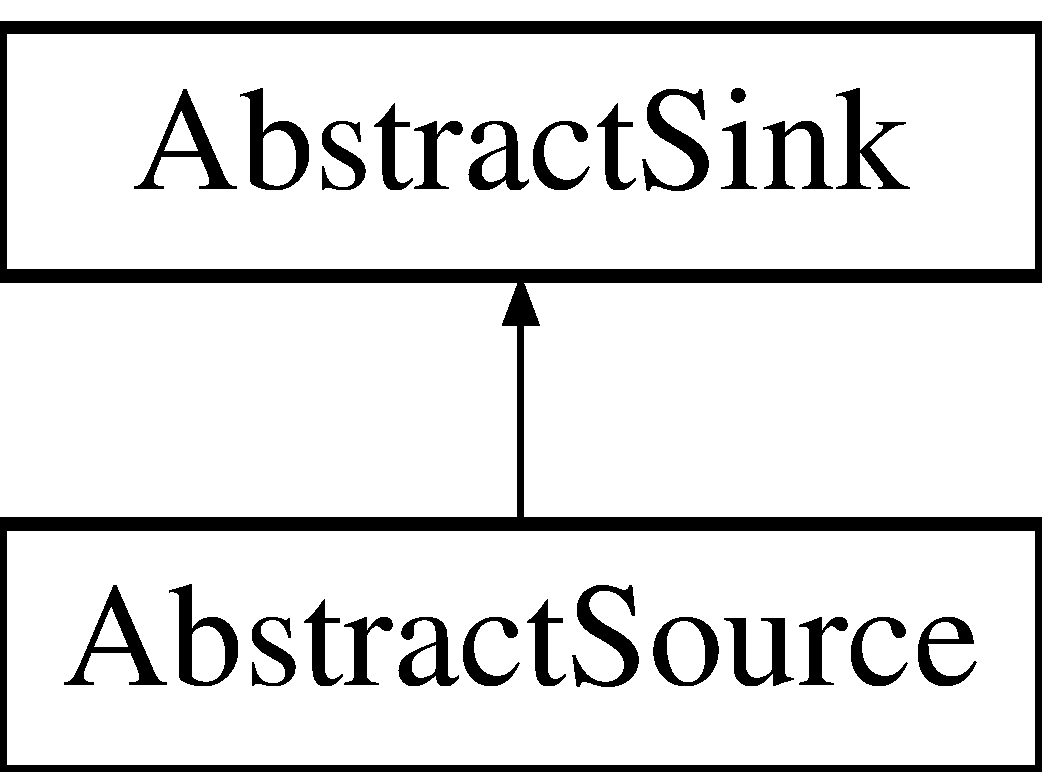
\includegraphics[height=2.000000cm]{classAbstractSource}
\end{center}
\end{figure}
\subsection*{Public Types}
\begin{DoxyCompactItemize}
\item 
enum \hyperlink{classAbstractSource_aad1e5e4914f2aa174dfd8fa6e143c1b9}{Operations} \{ {\bfseries Get} = 0x01, 
{\bfseries Set} = 0x02, 
{\bfseries Get\-Ranged} = 0x04
 \}
\begin{DoxyCompactList}\small\item\em The Operations enum is a bitmask flag used to specify which operations are supported by the source plugin. \end{DoxyCompactList}\end{DoxyCompactItemize}
\subsection*{Public Member Functions}
\begin{DoxyCompactItemize}
\item 
\hypertarget{classAbstractSource_a753c78f3ee4c565c4ba2157c06cb7fbe}{{\bfseries Abstract\-Source} (\hyperlink{classAbstractRoutingEngine}{Abstract\-Routing\-Engine} $\ast$engine, map$<$ string, string $>$ config)}\label{classAbstractSource_a753c78f3ee4c565c4ba2157c06cb7fbe}

\item 
virtual void \hyperlink{classAbstractSource_a05589e699ea16a14675db226d51bdf9f}{get\-Property\-Async} (\hyperlink{classAsyncPropertyReply}{Async\-Property\-Reply} $\ast$reply)=0
\begin{DoxyCompactList}\small\item\em pure virtual methods\-: \end{DoxyCompactList}\item 
virtual void \hyperlink{classAbstractSource_a3b30f939d68889b2540f6035fa5be7c7}{get\-Range\-Property\-Async} (\hyperlink{classAsyncRangePropertyReply}{Async\-Range\-Property\-Reply} $\ast$reply)=0
\begin{DoxyCompactList}\small\item\em get\-Range\-Property\-Async is called when a sink requests a series of values for a given property within a specified time or sequencial range. This will only be called if the source support the Ranged Operation ( \end{DoxyCompactList}\item 
virtual \hyperlink{classAsyncPropertyReply}{Async\-Property\-Reply} $\ast$ \hyperlink{classAbstractSource_a684b58112b5572dfe8cb94380bf7d74a}{set\-Property} (\hyperlink{classAsyncSetPropertyRequest}{Async\-Set\-Property\-Request} request)=0
\begin{DoxyCompactList}\small\item\em set\-Property is called when a sink requests to set a value for a given property. This is only called if the source supports the Set Operation ( \end{DoxyCompactList}\item 
virtual void \hyperlink{classAbstractSource_ae9c042e159f080c298b2ae37c47618e9}{subscribe\-To\-Property\-Changes} (Vehicle\-Property\-::\-Property property)=0
\begin{DoxyCompactList}\small\item\em subscribe\-To\-Property\-Changes is called when a sink requests a subscription. Source plugins can keep track of subscriptions and may wish to sleep if there are no subscriptions. \end{DoxyCompactList}\item 
virtual void \hyperlink{classAbstractSource_a584372310f191b1b9067a634b7366023}{unsubscribe\-To\-Property\-Changes} (Vehicle\-Property\-::\-Property property)=0
\begin{DoxyCompactList}\small\item\em unsubscribe\-To\-Property\-Changes is called when a sink requests to unsubscribe from a given property's changes. \end{DoxyCompactList}\item 
virtual Property\-List \hyperlink{classAbstractSource_ad8330cbbac84dc24851eb50ff7243460}{supported} ()=0
\begin{DoxyCompactList}\small\item\em supported is called by the routing\-Engine ( \end{DoxyCompactList}\item 
virtual int \hyperlink{classAbstractSource_a317861675652372a72fc01c075036b51}{supported\-Operations} ()=0
\begin{DoxyCompactList}\small\item\em supported\-Operations \end{DoxyCompactList}\item 
virtual \hyperlink{classPropertyInfo}{Property\-Info} \hyperlink{classAbstractSource_a5818ef06a4610d4969c6e1ed6a0c6242}{get\-Property\-Info} (Vehicle\-Property\-::\-Property property)
\begin{DoxyCompactList}\small\item\em get\-Property\-Info used to return specific information about a property \end{DoxyCompactList}\end{DoxyCompactItemize}
\subsection*{Protected Attributes}
\begin{DoxyCompactItemize}
\item 
\hyperlink{classAbstractRoutingEngine}{Abstract\-Routing\-Engine} $\ast$ \hyperlink{classAbstractSource_aabbce93fea123c54be55a007c928a6f1}{routing\-Engine}
\begin{DoxyCompactList}\small\item\em routing\-Engine the core routing engine used to send property updates to sink plugins. \end{DoxyCompactList}\end{DoxyCompactItemize}


\subsection{Member Function Documentation}
\hypertarget{classAbstractSource_a05589e699ea16a14675db226d51bdf9f}{\index{Abstract\-Source@{Abstract\-Source}!get\-Property\-Async@{get\-Property\-Async}}
\index{get\-Property\-Async@{get\-Property\-Async}!AbstractSource@{Abstract\-Source}}
\subsubsection[{get\-Property\-Async}]{\setlength{\rightskip}{0pt plus 5cm}virtual void Abstract\-Source\-::get\-Property\-Async (
\begin{DoxyParamCaption}
\item[{{\bf Async\-Property\-Reply} $\ast$}]{reply}
\end{DoxyParamCaption}
)\hspace{0.3cm}{\ttfamily [pure virtual]}}}\label{classAbstractSource_a05589e699ea16a14675db226d51bdf9f}


pure virtual methods\-: 

get\-Property\-Async is called when a sink requests the value for given property. This is only called if the source supports the Get operation (\begin{DoxySeeAlso}{See Also}
Operation) 
\end{DoxySeeAlso}

\begin{DoxyParams}{Parameters}
{\em reply} & the reply variable.\\
\hline
\end{DoxyParams}
\begin{DoxySeeAlso}{See Also}
\hyperlink{classAsyncPropertyReply}{Async\-Property\-Reply} 
\end{DoxySeeAlso}
\hypertarget{classAbstractSource_a5818ef06a4610d4969c6e1ed6a0c6242}{\index{Abstract\-Source@{Abstract\-Source}!get\-Property\-Info@{get\-Property\-Info}}
\index{get\-Property\-Info@{get\-Property\-Info}!AbstractSource@{Abstract\-Source}}
\subsubsection[{get\-Property\-Info}]{\setlength{\rightskip}{0pt plus 5cm}{\bf Property\-Info} Abstract\-Source\-::get\-Property\-Info (
\begin{DoxyParamCaption}
\item[{Vehicle\-Property\-::\-Property}]{property}
\end{DoxyParamCaption}
)\hspace{0.3cm}{\ttfamily [virtual]}}}\label{classAbstractSource_a5818ef06a4610d4969c6e1ed6a0c6242}


get\-Property\-Info used to return specific information about a property 

\begin{DoxySeeAlso}{See Also}
\hyperlink{classPropertyInfo}{Property\-Info} the source should override this otherwise a \hyperlink{classPropertyInfo_a5a3e9a1198ac54a40b1f3ae009bb1397}{Property\-Info\-::invalid()} will be returned for the property 
\end{DoxySeeAlso}

\begin{DoxyParams}{Parameters}
{\em property} & the property to get info for. \\
\hline
\end{DoxyParams}
\begin{DoxyReturn}{Returns}
a \hyperlink{classPropertyInfo}{Property\-Info} object. 
\end{DoxyReturn}
\hypertarget{classAbstractSource_a3b30f939d68889b2540f6035fa5be7c7}{\index{Abstract\-Source@{Abstract\-Source}!get\-Range\-Property\-Async@{get\-Range\-Property\-Async}}
\index{get\-Range\-Property\-Async@{get\-Range\-Property\-Async}!AbstractSource@{Abstract\-Source}}
\subsubsection[{get\-Range\-Property\-Async}]{\setlength{\rightskip}{0pt plus 5cm}virtual void Abstract\-Source\-::get\-Range\-Property\-Async (
\begin{DoxyParamCaption}
\item[{{\bf Async\-Range\-Property\-Reply} $\ast$}]{reply}
\end{DoxyParamCaption}
)\hspace{0.3cm}{\ttfamily [pure virtual]}}}\label{classAbstractSource_a3b30f939d68889b2540f6035fa5be7c7}


get\-Range\-Property\-Async is called when a sink requests a series of values for a given property within a specified time or sequencial range. This will only be called if the source support the Ranged Operation ( 

\begin{DoxySeeAlso}{See Also}
\hyperlink{classAbstractSource_aad1e5e4914f2aa174dfd8fa6e143c1b9}{Operations}) 
\end{DoxySeeAlso}

\begin{DoxyParams}{Parameters}
{\em reply} & is the reply variable.\\
\hline
\end{DoxyParams}
\begin{DoxySeeAlso}{See Also}
\hyperlink{classAsyncRangePropertyReply}{Async\-Range\-Property\-Reply} 
\end{DoxySeeAlso}
\hypertarget{classAbstractSource_a684b58112b5572dfe8cb94380bf7d74a}{\index{Abstract\-Source@{Abstract\-Source}!set\-Property@{set\-Property}}
\index{set\-Property@{set\-Property}!AbstractSource@{Abstract\-Source}}
\subsubsection[{set\-Property}]{\setlength{\rightskip}{0pt plus 5cm}virtual {\bf Async\-Property\-Reply}$\ast$ Abstract\-Source\-::set\-Property (
\begin{DoxyParamCaption}
\item[{{\bf Async\-Set\-Property\-Request}}]{request}
\end{DoxyParamCaption}
)\hspace{0.3cm}{\ttfamily [pure virtual]}}}\label{classAbstractSource_a684b58112b5572dfe8cb94380bf7d74a}


set\-Property is called when a sink requests to set a value for a given property. This is only called if the source supports the Set Operation ( 

\begin{DoxySeeAlso}{See Also}
Operation) 
\end{DoxySeeAlso}

\begin{DoxyParams}{Parameters}
{\em request} & the requested property to set. \\
\hline
\end{DoxyParams}
\begin{DoxyReturn}{Returns}
returns a pointer to the new value for the property.
\end{DoxyReturn}
\begin{DoxySeeAlso}{See Also}
\hyperlink{classAsyncPropertyReply}{Async\-Property\-Reply} 
\end{DoxySeeAlso}
\hypertarget{classAbstractSource_ae9c042e159f080c298b2ae37c47618e9}{\index{Abstract\-Source@{Abstract\-Source}!subscribe\-To\-Property\-Changes@{subscribe\-To\-Property\-Changes}}
\index{subscribe\-To\-Property\-Changes@{subscribe\-To\-Property\-Changes}!AbstractSource@{Abstract\-Source}}
\subsubsection[{subscribe\-To\-Property\-Changes}]{\setlength{\rightskip}{0pt plus 5cm}virtual void Abstract\-Source\-::subscribe\-To\-Property\-Changes (
\begin{DoxyParamCaption}
\item[{Vehicle\-Property\-::\-Property}]{property}
\end{DoxyParamCaption}
)\hspace{0.3cm}{\ttfamily [pure virtual]}}}\label{classAbstractSource_ae9c042e159f080c298b2ae37c47618e9}


subscribe\-To\-Property\-Changes is called when a sink requests a subscription. Source plugins can keep track of subscriptions and may wish to sleep if there are no subscriptions. 


\begin{DoxyParams}{Parameters}
{\em property} & the property that is being subscribed. \\
\hline
\end{DoxyParams}
\begin{DoxySeeAlso}{See Also}
\hyperlink{classAbstractSource_a584372310f191b1b9067a634b7366023}{unsubscribe\-To\-Property\-Changes} 
\end{DoxySeeAlso}
\hypertarget{classAbstractSource_ad8330cbbac84dc24851eb50ff7243460}{\index{Abstract\-Source@{Abstract\-Source}!supported@{supported}}
\index{supported@{supported}!AbstractSource@{Abstract\-Source}}
\subsubsection[{supported}]{\setlength{\rightskip}{0pt plus 5cm}virtual Property\-List Abstract\-Source\-::supported (
\begin{DoxyParamCaption}
{}
\end{DoxyParamCaption}
)\hspace{0.3cm}{\ttfamily [pure virtual]}}}\label{classAbstractSource_ad8330cbbac84dc24851eb50ff7243460}


supported is called by the routing\-Engine ( 

\begin{DoxySeeAlso}{See Also}
\hyperlink{classAbstractRoutingEngine}{Abstract\-Routing\-Engine}) to understand what properties this source supports 
\end{DoxySeeAlso}
\begin{DoxyReturn}{Returns}
returns a list of supported properties. If the the supported properties changed, the source should call Abstract\-Routing\-Engine\-::set\-Supported. 
\end{DoxyReturn}
\hypertarget{classAbstractSource_a317861675652372a72fc01c075036b51}{\index{Abstract\-Source@{Abstract\-Source}!supported\-Operations@{supported\-Operations}}
\index{supported\-Operations@{supported\-Operations}!AbstractSource@{Abstract\-Source}}
\subsubsection[{supported\-Operations}]{\setlength{\rightskip}{0pt plus 5cm}virtual int Abstract\-Source\-::supported\-Operations (
\begin{DoxyParamCaption}
{}
\end{DoxyParamCaption}
)\hspace{0.3cm}{\ttfamily [pure virtual]}}}\label{classAbstractSource_a317861675652372a72fc01c075036b51}


supported\-Operations 

\begin{DoxyReturn}{Returns}
returns the supported operations.
\end{DoxyReturn}
\begin{DoxySeeAlso}{See Also}
\hyperlink{classAbstractSource_aad1e5e4914f2aa174dfd8fa6e143c1b9}{Operations} 
\end{DoxySeeAlso}
\hypertarget{classAbstractSource_a584372310f191b1b9067a634b7366023}{\index{Abstract\-Source@{Abstract\-Source}!unsubscribe\-To\-Property\-Changes@{unsubscribe\-To\-Property\-Changes}}
\index{unsubscribe\-To\-Property\-Changes@{unsubscribe\-To\-Property\-Changes}!AbstractSource@{Abstract\-Source}}
\subsubsection[{unsubscribe\-To\-Property\-Changes}]{\setlength{\rightskip}{0pt plus 5cm}virtual void Abstract\-Source\-::unsubscribe\-To\-Property\-Changes (
\begin{DoxyParamCaption}
\item[{Vehicle\-Property\-::\-Property}]{property}
\end{DoxyParamCaption}
)\hspace{0.3cm}{\ttfamily [pure virtual]}}}\label{classAbstractSource_a584372310f191b1b9067a634b7366023}


unsubscribe\-To\-Property\-Changes is called when a sink requests to unsubscribe from a given property's changes. 


\begin{DoxyParams}{Parameters}
{\em property} & the property to unsubscribe to \\
\hline
\end{DoxyParams}
\begin{DoxySeeAlso}{See Also}
\hyperlink{classAbstractSource_ae9c042e159f080c298b2ae37c47618e9}{subscribe\-To\-Property\-Changes} 
\end{DoxySeeAlso}


\subsection{Member Data Documentation}
\hypertarget{classAbstractSource_aabbce93fea123c54be55a007c928a6f1}{\index{Abstract\-Source@{Abstract\-Source}!routing\-Engine@{routing\-Engine}}
\index{routing\-Engine@{routing\-Engine}!AbstractSource@{Abstract\-Source}}
\subsubsection[{routing\-Engine}]{\setlength{\rightskip}{0pt plus 5cm}{\bf Abstract\-Routing\-Engine}$\ast$ Abstract\-Source\-::routing\-Engine\hspace{0.3cm}{\ttfamily [protected]}}}\label{classAbstractSource_aabbce93fea123c54be55a007c928a6f1}


routing\-Engine the core routing engine used to send property updates to sink plugins. 

\begin{DoxySeeAlso}{See Also}
\hyperlink{classAbstractRoutingEngine}{Abstract\-Routing\-Engine} 
\end{DoxySeeAlso}


The documentation for this class was generated from the following files\-:\begin{DoxyCompactItemize}
\item 
/home/tripzero/src/automotive-\/message-\/broker/lib/abstractsource.\-h\item 
/home/tripzero/src/automotive-\/message-\/broker/lib/abstractsource.\-cpp\end{DoxyCompactItemize}

\hypertarget{classAsyncPropertyReply}{\section{Async\-Property\-Reply Class Reference}
\label{classAsyncPropertyReply}\index{Async\-Property\-Reply@{Async\-Property\-Reply}}
}


The \hyperlink{classAsyncPropertyReply}{Async\-Property\-Reply} class is used by sources to reply to Get and Set operations. The source should set success to true if the call is successful or 'false' if the request was not successful and set 'error' to the appropriate error.  




{\ttfamily \#include $<$abstractroutingengine.\-h$>$}

Inheritance diagram for Async\-Property\-Reply\-:\begin{figure}[H]
\begin{center}
\leavevmode
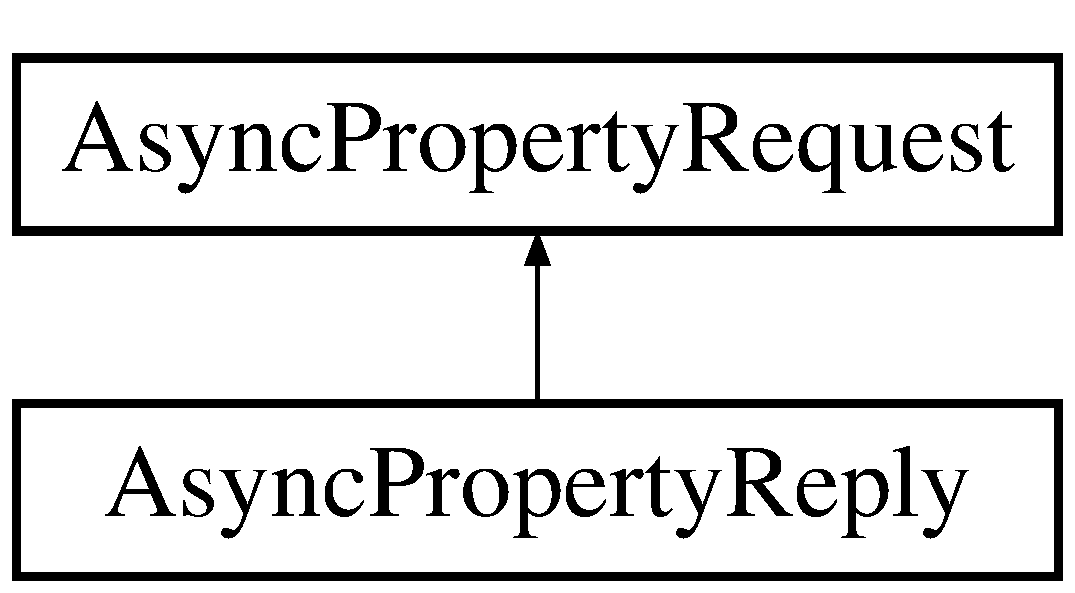
\includegraphics[height=2.000000cm]{classAsyncPropertyReply}
\end{center}
\end{figure}
\subsection*{Public Types}
\begin{DoxyCompactItemize}
\item 
enum \hyperlink{classAsyncPropertyReply_ad91affaa25fcc3b73947a6cf4591e5d1}{Error} \{ \\*
{\bfseries No\-Error} = 0, 
{\bfseries Timeout}, 
{\bfseries Invalid\-Operation}, 
{\bfseries Permission\-Denied}, 
\\*
{\bfseries Zone\-Not\-Supported}
 \}
\begin{DoxyCompactList}\small\item\em The Error enum. \end{DoxyCompactList}\end{DoxyCompactItemize}
\subsection*{Public Member Functions}
\begin{DoxyCompactItemize}
\item 
\hypertarget{classAsyncPropertyReply_a3e29405633f16c8d06c7fa25a1890427}{{\bfseries Async\-Property\-Reply} (const \hyperlink{classAsyncPropertyRequest}{Async\-Property\-Request} \&request)}\label{classAsyncPropertyReply_a3e29405633f16c8d06c7fa25a1890427}

\item 
\hypertarget{classAsyncPropertyReply_acc396dd9b00628358a293bce441ebd51}{{\bfseries Async\-Property\-Reply} (const \hyperlink{classAsyncSetPropertyRequest}{Async\-Set\-Property\-Request} \&request)}\label{classAsyncPropertyReply_acc396dd9b00628358a293bce441ebd51}

\end{DoxyCompactItemize}
\subsection*{Public Attributes}
\begin{DoxyCompactItemize}
\item 
\hypertarget{classAsyncPropertyReply_a133699682d0376614b08b162f81c2b02}{\hyperlink{classAbstractPropertyType}{Abstract\-Property\-Type} $\ast$ \hyperlink{classAsyncPropertyReply_a133699682d0376614b08b162f81c2b02}{value}}\label{classAsyncPropertyReply_a133699682d0376614b08b162f81c2b02}

\begin{DoxyCompactList}\small\item\em value of the reply. This may be null if success = false. This is owned by the source. \end{DoxyCompactList}\item 
\hypertarget{classAsyncPropertyReply_aed1f10990a65664ce0c630039cae01bb}{bool \hyperlink{classAsyncPropertyReply_aed1f10990a65664ce0c630039cae01bb}{success}}\label{classAsyncPropertyReply_aed1f10990a65664ce0c630039cae01bb}

\begin{DoxyCompactList}\small\item\em success indicates if the request was successfull or not. True means success. False means fail and the 'error' member should be set. \end{DoxyCompactList}\item 
\hyperlink{classAsyncPropertyReply_ad91affaa25fcc3b73947a6cf4591e5d1}{Error} \hyperlink{classAsyncPropertyReply_a8c5cb98a6e2a72d6d94b43449a5e842d}{error}
\begin{DoxyCompactList}\small\item\em error contains the error if the request was not successful.\textbackslash{} \end{DoxyCompactList}\end{DoxyCompactItemize}


\subsection{Detailed Description}
The \hyperlink{classAsyncPropertyReply}{Async\-Property\-Reply} class is used by sources to reply to Get and Set operations. The source should set success to true if the call is successful or 'false' if the request was not successful and set 'error' to the appropriate error. 

\begin{DoxySeeAlso}{See Also}
\hyperlink{classAbstractRoutingEngine_ad1cbda415f674be4a3ce49be05aa8ee8}{Abstract\-Routing\-Engine\-::get\-Property\-Async} 

\hyperlink{classAsyncPropertyReply}{Async\-Property\-Reply} 

\hyperlink{classAbstractSource_aad1e5e4914f2aa174dfd8fa6e143c1b9}{Abstract\-Source\-::\-Operations} 

\hyperlink{classAbstractSource_a05589e699ea16a14675db226d51bdf9f}{Abstract\-Source\-::get\-Property\-Async} 
\end{DoxySeeAlso}


\subsection{Member Data Documentation}
\hypertarget{classAsyncPropertyReply_a8c5cb98a6e2a72d6d94b43449a5e842d}{\index{Async\-Property\-Reply@{Async\-Property\-Reply}!error@{error}}
\index{error@{error}!AsyncPropertyReply@{Async\-Property\-Reply}}
\subsubsection[{error}]{\setlength{\rightskip}{0pt plus 5cm}{\bf Error} Async\-Property\-Reply\-::error}}\label{classAsyncPropertyReply_a8c5cb98a6e2a72d6d94b43449a5e842d}


error contains the error if the request was not successful.\textbackslash{} 

\begin{DoxySeeAlso}{See Also}
\hyperlink{classAsyncPropertyReply_ad91affaa25fcc3b73947a6cf4591e5d1}{Error} 
\end{DoxySeeAlso}


The documentation for this class was generated from the following files\-:\begin{DoxyCompactItemize}
\item 
/home/kev/src/automotive-\/message-\/broker/lib/abstractroutingengine.\-h\item 
/home/kev/src/automotive-\/message-\/broker/lib/abstractroutingengine.\-cpp\end{DoxyCompactItemize}

\hypertarget{classAsyncPropertyRequest}{\section{Async\+Property\+Request Class Reference}
\label{classAsyncPropertyRequest}\index{Async\+Property\+Request@{Async\+Property\+Request}}
}


The \hyperlink{classAsyncPropertyRequest}{Async\+Property\+Request} class is used by sinks to request property values.  




{\ttfamily \#include $<$abstractroutingengine.\+h$>$}



Inheritance diagram for Async\+Property\+Request\+:\nopagebreak
\begin{figure}[H]
\begin{center}
\leavevmode
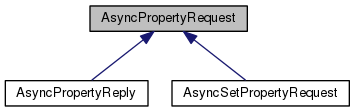
\includegraphics[width=338pt]{classAsyncPropertyRequest__inherit__graph}
\end{center}
\end{figure}
\subsection*{Public Member Functions}
\begin{DoxyCompactItemize}
\item 
\hypertarget{classAsyncPropertyRequest_ad46cfdd3411c11beaa00b70d1c6419d9}{{\bfseries Async\+Property\+Request} (const \hyperlink{classAsyncPropertyRequest}{Async\+Property\+Request} \&request)}\label{classAsyncPropertyRequest_ad46cfdd3411c11beaa00b70d1c6419d9}

\item 
\hypertarget{classAsyncPropertyRequest_ad1de0c87f190106cf70a996e5cba1088}{\hyperlink{classAsyncPropertyRequest}{Async\+Property\+Request} \& {\bfseries operator=} (const \hyperlink{classAsyncPropertyRequest}{Async\+Property\+Request} \&other)}\label{classAsyncPropertyRequest_ad1de0c87f190106cf70a996e5cba1088}

\end{DoxyCompactItemize}
\subsection*{Public Attributes}
\begin{DoxyCompactItemize}
\item 
\hypertarget{classAsyncPropertyRequest_a221de270e3fb828ddbe821aa484a553f}{Vehicle\+Property\+::\+Property \hyperlink{classAsyncPropertyRequest_a221de270e3fb828ddbe821aa484a553f}{property}}\label{classAsyncPropertyRequest_a221de270e3fb828ddbe821aa484a553f}

\begin{DoxyCompactList}\small\item\em property property to request. \end{DoxyCompactList}\item 
\hypertarget{classAsyncPropertyRequest_a2250e8d29929dd879de141049ec78302}{std\+::string \hyperlink{classAsyncPropertyRequest_a2250e8d29929dd879de141049ec78302}{source\+Uuid\+Filter}}\label{classAsyncPropertyRequest_a2250e8d29929dd879de141049ec78302}

\begin{DoxyCompactList}\small\item\em source\+Uuid\+Filter the requesting sink should use this to filter on a specific source or leave blank to use any source \end{DoxyCompactList}\item 
\hypertarget{classAsyncPropertyRequest_a1a19d4677523d8934abe1ddfec5ba1b7}{Zone\+::\+Type \hyperlink{classAsyncPropertyRequest_a1a19d4677523d8934abe1ddfec5ba1b7}{zone\+Filter}}\label{classAsyncPropertyRequest_a1a19d4677523d8934abe1ddfec5ba1b7}

\begin{DoxyCompactList}\small\item\em zone\+Filter the requesting sink should use this if he wants to filter on a specific zone \end{DoxyCompactList}\item 
\hypertarget{classAsyncPropertyRequest_a12e1115b879ffc69a4d9bfd34df3e4be}{Get\+Property\+Completed\+Signal \hyperlink{classAsyncPropertyRequest_a12e1115b879ffc69a4d9bfd34df3e4be}{completed}}\label{classAsyncPropertyRequest_a12e1115b879ffc69a4d9bfd34df3e4be}

\begin{DoxyCompactList}\small\item\em completed the callback when the request has been completed. \end{DoxyCompactList}\item 
uint \hyperlink{classAsyncPropertyRequest_a449da60204ce7c13462be179f869105c}{timeout}
\begin{DoxyCompactList}\small\item\em use to specify a timeout in ms for the request. When a timeout occurs, the 'completed' callback will be called with an error. \end{DoxyCompactList}\item 
\hypertarget{classAsyncPropertyRequest_abaa035426c3ac48fe53de273b1a60eba}{std\+::string \hyperlink{classAsyncPropertyRequest_abaa035426c3ac48fe53de273b1a60eba}{pid}}\label{classAsyncPropertyRequest_abaa035426c3ac48fe53de273b1a60eba}

\begin{DoxyCompactList}\small\item\em pid requesting process id \end{DoxyCompactList}\end{DoxyCompactItemize}


\subsection{Detailed Description}
The \hyperlink{classAsyncPropertyRequest}{Async\+Property\+Request} class is used by sinks to request property values. 

\begin{DoxySeeAlso}{See also}
\hyperlink{classAbstractRoutingEngine_ad1cbda415f674be4a3ce49be05aa8ee8}{Abstract\+Routing\+Engine\+::get\+Property\+Async} 

\hyperlink{classAsyncPropertyReply}{Async\+Property\+Reply} 
\end{DoxySeeAlso}


\subsection{Member Data Documentation}
\hypertarget{classAsyncPropertyRequest_a449da60204ce7c13462be179f869105c}{\index{Async\+Property\+Request@{Async\+Property\+Request}!timeout@{timeout}}
\index{timeout@{timeout}!Async\+Property\+Request@{Async\+Property\+Request}}
\subsubsection[{timeout}]{\setlength{\rightskip}{0pt plus 5cm}uint Async\+Property\+Request\+::timeout}}\label{classAsyncPropertyRequest_a449da60204ce7c13462be179f869105c}


use to specify a timeout in ms for the request. When a timeout occurs, the 'completed' callback will be called with an error. 

\begin{DoxySeeAlso}{See also}
\hyperlink{classAsyncPropertyReply}{Async\+Property\+Reply} default value is\+: 10000 ms 
\end{DoxySeeAlso}


The documentation for this class was generated from the following file\+:\begin{DoxyCompactItemize}
\item 
/home/kev/src/automotive-\/message-\/broker/lib/abstractroutingengine.\+h\end{DoxyCompactItemize}

\hypertarget{structamb_1_1AsyncQueueSource}{\section{amb\+:\+:Async\+Queue\+Source$<$ T, Pred $>$ Struct Template Reference}
\label{structamb_1_1AsyncQueueSource}\index{amb\+::\+Async\+Queue\+Source$<$ T, Pred $>$@{amb\+::\+Async\+Queue\+Source$<$ T, Pred $>$}}
}
\subsection*{Public Attributes}
\begin{DoxyCompactItemize}
\item 
\hypertarget{structamb_1_1AsyncQueueSource_a24c5fe3fdd11cfa92ec95ad440966572}{G\+Source {\bfseries source}}\label{structamb_1_1AsyncQueueSource_a24c5fe3fdd11cfa92ec95ad440966572}

\item 
\hypertarget{structamb_1_1AsyncQueueSource_ac43bbfc0e2112f433ef4cb908fb5e8fc}{\hyperlink{classamb_1_1Queue}{Queue}$<$ T, Pred $>$ $\ast$ {\bfseries queue}}\label{structamb_1_1AsyncQueueSource_ac43bbfc0e2112f433ef4cb908fb5e8fc}

\item 
\hypertarget{structamb_1_1AsyncQueueSource_a1659121d3c53ed3aaab7a7fd6226f2ca}{int {\bfseries min\+Queue\+Size}}\label{structamb_1_1AsyncQueueSource_a1659121d3c53ed3aaab7a7fd6226f2ca}

\end{DoxyCompactItemize}


The documentation for this struct was generated from the following file\+:\begin{DoxyCompactItemize}
\item 
/home/kev/src/automotive-\/message-\/broker/lib/asyncqueue.\+hpp\end{DoxyCompactItemize}

\hypertarget{classamb_1_1AsyncQueueWatcher}{\section{amb\-:\-:Async\-Queue\-Watcher$<$ T, Pred $>$ Class Template Reference}
\label{classamb_1_1AsyncQueueWatcher}\index{amb\-::\-Async\-Queue\-Watcher$<$ T, Pred $>$@{amb\-::\-Async\-Queue\-Watcher$<$ T, Pred $>$}}
}
\subsection*{Public Types}
\begin{DoxyCompactItemize}
\item 
\hypertarget{classamb_1_1AsyncQueueWatcher_a6516f6046d2da8f05b0b8e995c9d266d}{typedef function$<$ void(\hyperlink{classamb_1_1Queue}{Queue}\\*
$<$ T, Pred $>$ $\ast$)$>$ {\bfseries Async\-Queue\-Watcher\-Callback}}\label{classamb_1_1AsyncQueueWatcher_a6516f6046d2da8f05b0b8e995c9d266d}

\end{DoxyCompactItemize}
\subsection*{Public Member Functions}
\begin{DoxyCompactItemize}
\item 
\hypertarget{classamb_1_1AsyncQueueWatcher_a81e2e8e45fe104c1368a7ef250ce7469}{{\bfseries Async\-Queue\-Watcher} (\hyperlink{classamb_1_1Queue}{Queue}$<$ T, Pred $>$ $\ast$queue, Async\-Queue\-Watcher\-Callback cb, int queue\-Size=0, \hyperlink{classAbstractPropertyType_a1e513f66eb2dd2bd2cddbec16422af63}{Abstract\-Property\-Type\-::\-Priority} priority=\hyperlink{classAbstractPropertyType_a1e513f66eb2dd2bd2cddbec16422af63a3412bc77a6a781fb4a832059f1fe5d9a}{Abstract\-Property\-Type\-::\-Normal})}\label{classamb_1_1AsyncQueueWatcher_a81e2e8e45fe104c1368a7ef250ce7469}

\end{DoxyCompactItemize}
\subsection*{Public Attributes}
\begin{DoxyCompactItemize}
\item 
\hypertarget{classamb_1_1AsyncQueueWatcher_a0112d0e35911204b96256e913a065bdb}{Async\-Queue\-Watcher\-Callback {\bfseries callback}}\label{classamb_1_1AsyncQueueWatcher_a0112d0e35911204b96256e913a065bdb}

\end{DoxyCompactItemize}
\subsection*{Protected Attributes}
\begin{DoxyCompactItemize}
\item 
\hypertarget{classamb_1_1AsyncQueueWatcher_a2dd2243a734ce4cd960f689e5cd9988c}{int {\bfseries m\-Max\-Queue\-Size}}\label{classamb_1_1AsyncQueueWatcher_a2dd2243a734ce4cd960f689e5cd9988c}

\end{DoxyCompactItemize}


The documentation for this class was generated from the following file\-:\begin{DoxyCompactItemize}
\item 
/home/tripzero/src/automotive-\/message-\/broker/lib/asyncqueue.\-hpp\end{DoxyCompactItemize}

\hypertarget{classAsyncRangePropertyReply}{\section{Async\+Range\+Property\+Reply Class Reference}
\label{classAsyncRangePropertyReply}\index{Async\+Range\+Property\+Reply@{Async\+Range\+Property\+Reply}}
}


The \hyperlink{classAsyncRangePropertyReply}{Async\+Range\+Property\+Reply} class is used by a source to reply to an \hyperlink{classAsyncRangePropertyRequest}{Async\+Range\+Property\+Request}. The source should set success to 'true' and populate the 'values' member if the request was successful. If the request is not successful, 'success' should be set to 'false' and the 'error' member should be set.  




{\ttfamily \#include $<$abstractroutingengine.\+h$>$}



Inheritance diagram for Async\+Range\+Property\+Reply\+:\nopagebreak
\begin{figure}[H]
\begin{center}
\leavevmode
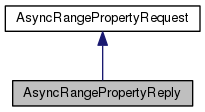
\includegraphics[width=226pt]{classAsyncRangePropertyReply__inherit__graph}
\end{center}
\end{figure}


Collaboration diagram for Async\+Range\+Property\+Reply\+:\nopagebreak
\begin{figure}[H]
\begin{center}
\leavevmode
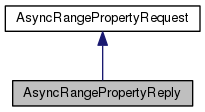
\includegraphics[width=226pt]{classAsyncRangePropertyReply__coll__graph}
\end{center}
\end{figure}
\subsection*{Public Member Functions}
\begin{DoxyCompactItemize}
\item 
\hypertarget{classAsyncRangePropertyReply_ac253016c5ff4dc8e0ac11f8e98a16025}{{\bfseries Async\+Range\+Property\+Reply} (\hyperlink{classAsyncRangePropertyRequest}{Async\+Range\+Property\+Request} request)}\label{classAsyncRangePropertyReply_ac253016c5ff4dc8e0ac11f8e98a16025}

\end{DoxyCompactItemize}
\subsection*{Public Attributes}
\begin{DoxyCompactItemize}
\item 
\hypertarget{classAsyncRangePropertyReply_a43762c9a2d88ec91e3218f7eca297e56}{\hyperlink{classAsyncPropertyReply_ad91affaa25fcc3b73947a6cf4591e5d1}{Async\+Property\+Reply\+::\+Error} \hyperlink{classAsyncRangePropertyReply_a43762c9a2d88ec91e3218f7eca297e56}{error}}\label{classAsyncRangePropertyReply_a43762c9a2d88ec91e3218f7eca297e56}

\begin{DoxyCompactList}\small\item\em error this is set if there was an error in the request. \char`\"{}success\char`\"{} will also be set to false. \end{DoxyCompactList}\item 
\hypertarget{classAsyncRangePropertyReply_a4ce96fd40ce8ec3fddab46652026734b}{std\+::list$<$ \hyperlink{classAbstractPropertyType}{Abstract\+Property\+Type} $\ast$ $>$ \hyperlink{classAsyncRangePropertyReply_a4ce96fd40ce8ec3fddab46652026734b}{values}}\label{classAsyncRangePropertyReply_a4ce96fd40ce8ec3fddab46652026734b}

\begin{DoxyCompactList}\small\item\em values if the request was successful, this will contain a list of values meeting the criteria of the request. \end{DoxyCompactList}\item 
\hypertarget{classAsyncRangePropertyReply_a4eab37dada60970211e62b0fc3aeac92}{bool \hyperlink{classAsyncRangePropertyReply_a4eab37dada60970211e62b0fc3aeac92}{success}}\label{classAsyncRangePropertyReply_a4eab37dada60970211e62b0fc3aeac92}

\begin{DoxyCompactList}\small\item\em success this will be true if the request was successful. If not, this is false and error is set. \end{DoxyCompactList}\end{DoxyCompactItemize}


\subsection{Detailed Description}
The \hyperlink{classAsyncRangePropertyReply}{Async\+Range\+Property\+Reply} class is used by a source to reply to an \hyperlink{classAsyncRangePropertyRequest}{Async\+Range\+Property\+Request}. The source should set success to 'true' and populate the 'values' member if the request was successful. If the request is not successful, 'success' should be set to 'false' and the 'error' member should be set. 

The documentation for this class was generated from the following file\+:\begin{DoxyCompactItemize}
\item 
/home/kev/src/automotive-\/message-\/broker/lib/abstractroutingengine.\+h\end{DoxyCompactItemize}

\hypertarget{classAsyncRangePropertyRequest}{\section{Async\-Range\-Property\-Request Class Reference}
\label{classAsyncRangePropertyRequest}\index{Async\-Range\-Property\-Request@{Async\-Range\-Property\-Request}}
}


The \hyperlink{classAsyncRangePropertyRequest}{Async\-Range\-Property\-Request} class is used by sinks to request values within a time or sequence range.  




{\ttfamily \#include $<$abstractroutingengine.\-h$>$}

Inheritance diagram for Async\-Range\-Property\-Request\-:\begin{figure}[H]
\begin{center}
\leavevmode
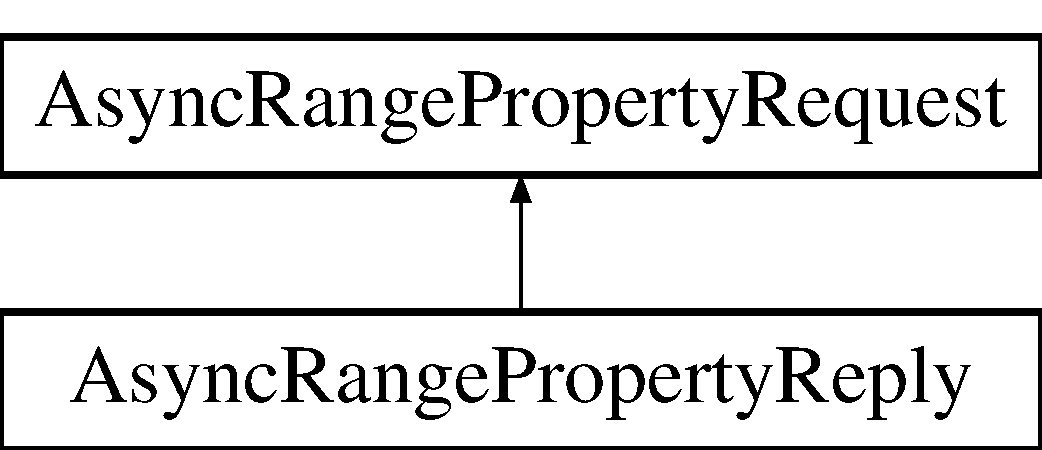
\includegraphics[height=2.000000cm]{classAsyncRangePropertyRequest}
\end{center}
\end{figure}
\subsection*{Public Member Functions}
\begin{DoxyCompactItemize}
\item 
\hypertarget{classAsyncRangePropertyRequest_aefe0f0167ce9bcabcd4450a21c7ea0e5}{{\bfseries Async\-Range\-Property\-Request} (const \hyperlink{classAsyncRangePropertyRequest}{Async\-Range\-Property\-Request} \&request)}\label{classAsyncRangePropertyRequest_aefe0f0167ce9bcabcd4450a21c7ea0e5}

\end{DoxyCompactItemize}
\subsection*{Public Attributes}
\begin{DoxyCompactItemize}
\item 
\hypertarget{classAsyncRangePropertyRequest_afd6f95a06376fef905faf5ab1b580bc9}{Property\-List \hyperlink{classAsyncRangePropertyRequest_afd6f95a06376fef905faf5ab1b580bc9}{properties}}\label{classAsyncRangePropertyRequest_afd6f95a06376fef905faf5ab1b580bc9}

\begin{DoxyCompactList}\small\item\em properties list of properties to request \end{DoxyCompactList}\item 
\hypertarget{classAsyncRangePropertyRequest_a626258d5d401e0598d619b84600689f9}{std\-::string \hyperlink{classAsyncRangePropertyRequest_a626258d5d401e0598d619b84600689f9}{source\-Uuid}}\label{classAsyncRangePropertyRequest_a626258d5d401e0598d619b84600689f9}

\begin{DoxyCompactList}\small\item\em source\-Uuid if the sink wishes to request a specific source, this should be set to the uuid of the source. \end{DoxyCompactList}\item 
\hypertarget{classAsyncRangePropertyRequest_a045f1320e9152de5e97f0b4de5c061da}{Zone\-::\-Type \hyperlink{classAsyncRangePropertyRequest_a045f1320e9152de5e97f0b4de5c061da}{zone}}\label{classAsyncRangePropertyRequest_a045f1320e9152de5e97f0b4de5c061da}

\begin{DoxyCompactList}\small\item\em zone if the sink wishes to request a specific zone, this should be set to the desired zone . \end{DoxyCompactList}\item 
\hypertarget{classAsyncRangePropertyRequest_a81777a8e0304bd6929c05d39c650454d}{Get\-Ranged\-Property\-Completed\-Signal \hyperlink{classAsyncRangePropertyRequest_a81777a8e0304bd6929c05d39c650454d}{completed}}\label{classAsyncRangePropertyRequest_a81777a8e0304bd6929c05d39c650454d}

\begin{DoxyCompactList}\small\item\em completed callback that is called when the ranged request is complete. The reply from this request is passed into the completed call. The completed callback must free the reply before it returns or there will be a leak. \end{DoxyCompactList}\item 
\hypertarget{classAsyncRangePropertyRequest_a2dc2927f6c771707f15a767358a58e69}{double \hyperlink{classAsyncRangePropertyRequest_a2dc2927f6c771707f15a767358a58e69}{time\-Begin}}\label{classAsyncRangePropertyRequest_a2dc2927f6c771707f15a767358a58e69}

\begin{DoxyCompactList}\small\item\em time\-Begin set this to request values for the specified property beggining at this time. Time is seconds\textbackslash{} since the unix epoc. Set this to '0' if you do not want values within a time range. \end{DoxyCompactList}\item 
\hypertarget{classAsyncRangePropertyRequest_acd2a28137c227b0fb6a51576d84f5f30}{double \hyperlink{classAsyncRangePropertyRequest_acd2a28137c227b0fb6a51576d84f5f30}{time\-End}}\label{classAsyncRangePropertyRequest_acd2a28137c227b0fb6a51576d84f5f30}

\begin{DoxyCompactList}\small\item\em time\-End set this to request values for the specified property beggining at this time. Time is seconds\textbackslash{} since the unix epoc. Set this to '0' if you do not want values within a time range. \end{DoxyCompactList}\item 
\hypertarget{classAsyncRangePropertyRequest_a024dab8e12c45ea8988b7f3e4b3c85c0}{int32\-\_\-t \hyperlink{classAsyncRangePropertyRequest_a024dab8e12c45ea8988b7f3e4b3c85c0}{sequence\-Begin}}\label{classAsyncRangePropertyRequest_a024dab8e12c45ea8988b7f3e4b3c85c0}

\begin{DoxyCompactList}\small\item\em sequence\-Begin set this to request values with a sequence $>$= to the sequence\-Begin value. Set to -\/1 if you don't want values within a sequence ranges. \end{DoxyCompactList}\item 
\hypertarget{classAsyncRangePropertyRequest_a352afdecef1d1e6fc1f82384d0c9edfe}{int32\-\_\-t \hyperlink{classAsyncRangePropertyRequest_a352afdecef1d1e6fc1f82384d0c9edfe}{sequence\-End}}\label{classAsyncRangePropertyRequest_a352afdecef1d1e6fc1f82384d0c9edfe}

\begin{DoxyCompactList}\small\item\em sequence\-End set this to request values with a sequence $<$= to the sequence\-End value. Set to -\/1 if you don't want values within a sequence ranges. \end{DoxyCompactList}\item 
\hypertarget{classAsyncRangePropertyRequest_ab93b9cc82ead929a6e1f72be699fbb6c}{std\-::string \hyperlink{classAsyncRangePropertyRequest_ab93b9cc82ead929a6e1f72be699fbb6c}{pid}}\label{classAsyncRangePropertyRequest_ab93b9cc82ead929a6e1f72be699fbb6c}

\begin{DoxyCompactList}\small\item\em pid requesting process id \end{DoxyCompactList}\end{DoxyCompactItemize}


\subsection{Detailed Description}
The \hyperlink{classAsyncRangePropertyRequest}{Async\-Range\-Property\-Request} class is used by sinks to request values within a time or sequence range. 

\begin{DoxySeeAlso}{See Also}
Abstract\-Routing\-Engine\-::get\-Range\-Property\-Async 
\end{DoxySeeAlso}


The documentation for this class was generated from the following file\-:\begin{DoxyCompactItemize}
\item 
/home/kev/src/automotive-\/message-\/broker/lib/abstractroutingengine.\-h\end{DoxyCompactItemize}

\hypertarget{classAsyncSetPropertyRequest}{\section{Async\+Set\+Property\+Request Class Reference}
\label{classAsyncSetPropertyRequest}\index{Async\+Set\+Property\+Request@{Async\+Set\+Property\+Request}}
}


The \hyperlink{classAsyncSetPropertyRequest}{Async\+Set\+Property\+Request} class is used by sinks to set a property to the 'value'. The source will reply with a \hyperlink{classAsyncPropertyReply}{Async\+Property\+Reply} containing the new value or an error.  




{\ttfamily \#include $<$abstractroutingengine.\+h$>$}



Inheritance diagram for Async\+Set\+Property\+Request\+:\nopagebreak
\begin{figure}[H]
\begin{center}
\leavevmode
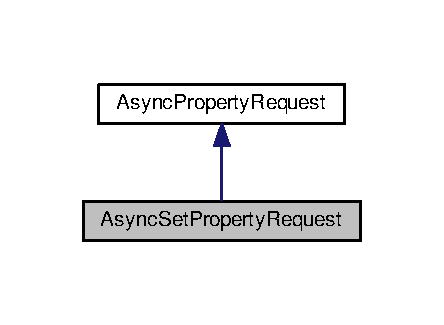
\includegraphics[width=213pt]{classAsyncSetPropertyRequest__inherit__graph}
\end{center}
\end{figure}


Collaboration diagram for Async\+Set\+Property\+Request\+:\nopagebreak
\begin{figure}[H]
\begin{center}
\leavevmode
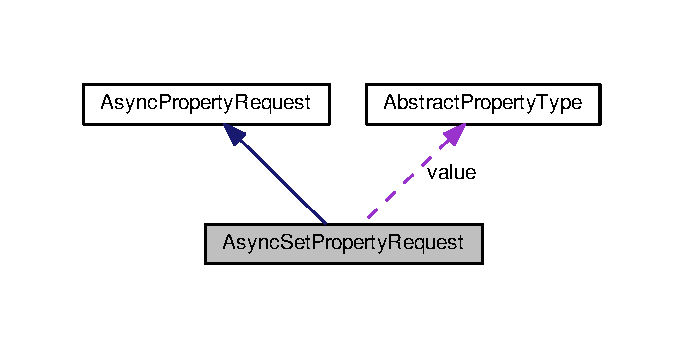
\includegraphics[width=328pt]{classAsyncSetPropertyRequest__coll__graph}
\end{center}
\end{figure}
\subsection*{Public Member Functions}
\begin{DoxyCompactItemize}
\item 
\hypertarget{classAsyncSetPropertyRequest_aa2fa61c815aa1950511eb88cc29f655a}{{\bfseries Async\+Set\+Property\+Request} (const \hyperlink{classAsyncPropertyRequest}{Async\+Property\+Request} \&request)}\label{classAsyncSetPropertyRequest_aa2fa61c815aa1950511eb88cc29f655a}

\end{DoxyCompactItemize}
\subsection*{Public Attributes}
\begin{DoxyCompactItemize}
\item 
\hypertarget{classAsyncSetPropertyRequest_a5c1c8d5b4a6765ce2acab9a3aca9c9a6}{\hyperlink{classAbstractPropertyType}{Abstract\+Property\+Type} $\ast$ \hyperlink{classAsyncSetPropertyRequest_a5c1c8d5b4a6765ce2acab9a3aca9c9a6}{value}}\label{classAsyncSetPropertyRequest_a5c1c8d5b4a6765ce2acab9a3aca9c9a6}

\begin{DoxyCompactList}\small\item\em value the new value to set the property to. \end{DoxyCompactList}\end{DoxyCompactItemize}


\subsection{Detailed Description}
The \hyperlink{classAsyncSetPropertyRequest}{Async\+Set\+Property\+Request} class is used by sinks to set a property to the 'value'. The source will reply with a \hyperlink{classAsyncPropertyReply}{Async\+Property\+Reply} containing the new value or an error. 

\begin{DoxySeeAlso}{See also}
Abstract\+Routing\+Engine\+::set\+Property 

\hyperlink{classAsyncPropertyReply}{Async\+Property\+Reply} 
\end{DoxySeeAlso}


The documentation for this class was generated from the following file\+:\begin{DoxyCompactItemize}
\item 
/home/kev/src/automotive-\/message-\/broker/lib/abstractroutingengine.\+h\end{DoxyCompactItemize}

\hypertarget{classBasicPropertyType}{\section{Basic\-Property\-Type$<$ T $>$ Class Template Reference}
\label{classBasicPropertyType}\index{Basic\-Property\-Type$<$ T $>$@{Basic\-Property\-Type$<$ T $>$}}
}
Inheritance diagram for Basic\-Property\-Type$<$ T $>$\-:\begin{figure}[H]
\begin{center}
\leavevmode
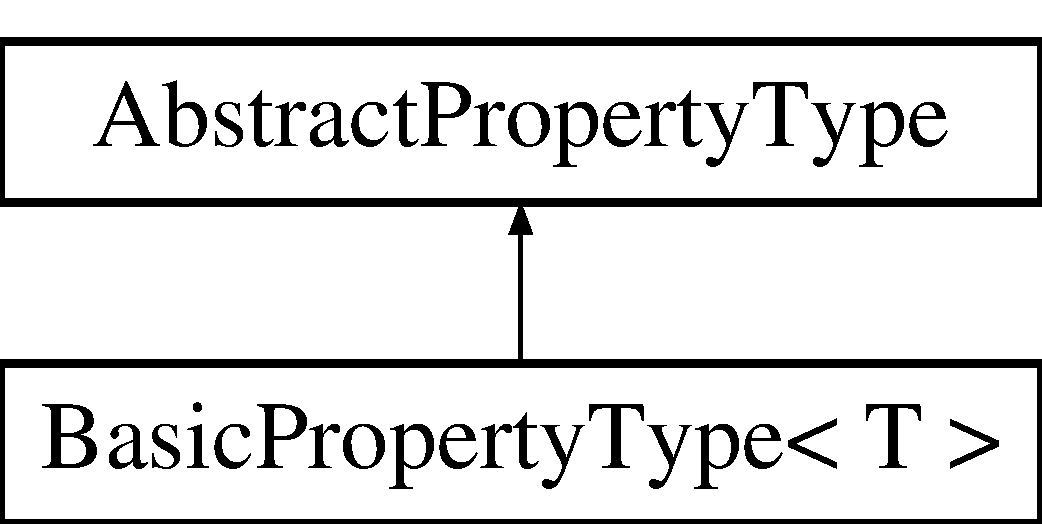
\includegraphics[height=2.000000cm]{classBasicPropertyType}
\end{center}
\end{figure}
\subsection*{Public Member Functions}
\begin{DoxyCompactItemize}
\item 
\hypertarget{classBasicPropertyType_a9d967556ec7106be014ef360e8ad729c}{{\bfseries Basic\-Property\-Type} (\hyperlink{classBasicPropertyType}{Basic\-Property\-Type} const \&other)}\label{classBasicPropertyType_a9d967556ec7106be014ef360e8ad729c}

\item 
\hypertarget{classBasicPropertyType_adf19305750a4f3aaf605ae2b18353e32}{\hyperlink{classBasicPropertyType}{Basic\-Property\-Type} \& {\bfseries operator=} (\hyperlink{classBasicPropertyType}{Basic\-Property\-Type} const \&other)}\label{classBasicPropertyType_adf19305750a4f3aaf605ae2b18353e32}

\item 
\hypertarget{classBasicPropertyType_ae2a1d3c9885b05c9d022d1a01e28888e}{bool {\bfseries operator$<$} (const \hyperlink{classBasicPropertyType}{Basic\-Property\-Type}$<$ T $>$ \&other) const }\label{classBasicPropertyType_ae2a1d3c9885b05c9d022d1a01e28888e}

\item 
\hypertarget{classBasicPropertyType_a6cb6f98a17ae2ae19c94643de930a73c}{bool {\bfseries operator$>$} (const \hyperlink{classBasicPropertyType}{Basic\-Property\-Type}$<$ T $>$ \&other) const }\label{classBasicPropertyType_a6cb6f98a17ae2ae19c94643de930a73c}

\item 
\hypertarget{classBasicPropertyType_a0fcc2038187aad4b1ee6223daaff65d6}{{\bfseries Basic\-Property\-Type} (T val)}\label{classBasicPropertyType_a0fcc2038187aad4b1ee6223daaff65d6}

\item 
\hypertarget{classBasicPropertyType_a5336941eaf15eefbfc9f84554619b72d}{{\bfseries Basic\-Property\-Type} (std\-::string property\-Name, T val)}\label{classBasicPropertyType_a5336941eaf15eefbfc9f84554619b72d}

\item 
\hypertarget{classBasicPropertyType_a1bb538ecec45a113bbfc1fa23eabfde1}{{\bfseries Basic\-Property\-Type} (std\-::string property\-Name, std\-::string val)}\label{classBasicPropertyType_a1bb538ecec45a113bbfc1fa23eabfde1}

\item 
\hypertarget{classBasicPropertyType_a4f8b38f1e145d5ee7387a58faaef8e60}{{\bfseries Basic\-Property\-Type} (std\-::string property\-Name)}\label{classBasicPropertyType_a4f8b38f1e145d5ee7387a58faaef8e60}

\item 
\hypertarget{classBasicPropertyType_a244d19253bfc42dfadd84570b8c8e404}{\hyperlink{classAbstractPropertyType}{Abstract\-Property\-Type} $\ast$ {\bfseries copy} ()}\label{classBasicPropertyType_a244d19253bfc42dfadd84570b8c8e404}

\item 
\hypertarget{classBasicPropertyType_a3c73a6a2c2c020ec327849f318ae9f2a}{void {\bfseries from\-String} (std\-::string val)}\label{classBasicPropertyType_a3c73a6a2c2c020ec327849f318ae9f2a}

\item 
\hypertarget{classBasicPropertyType_a672e2824bcc38da6e60090022fd8d114}{std\-::string {\bfseries to\-String} () const }\label{classBasicPropertyType_a672e2824bcc38da6e60090022fd8d114}

\item 
\hypertarget{classBasicPropertyType_a893a2d1f8fec7141159d850caa78bc06}{G\-Variant $\ast$ {\bfseries to\-Variant} ()}\label{classBasicPropertyType_a893a2d1f8fec7141159d850caa78bc06}

\item 
\hypertarget{classBasicPropertyType_a0e1213ee2df11ecd556b250fe3bad21b}{void {\bfseries from\-Variant} (G\-Variant $\ast$v)}\label{classBasicPropertyType_a0e1213ee2df11ecd556b250fe3bad21b}

\end{DoxyCompactItemize}
\subsection*{Additional Inherited Members}


The documentation for this class was generated from the following file\-:\begin{DoxyCompactItemize}
\item 
/home/kev/src/automotive-\/message-\/broker/lib/abstractpropertytype.\-h\end{DoxyCompactItemize}

\hypertarget{classDebugOut}{\section{Debug\+Out Class Reference}
\label{classDebugOut}\index{Debug\+Out@{Debug\+Out}}
}


The \hyperlink{classDebugOut}{Debug\+Out} class represents a class used for outputing debug information The specified debug level will only be outputed if the debug level is =$>$ the debug threshhold Here's a simple example\+:  




{\ttfamily \#include $<$debugout.\+h$>$}

\subsection*{Public Member Functions}
\begin{DoxyCompactItemize}
\item 
\hypertarget{classDebugOut_a833f5ea5ab0d98d3fdf4a1ed8efed770}{{\bfseries Debug\+Out} (int debug\+Level=4)}\label{classDebugOut_a833f5ea5ab0d98d3fdf4a1ed8efed770}

\item 
\hypertarget{classDebugOut_aa35622f0f1b15060ad0f281de6e799b3}{\hyperlink{classDebugOut}{Debug\+Out} const \& {\bfseries operator$<$$<$} (const string \&message) const }\label{classDebugOut_aa35622f0f1b15060ad0f281de6e799b3}

\item 
\hypertarget{classDebugOut_a0b83635c229210d6000b9663575bbe99}{\hyperlink{classDebugOut}{Debug\+Out} const \& {\bfseries operator$<$$<$} (ostream \&($\ast$manip)(std\+::ostream \&)) const }\label{classDebugOut_a0b83635c229210d6000b9663575bbe99}

\item 
\hypertarget{classDebugOut_a9ab6e54c6f70bcbf18faf329952b5998}{\hyperlink{classDebugOut}{Debug\+Out} const \& {\bfseries operator$<$$<$} (double val) const }\label{classDebugOut_a9ab6e54c6f70bcbf18faf329952b5998}

\end{DoxyCompactItemize}
\subsection*{Static Public Member Functions}
\begin{DoxyCompactItemize}
\item 
\hypertarget{classDebugOut_a5eb2fb8c9db45f812b5dadb2fd63dcee}{static void {\bfseries set\+Debug\+Threshhold} (int th)}\label{classDebugOut_a5eb2fb8c9db45f812b5dadb2fd63dcee}

\item 
\hypertarget{classDebugOut_a89fc39319cc80007a0188b831fae32c1}{static void {\bfseries set\+Output} (ostream \&o)}\label{classDebugOut_a89fc39319cc80007a0188b831fae32c1}

\item 
\hypertarget{classDebugOut_a0651b00c0d62d93a9c57209874b2650c}{static void {\bfseries set\+Throw\+Warn} (bool v)}\label{classDebugOut_a0651b00c0d62d93a9c57209874b2650c}

\item 
\hypertarget{classDebugOut_a59402f0300c1b41f7290c8274cd08c58}{static void {\bfseries set\+Throw\+Err} (bool v)}\label{classDebugOut_a59402f0300c1b41f7290c8274cd08c58}

\item 
\hypertarget{classDebugOut_af4903a2f68a012000cc91562d0183e2a}{static const int {\bfseries get\+Debug\+Threshhold} ()}\label{classDebugOut_af4903a2f68a012000cc91562d0183e2a}

\end{DoxyCompactItemize}
\subsection*{Static Public Attributes}
\begin{DoxyCompactItemize}
\item 
\hypertarget{classDebugOut_a40314aef0df2ed8a705d9372d49b0535}{static const int \hyperlink{classDebugOut_a40314aef0df2ed8a705d9372d49b0535}{Error} = 1 $<$$<$ 16}\label{classDebugOut_a40314aef0df2ed8a705d9372d49b0535}

\begin{DoxyCompactList}\small\item\em Error use when essential functionality is blocked. \end{DoxyCompactList}\item 
\hypertarget{classDebugOut_a7a06aa04dd6cb8c1e9bcd083d30d91ad}{static const int \hyperlink{classDebugOut_a7a06aa04dd6cb8c1e9bcd083d30d91ad}{Warning} = 1 $<$$<$ 24}\label{classDebugOut_a7a06aa04dd6cb8c1e9bcd083d30d91ad}

\begin{DoxyCompactList}\small\item\em Warning use when non-\/essential functionality is bocked, or when workarounds exist. \end{DoxyCompactList}\end{DoxyCompactItemize}


\subsection{Detailed Description}
The \hyperlink{classDebugOut}{Debug\+Out} class represents a class used for outputing debug information The specified debug level will only be outputed if the debug level is =$>$ the debug threshhold Here's a simple example\+: 


\begin{DoxyCode}
DebugOut::setDebugThreshhold(3);
\hyperlink{classDebugOut}{DebugOut}(\hyperlink{classDebugOut_a7a06aa04dd6cb8c1e9bcd083d30d91ad}{DebugOut::Warning}) << \textcolor{stringliteral}{"This is a warning"} << std::endl;
\hyperlink{classDebugOut}{DebugOut}(3) << \textcolor{stringliteral}{"This will only show if the threshhold is 3 or lower."} << std::endl;

ofstream logfile;
logfile.open(\textcolor{stringliteral}{"amb.log"}, ios::out | ios::trunc);
DebugOut::setOutput(logfile)

\hyperlink{classDebugOut}{DebugOut}::setThrowErr(true);
\hyperlink{classDebugOut}{DebugOut}::setThrowWarn(true);
\hyperlink{classDebugOut}{DebugOut}(\hyperlink{classDebugOut}{DebugOut}::\hyperlink{classDebugOut_a40314aef0df2ed8a705d9372d49b0535}{Error}) << "This will throw an exception." << 
      \hyperlink{namespacestd}{std}::endl;

\hyperlink{classDebugOut}{DebugOut}::setOutput(\hyperlink{namespacestd}{std}::cerr);
\hyperlink{classDebugOut}{DebugOut}() << "This will log to stderr." << \hyperlink{namespacestd}{std}::endl;
\end{DoxyCode}
 

The documentation for this class was generated from the following files\+:\begin{DoxyCompactItemize}
\item 
/home/kev/src/automotive-\/message-\/broker/lib/debugout.\+h\item 
/home/kev/src/automotive-\/message-\/broker/lib/debugout.\+cpp\end{DoxyCompactItemize}

\hypertarget{structamb_1_1traits_3_01GVariant_01_4_1_1delete__functor}{\section{amb\-:\-:traits$<$ G\-Variant $>$\-:\-:delete\-\_\-functor Struct Reference}
\label{structamb_1_1traits_3_01GVariant_01_4_1_1delete__functor}\index{amb\-::traits$<$ G\-Variant $>$\-::delete\-\_\-functor@{amb\-::traits$<$ G\-Variant $>$\-::delete\-\_\-functor}}
}
\subsection*{Public Member Functions}
\begin{DoxyCompactItemize}
\item 
\hypertarget{structamb_1_1traits_3_01GVariant_01_4_1_1delete__functor_aa0393bd9227a3112d0708e3b417de044}{void {\bfseries operator()} (G\-Variant $\ast$p) const }\label{structamb_1_1traits_3_01GVariant_01_4_1_1delete__functor_aa0393bd9227a3112d0708e3b417de044}

\end{DoxyCompactItemize}


The documentation for this struct was generated from the following file\-:\begin{DoxyCompactItemize}
\item 
/home/tripzero/src/automotive-\/message-\/broker/lib/superptr.\-hpp\end{DoxyCompactItemize}

\hypertarget{structamb_1_1traits_3_01GError_01_4_1_1delete__functor}{\section{amb\+:\+:traits$<$ G\+Error $>$\+:\+:delete\+\_\+functor Struct Reference}
\label{structamb_1_1traits_3_01GError_01_4_1_1delete__functor}\index{amb\+::traits$<$ G\+Error $>$\+::delete\+\_\+functor@{amb\+::traits$<$ G\+Error $>$\+::delete\+\_\+functor}}
}
\subsection*{Public Member Functions}
\begin{DoxyCompactItemize}
\item 
\hypertarget{structamb_1_1traits_3_01GError_01_4_1_1delete__functor_ac39ebbfad72facba5348ae7ffcbda46f}{void {\bfseries operator()} (G\+Error $\ast$p) const }\label{structamb_1_1traits_3_01GError_01_4_1_1delete__functor_ac39ebbfad72facba5348ae7ffcbda46f}

\end{DoxyCompactItemize}


The documentation for this struct was generated from the following file\+:\begin{DoxyCompactItemize}
\item 
/home/kev/src/automotive-\/message-\/broker/lib/superptr.\+hpp\end{DoxyCompactItemize}

\hypertarget{structamb_1_1traits_3_01GDBusProxy_01_4_1_1delete__functor}{\section{amb\+:\+:traits$<$ G\+D\+Bus\+Proxy $>$\+:\+:delete\+\_\+functor Struct Reference}
\label{structamb_1_1traits_3_01GDBusProxy_01_4_1_1delete__functor}\index{amb\+::traits$<$ G\+D\+Bus\+Proxy $>$\+::delete\+\_\+functor@{amb\+::traits$<$ G\+D\+Bus\+Proxy $>$\+::delete\+\_\+functor}}
}
\subsection*{Public Member Functions}
\begin{DoxyCompactItemize}
\item 
\hypertarget{structamb_1_1traits_3_01GDBusProxy_01_4_1_1delete__functor_aa6bea2fb8b4ddb29378fa0188652b8da}{void {\bfseries operator()} (G\+D\+Bus\+Proxy $\ast$p) const }\label{structamb_1_1traits_3_01GDBusProxy_01_4_1_1delete__functor_aa6bea2fb8b4ddb29378fa0188652b8da}

\end{DoxyCompactItemize}


The documentation for this struct was generated from the following file\+:\begin{DoxyCompactItemize}
\item 
/home/kev/src/automotive-\/message-\/broker/lib/superptr.\+hpp\end{DoxyCompactItemize}

\hypertarget{structamb_1_1traits_3_01gchar_01_4_1_1delete__functor}{\section{amb\-:\-:traits$<$ gchar $>$\-:\-:delete\-\_\-functor Struct Reference}
\label{structamb_1_1traits_3_01gchar_01_4_1_1delete__functor}\index{amb\-::traits$<$ gchar $>$\-::delete\-\_\-functor@{amb\-::traits$<$ gchar $>$\-::delete\-\_\-functor}}
}
\subsection*{Public Member Functions}
\begin{DoxyCompactItemize}
\item 
\hypertarget{structamb_1_1traits_3_01gchar_01_4_1_1delete__functor_a19eabedff810e940a5104aca5785003a}{void {\bfseries operator()} (gchar $\ast$p) const }\label{structamb_1_1traits_3_01gchar_01_4_1_1delete__functor_a19eabedff810e940a5104aca5785003a}

\end{DoxyCompactItemize}


The documentation for this struct was generated from the following file\-:\begin{DoxyCompactItemize}
\item 
/home/tripzero/src/automotive-\/message-\/broker/lib/superptr.\-hpp\end{DoxyCompactItemize}

\hypertarget{structamb_1_1traits_3_01GVariantIter_01_4_1_1delete__functor}{\section{amb\-:\-:traits$<$ G\-Variant\-Iter $>$\-:\-:delete\-\_\-functor Struct Reference}
\label{structamb_1_1traits_3_01GVariantIter_01_4_1_1delete__functor}\index{amb\-::traits$<$ G\-Variant\-Iter $>$\-::delete\-\_\-functor@{amb\-::traits$<$ G\-Variant\-Iter $>$\-::delete\-\_\-functor}}
}
\subsection*{Public Member Functions}
\begin{DoxyCompactItemize}
\item 
\hypertarget{structamb_1_1traits_3_01GVariantIter_01_4_1_1delete__functor_a28037ddb5e64f1e716abbaa840db1ad5}{void {\bfseries operator()} (G\-Variant\-Iter $\ast$p) const }\label{structamb_1_1traits_3_01GVariantIter_01_4_1_1delete__functor_a28037ddb5e64f1e716abbaa840db1ad5}

\end{DoxyCompactItemize}


The documentation for this struct was generated from the following file\-:\begin{DoxyCompactItemize}
\item 
/home/tripzero/src/automotive-\/message-\/broker/lib/superptr.\-hpp\end{DoxyCompactItemize}

\hypertarget{classGVS}{\section{G\-V\-S$<$ T $>$ Class Template Reference}
\label{classGVS}\index{G\-V\-S$<$ T $>$@{G\-V\-S$<$ T $>$}}
}


The documentation for this class was generated from the following file\-:\begin{DoxyCompactItemize}
\item 
/home/tripzero/src/automotive-\/message-\/broker/lib/abstractpropertytype.\-h\end{DoxyCompactItemize}

\hypertarget{classGVS_3_01bool_01_4}{\section{G\-V\-S$<$ bool $>$ Class Template Reference}
\label{classGVS_3_01bool_01_4}\index{G\-V\-S$<$ bool $>$@{G\-V\-S$<$ bool $>$}}
}
\subsection*{Static Public Member Functions}
\begin{DoxyCompactItemize}
\item 
\hypertarget{classGVS_3_01bool_01_4_a81cb01e07ccf7830cce75abcc4a2cca8}{static const char $\ast$ {\bfseries signature} ()}\label{classGVS_3_01bool_01_4_a81cb01e07ccf7830cce75abcc4a2cca8}

\item 
\hypertarget{classGVS_3_01bool_01_4_affd787db6c549ec8bee51862fc51f211}{static bool {\bfseries value} (G\-Variant $\ast$v)}\label{classGVS_3_01bool_01_4_affd787db6c549ec8bee51862fc51f211}

\item 
\hypertarget{classGVS_3_01bool_01_4_a3f5e4da1a15517ae3e700c3a1b70fea7}{static std\-::string {\bfseries stringize} (std\-::string v)}\label{classGVS_3_01bool_01_4_a3f5e4da1a15517ae3e700c3a1b70fea7}

\end{DoxyCompactItemize}


The documentation for this class was generated from the following file\-:\begin{DoxyCompactItemize}
\item 
/home/kev/src/automotive-\/message-\/broker/lib/abstractpropertytype.\-h\end{DoxyCompactItemize}

\hypertarget{classGVS_3_01char_01_4}{\section{G\-V\-S$<$ char $>$ Class Template Reference}
\label{classGVS_3_01char_01_4}\index{G\-V\-S$<$ char $>$@{G\-V\-S$<$ char $>$}}
}
\subsection*{Static Public Member Functions}
\begin{DoxyCompactItemize}
\item 
\hypertarget{classGVS_3_01char_01_4_a99899c615057156f961eee40c3ffa054}{static const char $\ast$ {\bfseries signature} ()}\label{classGVS_3_01char_01_4_a99899c615057156f961eee40c3ffa054}

\item 
\hypertarget{classGVS_3_01char_01_4_a1ea37cc4e2f186ed71296a856bde3ea0}{static char {\bfseries value} (G\-Variant $\ast$v)}\label{classGVS_3_01char_01_4_a1ea37cc4e2f186ed71296a856bde3ea0}

\item 
\hypertarget{classGVS_3_01char_01_4_ab3eb5abbfb3a71184aa7741a5bd25dd8}{static std\-::string {\bfseries stringize} (std\-::string v)}\label{classGVS_3_01char_01_4_ab3eb5abbfb3a71184aa7741a5bd25dd8}

\end{DoxyCompactItemize}


The documentation for this class was generated from the following file\-:\begin{DoxyCompactItemize}
\item 
/home/tripzero/src/automotive-\/message-\/broker/lib/abstractpropertytype.\-h\end{DoxyCompactItemize}

\hypertarget{classGVS_3_01double_01_4}{\section{G\-V\-S$<$ double $>$ Class Template Reference}
\label{classGVS_3_01double_01_4}\index{G\-V\-S$<$ double $>$@{G\-V\-S$<$ double $>$}}
}
\subsection*{Static Public Member Functions}
\begin{DoxyCompactItemize}
\item 
\hypertarget{classGVS_3_01double_01_4_a995d18f59b8a60af292ecb4778378f6a}{static const char $\ast$ {\bfseries signature} ()}\label{classGVS_3_01double_01_4_a995d18f59b8a60af292ecb4778378f6a}

\item 
\hypertarget{classGVS_3_01double_01_4_ab60f061e68f1e60367f62057a0549160}{static double {\bfseries value} (G\-Variant $\ast$v)}\label{classGVS_3_01double_01_4_ab60f061e68f1e60367f62057a0549160}

\item 
\hypertarget{classGVS_3_01double_01_4_aee0d8fdc467f97da7b072b1caa34b694}{static std\-::string {\bfseries stringize} (std\-::string v)}\label{classGVS_3_01double_01_4_aee0d8fdc467f97da7b072b1caa34b694}

\end{DoxyCompactItemize}


The documentation for this class was generated from the following file\-:\begin{DoxyCompactItemize}
\item 
/home/kev/src/automotive-\/message-\/broker/lib/abstractpropertytype.\-h\end{DoxyCompactItemize}

\hypertarget{classGVS_3_01int_01_4}{\section{G\-V\-S$<$ int $>$ Class Template Reference}
\label{classGVS_3_01int_01_4}\index{G\-V\-S$<$ int $>$@{G\-V\-S$<$ int $>$}}
}
\subsection*{Static Public Member Functions}
\begin{DoxyCompactItemize}
\item 
\hypertarget{classGVS_3_01int_01_4_aac00b94bc9b614c9adafdecc671b895e}{static const char $\ast$ {\bfseries signature} ()}\label{classGVS_3_01int_01_4_aac00b94bc9b614c9adafdecc671b895e}

\item 
\hypertarget{classGVS_3_01int_01_4_af57dd531535ceb741c65a90520aba578}{static int {\bfseries value} (G\-Variant $\ast$v)}\label{classGVS_3_01int_01_4_af57dd531535ceb741c65a90520aba578}

\item 
\hypertarget{classGVS_3_01int_01_4_ac284bb5efd7dc2bb3f641c94317a3385}{static std\-::string {\bfseries stringize} (std\-::string v)}\label{classGVS_3_01int_01_4_ac284bb5efd7dc2bb3f641c94317a3385}

\end{DoxyCompactItemize}


The documentation for this class was generated from the following file\-:\begin{DoxyCompactItemize}
\item 
/home/tripzero/src/automotive-\/message-\/broker/lib/abstractpropertytype.\-h\end{DoxyCompactItemize}

\hypertarget{classGVS_3_01int16__t_01_4}{\section{G\-V\-S$<$ int16\-\_\-t $>$ Class Template Reference}
\label{classGVS_3_01int16__t_01_4}\index{G\-V\-S$<$ int16\-\_\-t $>$@{G\-V\-S$<$ int16\-\_\-t $>$}}
}
\subsection*{Static Public Member Functions}
\begin{DoxyCompactItemize}
\item 
\hypertarget{classGVS_3_01int16__t_01_4_a74fd2e54cfeebf2f87376b11a4d7b527}{static const char $\ast$ {\bfseries signature} ()}\label{classGVS_3_01int16__t_01_4_a74fd2e54cfeebf2f87376b11a4d7b527}

\item 
\hypertarget{classGVS_3_01int16__t_01_4_a3b5ee21a1f741c1543bf22738885e460}{static int16\-\_\-t {\bfseries value} (G\-Variant $\ast$v)}\label{classGVS_3_01int16__t_01_4_a3b5ee21a1f741c1543bf22738885e460}

\item 
\hypertarget{classGVS_3_01int16__t_01_4_a8ebde11ede44782a48dc2aecbbb5e3af}{static std\-::string {\bfseries stringize} (std\-::string v)}\label{classGVS_3_01int16__t_01_4_a8ebde11ede44782a48dc2aecbbb5e3af}

\end{DoxyCompactItemize}


The documentation for this class was generated from the following file\-:\begin{DoxyCompactItemize}
\item 
/home/kev/src/automotive-\/message-\/broker/lib/abstractpropertytype.\-h\end{DoxyCompactItemize}

\hypertarget{classGVS_3_01int64__t_01_4}{\section{G\-V\-S$<$ int64\-\_\-t $>$ Class Template Reference}
\label{classGVS_3_01int64__t_01_4}\index{G\-V\-S$<$ int64\-\_\-t $>$@{G\-V\-S$<$ int64\-\_\-t $>$}}
}
\subsection*{Static Public Member Functions}
\begin{DoxyCompactItemize}
\item 
\hypertarget{classGVS_3_01int64__t_01_4_a1dc54b2dda69355ec6c037fe0ee28a68}{static const char $\ast$ {\bfseries signature} ()}\label{classGVS_3_01int64__t_01_4_a1dc54b2dda69355ec6c037fe0ee28a68}

\item 
\hypertarget{classGVS_3_01int64__t_01_4_a08ab99b0ab505b2d29e4e954e91f75e0}{static int64\-\_\-t {\bfseries value} (G\-Variant $\ast$v)}\label{classGVS_3_01int64__t_01_4_a08ab99b0ab505b2d29e4e954e91f75e0}

\item 
\hypertarget{classGVS_3_01int64__t_01_4_a66197d92e5c517a97326ccff42e338bb}{static std\-::string {\bfseries stringize} (std\-::string v)}\label{classGVS_3_01int64__t_01_4_a66197d92e5c517a97326ccff42e338bb}

\end{DoxyCompactItemize}


The documentation for this class was generated from the following file\-:\begin{DoxyCompactItemize}
\item 
/home/kev/src/automotive-\/message-\/broker/lib/abstractpropertytype.\-h\end{DoxyCompactItemize}

\hypertarget{classGVS_3_01uint16__t_01_4}{\section{G\-V\-S$<$ uint16\-\_\-t $>$ Class Template Reference}
\label{classGVS_3_01uint16__t_01_4}\index{G\-V\-S$<$ uint16\-\_\-t $>$@{G\-V\-S$<$ uint16\-\_\-t $>$}}
}
\subsection*{Static Public Member Functions}
\begin{DoxyCompactItemize}
\item 
\hypertarget{classGVS_3_01uint16__t_01_4_a7db0c4a8cd2454cd49ede1fb7a026e49}{static const char $\ast$ {\bfseries signature} ()}\label{classGVS_3_01uint16__t_01_4_a7db0c4a8cd2454cd49ede1fb7a026e49}

\item 
\hypertarget{classGVS_3_01uint16__t_01_4_a629f9b3cba434e8c808d545ca8a8e557}{static uint16\-\_\-t {\bfseries value} (G\-Variant $\ast$v)}\label{classGVS_3_01uint16__t_01_4_a629f9b3cba434e8c808d545ca8a8e557}

\item 
\hypertarget{classGVS_3_01uint16__t_01_4_a4d7e2288bb0be81487945a42e7aa8224}{static std\-::string {\bfseries stringize} (std\-::string v)}\label{classGVS_3_01uint16__t_01_4_a4d7e2288bb0be81487945a42e7aa8224}

\end{DoxyCompactItemize}


The documentation for this class was generated from the following file\-:\begin{DoxyCompactItemize}
\item 
/home/kev/src/automotive-\/message-\/broker/lib/abstractpropertytype.\-h\end{DoxyCompactItemize}

\hypertarget{classGVS_3_01uint32__t_01_4}{\section{G\-V\-S$<$ uint32\-\_\-t $>$ Class Template Reference}
\label{classGVS_3_01uint32__t_01_4}\index{G\-V\-S$<$ uint32\-\_\-t $>$@{G\-V\-S$<$ uint32\-\_\-t $>$}}
}
\subsection*{Static Public Member Functions}
\begin{DoxyCompactItemize}
\item 
\hypertarget{classGVS_3_01uint32__t_01_4_a4ead38a9a6e109e3f8cce37507cdbed5}{static const char $\ast$ {\bfseries signature} ()}\label{classGVS_3_01uint32__t_01_4_a4ead38a9a6e109e3f8cce37507cdbed5}

\item 
\hypertarget{classGVS_3_01uint32__t_01_4_aa71849881fbf20dcca20922bea646007}{static uint32\-\_\-t {\bfseries value} (G\-Variant $\ast$v)}\label{classGVS_3_01uint32__t_01_4_aa71849881fbf20dcca20922bea646007}

\item 
\hypertarget{classGVS_3_01uint32__t_01_4_ac8a872590d86a403b8441b4d0bb03a61}{static std\-::string {\bfseries stringize} (std\-::string v)}\label{classGVS_3_01uint32__t_01_4_ac8a872590d86a403b8441b4d0bb03a61}

\end{DoxyCompactItemize}


The documentation for this class was generated from the following file\-:\begin{DoxyCompactItemize}
\item 
/home/tripzero/src/automotive-\/message-\/broker/lib/abstractpropertytype.\-h\end{DoxyCompactItemize}

\hypertarget{classGVS_3_01uint64__t_01_4}{\section{G\-V\-S$<$ uint64\-\_\-t $>$ Class Template Reference}
\label{classGVS_3_01uint64__t_01_4}\index{G\-V\-S$<$ uint64\-\_\-t $>$@{G\-V\-S$<$ uint64\-\_\-t $>$}}
}
\subsection*{Static Public Member Functions}
\begin{DoxyCompactItemize}
\item 
\hypertarget{classGVS_3_01uint64__t_01_4_af3a581bec16849dd09e5a46a68ee5c9a}{static const char $\ast$ {\bfseries signature} ()}\label{classGVS_3_01uint64__t_01_4_af3a581bec16849dd09e5a46a68ee5c9a}

\item 
\hypertarget{classGVS_3_01uint64__t_01_4_a2d48a0a60faa407a338bf886f8120e44}{static uint64\-\_\-t {\bfseries value} (G\-Variant $\ast$v)}\label{classGVS_3_01uint64__t_01_4_a2d48a0a60faa407a338bf886f8120e44}

\item 
\hypertarget{classGVS_3_01uint64__t_01_4_a85e2ae3bd54dd831724a7cda94bcf5cb}{static std\-::string {\bfseries stringize} (std\-::string v)}\label{classGVS_3_01uint64__t_01_4_a85e2ae3bd54dd831724a7cda94bcf5cb}

\end{DoxyCompactItemize}


The documentation for this class was generated from the following file\-:\begin{DoxyCompactItemize}
\item 
/home/tripzero/src/automotive-\/message-\/broker/lib/abstractpropertytype.\-h\end{DoxyCompactItemize}

\hypertarget{classListPropertyType}{\section{List\-Property\-Type$<$ T $>$ Class Template Reference}
\label{classListPropertyType}\index{List\-Property\-Type$<$ T $>$@{List\-Property\-Type$<$ T $>$}}
}
Inheritance diagram for List\-Property\-Type$<$ T $>$\-:\begin{figure}[H]
\begin{center}
\leavevmode
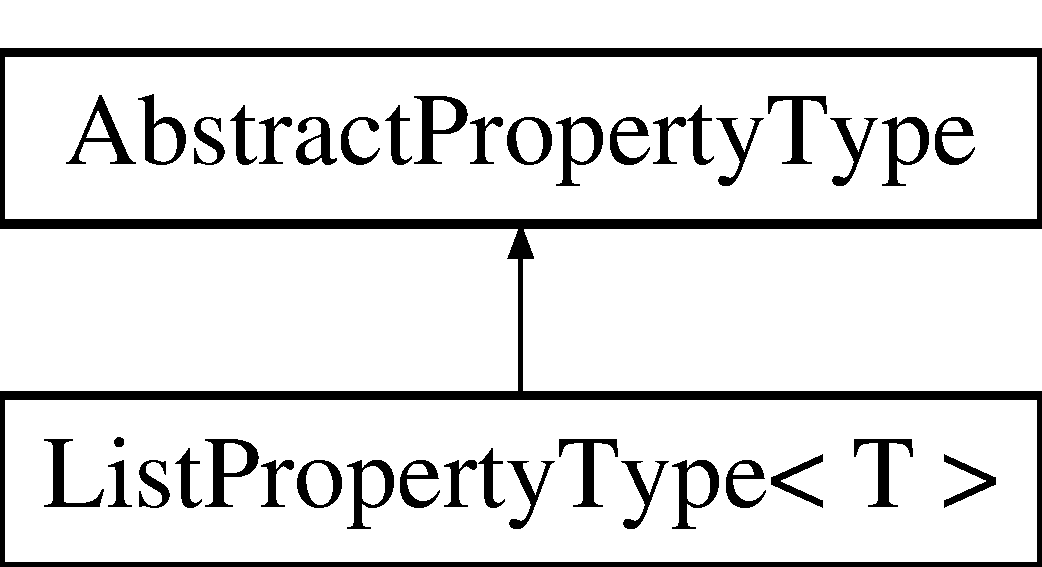
\includegraphics[height=2.000000cm]{classListPropertyType}
\end{center}
\end{figure}
\subsection*{Public Member Functions}
\begin{DoxyCompactItemize}
\item 
\hypertarget{classListPropertyType_a5e6f35179b6e7c79cf7dd831db1f5ffd}{{\bfseries List\-Property\-Type} (std\-::string property\-Name)}\label{classListPropertyType_a5e6f35179b6e7c79cf7dd831db1f5ffd}

\item 
\hypertarget{classListPropertyType_a72d99362f99900b292e0a8e78e9d2d2f}{{\bfseries List\-Property\-Type} (std\-::string property\-Name, \hyperlink{classAbstractPropertyType}{Abstract\-Property\-Type} $\ast$value)}\label{classListPropertyType_a72d99362f99900b292e0a8e78e9d2d2f}

\item 
\hypertarget{classListPropertyType_a97b74dbcac25f0ea6610bfea24916ef6}{{\bfseries List\-Property\-Type} (\hyperlink{classListPropertyType}{List\-Property\-Type} \&other)}\label{classListPropertyType_a97b74dbcac25f0ea6610bfea24916ef6}

\item 
void \hyperlink{classListPropertyType_a18501d9e46af59ee269c6c6473ff0c99}{append} (\hyperlink{classAbstractPropertyType}{Abstract\-Property\-Type} $\ast$property)
\item 
\hypertarget{classListPropertyType_a03589ed61592cf3061542b73abf00c67}{uint {\bfseries count} ()}\label{classListPropertyType_a03589ed61592cf3061542b73abf00c67}

\item 
\hypertarget{classListPropertyType_a2b4d928c8fa6c7317a31d4aa376908d1}{\hyperlink{classAbstractPropertyType}{Abstract\-Property\-Type} $\ast$ {\bfseries copy} ()}\label{classListPropertyType_a2b4d928c8fa6c7317a31d4aa376908d1}

\item 
\hypertarget{classListPropertyType_a7c0f0a4ab1d1ceaf4d7abfbdade7f5ea}{std\-::string {\bfseries to\-String} () const }\label{classListPropertyType_a7c0f0a4ab1d1ceaf4d7abfbdade7f5ea}

\item 
\hypertarget{classListPropertyType_aa49d1bc6968d7201b4d836b5049133f0}{void {\bfseries from\-String} (std\-::string str)}\label{classListPropertyType_aa49d1bc6968d7201b4d836b5049133f0}

\item 
\hypertarget{classListPropertyType_ab0a0e192757158cd9901becacbafdb41}{G\-Variant $\ast$ {\bfseries to\-Variant} ()}\label{classListPropertyType_ab0a0e192757158cd9901becacbafdb41}

\item 
void \hyperlink{classListPropertyType_aa76b2385816ce8a12982109d632b6b93}{from\-Variant} (G\-Variant $\ast$v)
\item 
\hypertarget{classListPropertyType_a764a0d0ab730b7821514d7158e1df05b}{std\-::list$<$ \hyperlink{classAbstractPropertyType}{Abstract\-Property\-Type} $\ast$ $>$ {\bfseries list} ()}\label{classListPropertyType_a764a0d0ab730b7821514d7158e1df05b}

\end{DoxyCompactItemize}
\subsection*{Additional Inherited Members}


\subsection{Member Function Documentation}
\hypertarget{classListPropertyType_a18501d9e46af59ee269c6c6473ff0c99}{\index{List\-Property\-Type@{List\-Property\-Type}!append@{append}}
\index{append@{append}!ListPropertyType@{List\-Property\-Type}}
\subsubsection[{append}]{\setlength{\rightskip}{0pt plus 5cm}template$<$class T $>$ void {\bf List\-Property\-Type}$<$ T $>$\-::append (
\begin{DoxyParamCaption}
\item[{{\bf Abstract\-Property\-Type} $\ast$}]{property}
\end{DoxyParamCaption}
)\hspace{0.3cm}{\ttfamily [inline]}}}\label{classListPropertyType_a18501d9e46af59ee269c6c6473ff0c99}
append -\/ appends a property to the list \begin{DoxyItemize}
\item property -\/ property to be appended. Property will be copied and owned by \hyperlink{classListPropertyType}{List\-Property\-Type}. You are responsible for freeing property after append is called. \end{DoxyItemize}
\hypertarget{classListPropertyType_aa76b2385816ce8a12982109d632b6b93}{\index{List\-Property\-Type@{List\-Property\-Type}!from\-Variant@{from\-Variant}}
\index{from\-Variant@{from\-Variant}!ListPropertyType@{List\-Property\-Type}}
\subsubsection[{from\-Variant}]{\setlength{\rightskip}{0pt plus 5cm}template$<$class T $>$ void {\bf List\-Property\-Type}$<$ T $>$\-::from\-Variant (
\begin{DoxyParamCaption}
\item[{G\-Variant $\ast$}]{v}
\end{DoxyParamCaption}
)\hspace{0.3cm}{\ttfamily [inline]}, {\ttfamily [virtual]}}}\label{classListPropertyType_aa76b2385816ce8a12982109d632b6b93}
T\-O\-D\-O\-: fill this in 

Implements \hyperlink{classAbstractPropertyType}{Abstract\-Property\-Type}.



The documentation for this class was generated from the following file\-:\begin{DoxyCompactItemize}
\item 
/home/tripzero/src/automotive-\/message-\/broker/lib/abstractpropertytype.\-h\end{DoxyCompactItemize}

\hypertarget{classMapPropertyType}{\section{Map\-Property\-Type$<$ T, N $>$ Class Template Reference}
\label{classMapPropertyType}\index{Map\-Property\-Type$<$ T, N $>$@{Map\-Property\-Type$<$ T, N $>$}}
}
Inheritance diagram for Map\-Property\-Type$<$ T, N $>$\-:\begin{figure}[H]
\begin{center}
\leavevmode
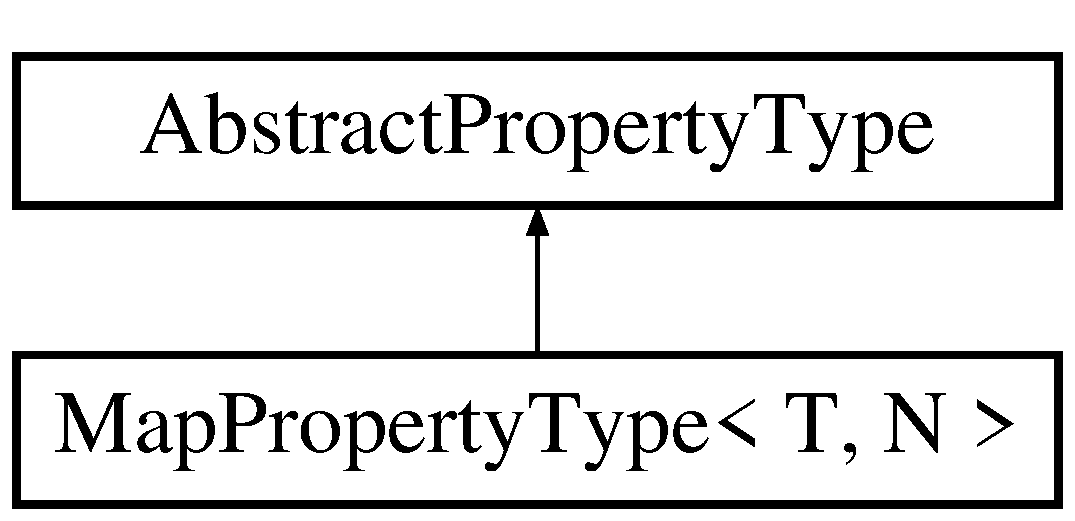
\includegraphics[height=2.000000cm]{classMapPropertyType}
\end{center}
\end{figure}
\subsection*{Public Member Functions}
\begin{DoxyCompactItemize}
\item 
\hypertarget{classMapPropertyType_aa1a20f8411d6642e6d9d16d2c49e8616}{{\bfseries Map\-Property\-Type} (std\-::string property\-Name)}\label{classMapPropertyType_aa1a20f8411d6642e6d9d16d2c49e8616}

\item 
\hypertarget{classMapPropertyType_a204d5a2ef375b9f96badbac88e90c399}{void {\bfseries append} (T key, N value)}\label{classMapPropertyType_a204d5a2ef375b9f96badbac88e90c399}

\item 
\hypertarget{classMapPropertyType_abcc0f1c2cd4faff2859420f90dd67cad}{\hyperlink{classAbstractPropertyType}{Abstract\-Property\-Type} $\ast$ {\bfseries copy} ()}\label{classMapPropertyType_abcc0f1c2cd4faff2859420f90dd67cad}

\item 
\hypertarget{classMapPropertyType_a662d25c3cd9e1732f0cd2dabd38c1bcd}{std\-::string {\bfseries to\-String} () const }\label{classMapPropertyType_a662d25c3cd9e1732f0cd2dabd38c1bcd}

\item 
\hypertarget{classMapPropertyType_aae407d89167cad46b2ab63971d1e68f5}{void {\bfseries from\-String} (std\-::string str)}\label{classMapPropertyType_aae407d89167cad46b2ab63971d1e68f5}

\item 
\hypertarget{classMapPropertyType_a0dfca18093e88f7ae8788bf1ce852109}{G\-Variant $\ast$ {\bfseries to\-Variant} ()}\label{classMapPropertyType_a0dfca18093e88f7ae8788bf1ce852109}

\item 
void \hyperlink{classMapPropertyType_a9038e06690c5d3718be1aadb6752bfbe}{from\-Variant} (G\-Variant $\ast$variant)
\item 
\hypertarget{classMapPropertyType_abfecbe98555c77f13bab01892ea143a7}{void {\bfseries set\-Map} (std\-::map$<$ T, N $>$ m)}\label{classMapPropertyType_abfecbe98555c77f13bab01892ea143a7}

\end{DoxyCompactItemize}
\subsection*{Additional Inherited Members}


\subsection{Member Function Documentation}
\hypertarget{classMapPropertyType_a9038e06690c5d3718be1aadb6752bfbe}{\index{Map\-Property\-Type@{Map\-Property\-Type}!from\-Variant@{from\-Variant}}
\index{from\-Variant@{from\-Variant}!MapPropertyType@{Map\-Property\-Type}}
\subsubsection[{from\-Variant}]{\setlength{\rightskip}{0pt plus 5cm}template$<$class T, class N$>$ void {\bf Map\-Property\-Type}$<$ T, N $>$\-::from\-Variant (
\begin{DoxyParamCaption}
\item[{G\-Variant $\ast$}]{variant}
\end{DoxyParamCaption}
)\hspace{0.3cm}{\ttfamily [inline]}, {\ttfamily [virtual]}}}\label{classMapPropertyType_a9038e06690c5d3718be1aadb6752bfbe}
T\-O\-D\-O\-: fill this in 

Implements \hyperlink{classAbstractPropertyType}{Abstract\-Property\-Type}.



The documentation for this class was generated from the following file\-:\begin{DoxyCompactItemize}
\item 
/home/kev/src/automotive-\/message-\/broker/lib/mappropertytype.\-hpp\end{DoxyCompactItemize}

\hypertarget{classPropertyInfo}{\section{Property\+Info Class Reference}
\label{classPropertyInfo}\index{Property\+Info@{Property\+Info}}
}
\subsection*{Public Member Functions}
\begin{DoxyCompactItemize}
\item 
\hyperlink{classPropertyInfo_aec9353196a1c2bbebd516e0f548e15ad}{Property\+Info} ()
\item 
\hyperlink{classPropertyInfo_aca0b540318420cc779cba04c9fc49b70}{Property\+Info} (uint update\+Freq, Zone\+::\+Zone\+List zones\+List)
\item 
uint \hyperlink{classPropertyInfo_a8e6740dabbdea52c6b0900549c109963}{update\+Frequency} ()
\item 
Zone\+::\+Zone\+List \hyperlink{classPropertyInfo_ab0743a56cb3e6c0ed9dc959f3e388bee}{zones} ()
\item 
bool \hyperlink{classPropertyInfo_a574538766c305b7303a0d5721a0fd0d1}{is\+Valid} ()
\end{DoxyCompactItemize}
\subsection*{Static Public Member Functions}
\begin{DoxyCompactItemize}
\item 
static \hyperlink{classPropertyInfo}{Property\+Info} \hyperlink{classPropertyInfo_a5a3e9a1198ac54a40b1f3ae009bb1397}{invalid} ()
\end{DoxyCompactItemize}


\subsection{Constructor \& Destructor Documentation}
\hypertarget{classPropertyInfo_aec9353196a1c2bbebd516e0f548e15ad}{\index{Property\+Info@{Property\+Info}!Property\+Info@{Property\+Info}}
\index{Property\+Info@{Property\+Info}!Property\+Info@{Property\+Info}}
\subsubsection[{Property\+Info}]{\setlength{\rightskip}{0pt plus 5cm}Property\+Info\+::\+Property\+Info (
\begin{DoxyParamCaption}
{}
\end{DoxyParamCaption}
)\hspace{0.3cm}{\ttfamily [inline]}}}\label{classPropertyInfo_aec9353196a1c2bbebd516e0f548e15ad}
\hyperlink{classPropertyInfo}{Property\+Info} \hypertarget{classPropertyInfo_aca0b540318420cc779cba04c9fc49b70}{\index{Property\+Info@{Property\+Info}!Property\+Info@{Property\+Info}}
\index{Property\+Info@{Property\+Info}!Property\+Info@{Property\+Info}}
\subsubsection[{Property\+Info}]{\setlength{\rightskip}{0pt plus 5cm}Property\+Info\+::\+Property\+Info (
\begin{DoxyParamCaption}
\item[{uint}]{update\+Freq, }
\item[{Zone\+::\+Zone\+List}]{zones\+List}
\end{DoxyParamCaption}
)\hspace{0.3cm}{\ttfamily [inline]}}}\label{classPropertyInfo_aca0b540318420cc779cba04c9fc49b70}
\hyperlink{classPropertyInfo}{Property\+Info} \begin{DoxyItemize}
\item update\+Frequency \item zones\+List \end{DoxyItemize}


\subsection{Member Function Documentation}
\hypertarget{classPropertyInfo_a5a3e9a1198ac54a40b1f3ae009bb1397}{\index{Property\+Info@{Property\+Info}!invalid@{invalid}}
\index{invalid@{invalid}!Property\+Info@{Property\+Info}}
\subsubsection[{invalid}]{\setlength{\rightskip}{0pt plus 5cm}static {\bf Property\+Info} Property\+Info\+::invalid (
\begin{DoxyParamCaption}
{}
\end{DoxyParamCaption}
)\hspace{0.3cm}{\ttfamily [inline]}, {\ttfamily [static]}}}\label{classPropertyInfo_a5a3e9a1198ac54a40b1f3ae009bb1397}
\hyperlink{classPropertyInfo_a5a3e9a1198ac54a40b1f3ae009bb1397}{invalid()} returns instance of \hyperlink{classPropertyInfo}{Property\+Info} that isn't valid \hypertarget{classPropertyInfo_a574538766c305b7303a0d5721a0fd0d1}{\index{Property\+Info@{Property\+Info}!is\+Valid@{is\+Valid}}
\index{is\+Valid@{is\+Valid}!Property\+Info@{Property\+Info}}
\subsubsection[{is\+Valid}]{\setlength{\rightskip}{0pt plus 5cm}bool Property\+Info\+::is\+Valid (
\begin{DoxyParamCaption}
{}
\end{DoxyParamCaption}
)\hspace{0.3cm}{\ttfamily [inline]}}}\label{classPropertyInfo_a574538766c305b7303a0d5721a0fd0d1}
is\+Valid returns whether this \hyperlink{classPropertyInfo}{Property\+Info} is valid

default when you construct a \hyperlink{classPropertyInfo}{Property\+Info} is false \hypertarget{classPropertyInfo_a8e6740dabbdea52c6b0900549c109963}{\index{Property\+Info@{Property\+Info}!update\+Frequency@{update\+Frequency}}
\index{update\+Frequency@{update\+Frequency}!Property\+Info@{Property\+Info}}
\subsubsection[{update\+Frequency}]{\setlength{\rightskip}{0pt plus 5cm}uint Property\+Info\+::update\+Frequency (
\begin{DoxyParamCaption}
{}
\end{DoxyParamCaption}
)\hspace{0.3cm}{\ttfamily [inline]}}}\label{classPropertyInfo_a8e6740dabbdea52c6b0900549c109963}
update\+Frequency Maximum times per second a property is expected to update. \hypertarget{classPropertyInfo_ab0743a56cb3e6c0ed9dc959f3e388bee}{\index{Property\+Info@{Property\+Info}!zones@{zones}}
\index{zones@{zones}!Property\+Info@{Property\+Info}}
\subsubsection[{zones}]{\setlength{\rightskip}{0pt plus 5cm}Zone\+::\+Zone\+List Property\+Info\+::zones (
\begin{DoxyParamCaption}
{}
\end{DoxyParamCaption}
)\hspace{0.3cm}{\ttfamily [inline]}}}\label{classPropertyInfo_ab0743a56cb3e6c0ed9dc959f3e388bee}
zones Number of different zones supported by this property. 

The documentation for this class was generated from the following file\+:\begin{DoxyCompactItemize}
\item 
/home/kev/src/automotive-\/message-\/broker/lib/propertyinfo.\+hpp\end{DoxyCompactItemize}

\hypertarget{classamb_1_1Queue}{\section{amb\-:\-:Queue$<$ T, Pred $>$ Class Template Reference}
\label{classamb_1_1Queue}\index{amb\-::\-Queue$<$ T, Pred $>$@{amb\-::\-Queue$<$ T, Pred $>$}}
}
\subsection*{Public Member Functions}
\begin{DoxyCompactItemize}
\item 
\hypertarget{classamb_1_1Queue_ab3896fe943b628902a5148a4fa7cb61a}{int {\bfseries count} ()}\label{classamb_1_1Queue_ab3896fe943b628902a5148a4fa7cb61a}

\item 
\hypertarget{classamb_1_1Queue_ac837c984d97965ab1f584462441509cc}{T {\bfseries pop} ()}\label{classamb_1_1Queue_ac837c984d97965ab1f584462441509cc}

\item 
\hypertarget{classamb_1_1Queue_a723ec2204cc96eb51d1cbda721000503}{virtual void {\bfseries append} (T item)}\label{classamb_1_1Queue_a723ec2204cc96eb51d1cbda721000503}

\item 
\hypertarget{classamb_1_1Queue_a67967c4d70037e3b02365bdcce4dbb52}{void {\bfseries remove} (T item)}\label{classamb_1_1Queue_a67967c4d70037e3b02365bdcce4dbb52}

\end{DoxyCompactItemize}
\subsection*{Protected Attributes}
\begin{DoxyCompactItemize}
\item 
\hypertarget{classamb_1_1Queue_a8ac352d50bc26d93de0340bd16896a35}{std\-::mutex {\bfseries mutex}}\label{classamb_1_1Queue_a8ac352d50bc26d93de0340bd16896a35}

\item 
\hypertarget{classamb_1_1Queue_a3d3bd5ab679821f93ffcd51270ebc41c}{std\-::unordered\-\_\-set$<$ T, \\*
std\-::hash$<$ T $>$, Pred $>$ {\bfseries m\-Queue}}\label{classamb_1_1Queue_a3d3bd5ab679821f93ffcd51270ebc41c}

\end{DoxyCompactItemize}


The documentation for this class was generated from the following file\-:\begin{DoxyCompactItemize}
\item 
/home/tripzero/src/automotive-\/message-\/broker/lib/asyncqueue.\-hpp\end{DoxyCompactItemize}

\hypertarget{classStringPropertyType}{\section{String\-Property\-Type Class Reference}
\label{classStringPropertyType}\index{String\-Property\-Type@{String\-Property\-Type}}
}
Inheritance diagram for String\-Property\-Type\-:\begin{figure}[H]
\begin{center}
\leavevmode
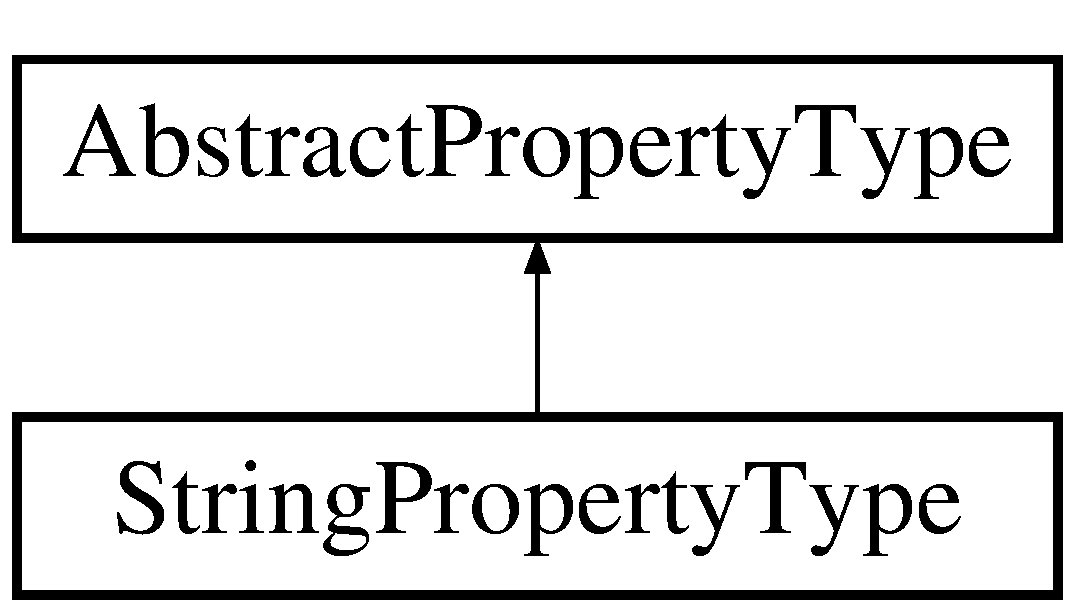
\includegraphics[height=2.000000cm]{classStringPropertyType}
\end{center}
\end{figure}
\subsection*{Public Member Functions}
\begin{DoxyCompactItemize}
\item 
\hypertarget{classStringPropertyType_ac9474db13442001b615cb29b889844eb}{{\bfseries String\-Property\-Type} (std\-::string property\-Name)}\label{classStringPropertyType_ac9474db13442001b615cb29b889844eb}

\item 
\hypertarget{classStringPropertyType_a071f749092ee76790fb508f0ea8c974a}{{\bfseries String\-Property\-Type} (std\-::string property\-Name, std\-::string val)}\label{classStringPropertyType_a071f749092ee76790fb508f0ea8c974a}

\item 
\hypertarget{classStringPropertyType_a221e152eec4bfa2bab6e063dd7eb2108}{{\bfseries String\-Property\-Type} (\hyperlink{classStringPropertyType}{String\-Property\-Type} const \&other)}\label{classStringPropertyType_a221e152eec4bfa2bab6e063dd7eb2108}

\item 
\hypertarget{classStringPropertyType_a2eb25280c4494ff5f9aca137bf5040c7}{\hyperlink{classStringPropertyType}{String\-Property\-Type} \& {\bfseries operator=} (\hyperlink{classStringPropertyType}{String\-Property\-Type} const \&other)}\label{classStringPropertyType_a2eb25280c4494ff5f9aca137bf5040c7}

\item 
\hypertarget{classStringPropertyType_ad9dd60fcfd9fd3ebaa578815c8d552fe}{void {\bfseries from\-String} (std\-::string val)}\label{classStringPropertyType_ad9dd60fcfd9fd3ebaa578815c8d552fe}

\item 
\hypertarget{classStringPropertyType_a15866eb8e3ee9e1be587740f64353d57}{\hyperlink{classAbstractPropertyType}{Abstract\-Property\-Type} $\ast$ {\bfseries copy} ()}\label{classStringPropertyType_a15866eb8e3ee9e1be587740f64353d57}

\item 
\hypertarget{classStringPropertyType_afb461a0a918e23e66880d0c8d2180b35}{std\-::string {\bfseries to\-String} () const }\label{classStringPropertyType_afb461a0a918e23e66880d0c8d2180b35}

\item 
\hypertarget{classStringPropertyType_a1ec1ba3797194880a1e7576bd3695a28}{G\-Variant $\ast$ {\bfseries to\-Variant} ()}\label{classStringPropertyType_a1ec1ba3797194880a1e7576bd3695a28}

\item 
\hypertarget{classStringPropertyType_ad4a1e7db1f6b381ab956eb70afd1509e}{void {\bfseries from\-Variant} (G\-Variant $\ast$v)}\label{classStringPropertyType_ad4a1e7db1f6b381ab956eb70afd1509e}

\end{DoxyCompactItemize}
\subsection*{Additional Inherited Members}


The documentation for this class was generated from the following file\-:\begin{DoxyCompactItemize}
\item 
/home/kev/src/automotive-\/message-\/broker/lib/abstractpropertytype.\-h\end{DoxyCompactItemize}

\hypertarget{structamb_1_1traits}{\section{amb\-:\-:traits$<$ T $>$ Struct Template Reference}
\label{structamb_1_1traits}\index{amb\-::traits$<$ T $>$@{amb\-::traits$<$ T $>$}}
}


The documentation for this struct was generated from the following file\-:\begin{DoxyCompactItemize}
\item 
/home/tripzero/src/automotive-\/message-\/broker/lib/superptr.\-hpp\end{DoxyCompactItemize}

\hypertarget{structamb_1_1traits_3_01gchar_01_4}{\section{amb\-:\-:traits$<$ gchar $>$ Struct Template Reference}
\label{structamb_1_1traits_3_01gchar_01_4}\index{amb\-::traits$<$ gchar $>$@{amb\-::traits$<$ gchar $>$}}
}
\subsection*{Classes}
\begin{DoxyCompactItemize}
\item 
struct \hyperlink{structamb_1_1traits_3_01gchar_01_4_1_1delete__functor}{delete\-\_\-functor}
\end{DoxyCompactItemize}


The documentation for this struct was generated from the following file\-:\begin{DoxyCompactItemize}
\item 
/home/tripzero/src/automotive-\/message-\/broker/lib/superptr.\-hpp\end{DoxyCompactItemize}

\hypertarget{structamb_1_1traits_3_01GDBusProxy_01_4}{\section{amb\-:\-:traits$<$ G\-D\-Bus\-Proxy $>$ Struct Template Reference}
\label{structamb_1_1traits_3_01GDBusProxy_01_4}\index{amb\-::traits$<$ G\-D\-Bus\-Proxy $>$@{amb\-::traits$<$ G\-D\-Bus\-Proxy $>$}}
}
\subsection*{Classes}
\begin{DoxyCompactItemize}
\item 
struct \hyperlink{structamb_1_1traits_3_01GDBusProxy_01_4_1_1delete__functor}{delete\-\_\-functor}
\end{DoxyCompactItemize}


The documentation for this struct was generated from the following file\-:\begin{DoxyCompactItemize}
\item 
/home/tripzero/src/automotive-\/message-\/broker/lib/superptr.\-hpp\end{DoxyCompactItemize}

\hypertarget{structamb_1_1traits_3_01GError_01_4}{\section{amb\+:\+:traits$<$ G\+Error $>$ Struct Template Reference}
\label{structamb_1_1traits_3_01GError_01_4}\index{amb\+::traits$<$ G\+Error $>$@{amb\+::traits$<$ G\+Error $>$}}
}
\subsection*{Classes}
\begin{DoxyCompactItemize}
\item 
struct \hyperlink{structamb_1_1traits_3_01GError_01_4_1_1delete__functor}{delete\+\_\+functor}
\end{DoxyCompactItemize}


The documentation for this struct was generated from the following file\+:\begin{DoxyCompactItemize}
\item 
/home/kev/src/automotive-\/message-\/broker/lib/superptr.\+hpp\end{DoxyCompactItemize}

\hypertarget{structamb_1_1traits_3_01GVariant_01_4}{\section{amb\+:\+:traits$<$ G\+Variant $>$ Struct Template Reference}
\label{structamb_1_1traits_3_01GVariant_01_4}\index{amb\+::traits$<$ G\+Variant $>$@{amb\+::traits$<$ G\+Variant $>$}}
}
\subsection*{Classes}
\begin{DoxyCompactItemize}
\item 
struct \hyperlink{structamb_1_1traits_3_01GVariant_01_4_1_1delete__functor}{delete\+\_\+functor}
\end{DoxyCompactItemize}


The documentation for this struct was generated from the following file\+:\begin{DoxyCompactItemize}
\item 
/home/kev/src/automotive-\/message-\/broker/lib/superptr.\+hpp\end{DoxyCompactItemize}

\hypertarget{structamb_1_1traits_3_01GVariantIter_01_4}{\section{amb\+:\+:traits$<$ G\+Variant\+Iter $>$ Struct Template Reference}
\label{structamb_1_1traits_3_01GVariantIter_01_4}\index{amb\+::traits$<$ G\+Variant\+Iter $>$@{amb\+::traits$<$ G\+Variant\+Iter $>$}}
}
\subsection*{Classes}
\begin{DoxyCompactItemize}
\item 
struct \hyperlink{structamb_1_1traits_3_01GVariantIter_01_4_1_1delete__functor}{delete\+\_\+functor}
\end{DoxyCompactItemize}


The documentation for this struct was generated from the following file\+:\begin{DoxyCompactItemize}
\item 
/home/kev/src/automotive-\/message-\/broker/lib/superptr.\+hpp\end{DoxyCompactItemize}

\hypertarget{classVehicleProperty}{\section{Vehicle\-Property Class Reference}
\label{classVehicleProperty}\index{Vehicle\-Property@{Vehicle\-Property}}
}
\subsection*{Public Types}
\begin{DoxyCompactItemize}
\item 
\hypertarget{classVehicleProperty_acf303d050168f571e838813f3e6042d1}{typedef std\-::string {\bfseries Property}}\label{classVehicleProperty_acf303d050168f571e838813f3e6042d1}

\item 
typedef std\-::function\\*
$<$ \hyperlink{classAbstractPropertyType}{Abstract\-Property\-Type} $\ast$(void)$>$ \hyperlink{classVehicleProperty_a6fdd075ce5b867b571020fcdc723ddcf}{Property\-Type\-Factory\-Callback}
\begin{DoxyCompactList}\small\item\em Property\-Type\-Factory\-Callback callback used to construct a \hyperlink{classAbstractPropertyType}{Abstract\-Property\-Type} for a property. \end{DoxyCompactList}\end{DoxyCompactItemize}
\subsection*{Public Member Functions}
\begin{DoxyCompactItemize}
\item 
\hyperlink{classVehicleProperty_a768a0be8079ce3e1645cdc259a84adf7}{P\-R\-O\-P\-E\-R\-T\-Y\-T\-Y\-P\-E} (\hyperlink{classVehicleProperty_ae486d9ea26918460822086b797018800}{Transmission\-Shift\-Position}, Transmission\-Shift\-Position\-Type, \hyperlink{classBasicPropertyType}{Basic\-Property\-Type}$<$ Transmission\-::\-Transmission\-Positions $>$, Transmission\-::\-Transmission\-Positions) static const Property Transmission\-Gear\-Position
\item 
\hypertarget{classVehicleProperty_af9df28b1bc1bef05442b6b1cce40c80e}{{\bfseries P\-R\-O\-P\-E\-R\-T\-Y\-T\-Y\-P\-E} (Transmission\-Gear\-Position, Transmission\-Gear\-Position\-Type, \hyperlink{classBasicPropertyType}{Basic\-Property\-Type}$<$ Transmission\-::\-Transmission\-Positions $>$, Transmission\-::\-Transmission\-Positions) static const Property Transmission\-Mode}\label{classVehicleProperty_af9df28b1bc1bef05442b6b1cce40c80e}

\item 
\hyperlink{classVehicleProperty_ac6527b3ae7e7697c2a23c5903b471172}{P\-R\-O\-P\-E\-R\-T\-Y\-T\-Y\-P\-E} (Transmission\-Mode, Transmission\-Mode\-Type, \hyperlink{classBasicPropertyType}{Basic\-Property\-Type}$<$ Transmission\-::\-Mode $>$, Transmission\-::\-Mode) static const Property Throttle\-Position
\end{DoxyCompactItemize}
\subsection*{Static Public Member Functions}
\begin{DoxyCompactItemize}
\item 
\hypertarget{classVehicleProperty_a528c8e2ee75036f6e50c0121f4184fa2}{static void \hyperlink{classVehicleProperty_a528c8e2ee75036f6e50c0121f4184fa2}{factory} ()}\label{classVehicleProperty_a528c8e2ee75036f6e50c0121f4184fa2}

\begin{DoxyCompactList}\small\item\em factory constructs a static instance of \hyperlink{classVehicleProperty}{Vehicle\-Property}. This should be called once before \hyperlink{classVehicleProperty}{Vehicle\-Property} is used in the app \end{DoxyCompactList}\item 
static std\-::list\\*
$<$ Vehicle\-Property\-::\-Property $>$ \hyperlink{classVehicleProperty_aa238272767b6b4101b9bef14bf09631b}{capabilities} ()
\begin{DoxyCompactList}\small\item\em capabilities \end{DoxyCompactList}\item 
static std\-::list\\*
$<$ Vehicle\-Property\-::\-Property $>$ \hyperlink{classVehicleProperty_a5a9afad3f68db690652b80cfccdffc66}{custom\-Properties} ()
\begin{DoxyCompactList}\small\item\em custom\-Properties \end{DoxyCompactList}\item 
\hypertarget{classVehicleProperty_a60e654875a0d5901af8ab2d3dc596472}{static \hyperlink{classAbstractPropertyType}{Abstract\-Property\-Type} $\ast$ \hyperlink{classVehicleProperty_a60e654875a0d5901af8ab2d3dc596472}{get\-Property\-Type\-For\-Property\-Name\-Value} (Property name, std\-::string value=\char`\"{}\char`\"{})}\label{classVehicleProperty_a60e654875a0d5901af8ab2d3dc596472}

\begin{DoxyCompactList}\small\item\em get\-Property\-Type\-For\-Property\-Name\-Value returns an Abstract\-Property\-Type$\ast$ for the property name with the value specified by 'value'. Ownership of the returned Abstract\-Property\-Type$\ast$ is transfered to the caller. \end{DoxyCompactList}\item 
\hypertarget{classVehicleProperty_aec55cb2758688c0e92dc53f67b320208}{static bool {\bfseries register\-Property} (Property name, \hyperlink{classVehicleProperty_a6fdd075ce5b867b571020fcdc723ddcf}{Property\-Type\-Factory\-Callback} \hyperlink{classVehicleProperty_a528c8e2ee75036f6e50c0121f4184fa2}{factory})}\label{classVehicleProperty_aec55cb2758688c0e92dc53f67b320208}

\end{DoxyCompactItemize}
\subsection*{Static Public Attributes}
\begin{DoxyCompactItemize}
\item 
static const Property \hyperlink{classVehicleProperty_ae013e9c1f3fb57d646211d3e6bb4ca9e}{No\-Value} = \char`\"{}No\-Value\char`\"{}
\begin{DoxyCompactList}\small\item\em Various property types\-: \end{DoxyCompactList}\item 
\hypertarget{classVehicleProperty_af457ed63f945a7f6b4e074f3ba8b904f}{static const Property {\bfseries Vehicle\-Speed} = \char`\"{}Vehicle\-Speed\char`\"{}}\label{classVehicleProperty_af457ed63f945a7f6b4e074f3ba8b904f}

\item 
static const Property \hyperlink{classVehicleProperty_a7949fe3d031814fc2644de14f8cec9a0}{Engine\-Speed} = \char`\"{}Engine\-Speed\char`\"{}
\item 
static const Property \hyperlink{classVehicleProperty_ae486d9ea26918460822086b797018800}{Transmission\-Shift\-Position} = \char`\"{}Transmission\-Shift\-Position\char`\"{}
\item 
static const Property \hyperlink{classVehicleProperty_ad4f1ec038bee5ef30fbf8308aaba2794}{Wheel\-Brake} = \char`\"{}Wheel\-Brake\char`\"{}
\item 
\hypertarget{classVehicleProperty_a617cc19f62d99f7f72a047d5066dcd96}{static const Property {\bfseries Wheel\-Brake\-Pressure} = \char`\"{}Wheel\-Brake\-Pressure\char`\"{}}\label{classVehicleProperty_a617cc19f62d99f7f72a047d5066dcd96}

\item 
static const Property \hyperlink{classVehicleProperty_aba4832663e4f850acbcf09c7cfbc6959}{Steering\-Wheel\-Angle} = \char`\"{}Steering\-Wheel\-Angle\char`\"{}
\item 
static const Property \hyperlink{classVehicleProperty_a0aae609c370a46a92dc52a31d2cc0310}{Turn\-Signal} = \char`\"{}Turn\-Signal\char`\"{}
\item 
static const Property \hyperlink{classVehicleProperty_acdca2ca718fd392c7ad9b8adc817baec}{Clutch\-Status} = \char`\"{}Clutch\-Status\char`\"{}
\item 
static const Property \hyperlink{classVehicleProperty_ab7fad273c7149dbd338f53f2536aca26}{Engine\-Oil\-Pressure} = \char`\"{}Engine\-Oil\-Pressure\char`\"{}
\item 
static const Property \hyperlink{classVehicleProperty_ae4f240ad9cecbbb9d0cb3a615865b60a}{Engine\-Coolant\-Temperature} = \char`\"{}Engine\-Coolant\-Temperature\char`\"{}
\item 
static const Property \hyperlink{classVehicleProperty_a8b9faaa1094c2d162ed171a3063b7ffc}{Machine\-Gun\-Turret\-Status} = \char`\"{}Machine\-Gun\-Turret\-Status\char`\"{}
\item 
static const Property \hyperlink{classVehicleProperty_a94eac12d319850190e9ece93690517f7}{Acceleration\-X} = \char`\"{}Acceleration\-X\char`\"{}
\item 
static const Property \hyperlink{classVehicleProperty_af56803eeb7710aeae2954f4cd9b66cf6}{Acceleration\-Y} = \char`\"{}Acceleration\-Y\char`\"{}
\item 
static const Property \hyperlink{classVehicleProperty_a1ce0b3be3a09d5a96741890d0d67496f}{Acceleration\-Z} = \char`\"{}Acceleration\-Z\char`\"{}
\item 
\hypertarget{classVehicleProperty_aabc6b6b50b8a31bfe197cbd3ae0827a1}{static const Property {\bfseries Mass\-Air\-Flow} = \char`\"{}Mass\-Air\-Flow\char`\"{}}\label{classVehicleProperty_aabc6b6b50b8a31bfe197cbd3ae0827a1}

\item 
static const Property \hyperlink{classVehicleProperty_ab9fa252d209fbd2eb014c4d934d3d615}{Button\-Event} = \char`\"{}Button\-Event\char`\"{}
\item 
static const Property \hyperlink{classVehicleProperty_af4cbbae11228729335c50aa2d1fa2e28}{Air\-Intake\-Temperature} = \char`\"{}Air\-Intake\-Temperature\char`\"{}
\item 
static const Property \hyperlink{classVehicleProperty_a43a70a277b955ae35a9ba795d2052591}{Battery\-Voltage} = \char`\"{}Battery\-Voltage\char`\"{}
\item 
\hypertarget{classVehicleProperty_a3447a00e8ca09d12b208bc7c210a61b8}{static const Property {\bfseries Battery\-Current} = \char`\"{}Battery\-Current\char`\"{}}\label{classVehicleProperty_a3447a00e8ca09d12b208bc7c210a61b8}

\item 
static const Property \hyperlink{classVehicleProperty_adbbb68033f8531903ff3e3024864eef3}{Interior\-Temperature} = \char`\"{}Interior\-Temperature\char`\"{}
\item 
\hypertarget{classVehicleProperty_ad9510186dc9ef236b59743371f093d36}{static const Property {\bfseries Exterior\-Temperature} = \char`\"{}Exterior\-Temperature\char`\"{}}\label{classVehicleProperty_ad9510186dc9ef236b59743371f093d36}

\item 
static const Property \hyperlink{classVehicleProperty_a9d4a610d94b12f139ea00b271804a73f}{Engine\-Oil\-Temperature} = \char`\"{}Engine\-Oil\-Temperature\char`\"{}
\item 
\hypertarget{classVehicleProperty_aeeece192dedcd20cb112dea6905aa80c}{static const Property {\bfseries Engine\-Oil\-Remaining} = \char`\"{}Engine\-Oil\-Remaining\char`\"{}}\label{classVehicleProperty_aeeece192dedcd20cb112dea6905aa80c}

\item 
static const Property \hyperlink{classVehicleProperty_ae72c1c7de185f330862c62dfb9d93a34}{V\-I\-N} = \char`\"{}V\-I\-N\char`\"{}
\item 
static const Property \hyperlink{classVehicleProperty_a32f980d900d97cf94171ea9fa25408e0}{W\-M\-I} = \char`\"{}W\-M\-I\char`\"{}
\item 
static const Property \hyperlink{classVehicleProperty_ac9231c21753a535525d8526889f7a998}{Tire\-Pressure\-Left\-Front} = \char`\"{}Tire\-Pressure\-Left\-Front\char`\"{}
\item 
\hypertarget{classVehicleProperty_ad11bf5a2d63d1b934ab6b33a9f351824}{static const Property {\bfseries Tire\-Pressure\-Right\-Front} = \char`\"{}Tire\-Pressure\-Right\-Front\char`\"{}}\label{classVehicleProperty_ad11bf5a2d63d1b934ab6b33a9f351824}

\item 
\hypertarget{classVehicleProperty_af10c5b8637f549de87ae9da4e0188cf7}{static const Property {\bfseries Tire\-Pressure\-Left\-Rear} = \char`\"{}Tire\-Pressure\-Left\-Rear\char`\"{}}\label{classVehicleProperty_af10c5b8637f549de87ae9da4e0188cf7}

\item 
\hypertarget{classVehicleProperty_aa8f728b02a1ba3e12b28fdde64f4ddf0}{static const Property {\bfseries Tire\-Pressure\-Right\-Rear} = \char`\"{}Tire\-Pressure\-Right\-Rear\char`\"{}}\label{classVehicleProperty_aa8f728b02a1ba3e12b28fdde64f4ddf0}

\item 
static const Property \hyperlink{classVehicleProperty_aed78bc0c777f0850dee1ee878c8d613a}{Tire\-Temperature\-Left\-Front} = \char`\"{}Tire\-Temperature\-Left\-Front\char`\"{}
\item 
\hypertarget{classVehicleProperty_ac5c976a11640f09fa709f13830f69c75}{static const Property {\bfseries Tire\-Temperature\-Right\-Front} = \char`\"{}Tire\-Temperature\-Right\-Front\char`\"{}}\label{classVehicleProperty_ac5c976a11640f09fa709f13830f69c75}

\item 
\hypertarget{classVehicleProperty_abf066893a9d17c252b222d617497578d}{static const Property {\bfseries Tire\-Temperature\-Left\-Rear} = \char`\"{}Tire\-Temperature\-Left\-Rear\char`\"{}}\label{classVehicleProperty_abf066893a9d17c252b222d617497578d}

\item 
\hypertarget{classVehicleProperty_aaf68ca684bd75f1e2d8ac78881701318}{static const Property {\bfseries Tire\-Temperature\-Right\-Rear} = \char`\"{}Tire\-Temperature\-Right\-Rear\char`\"{}}\label{classVehicleProperty_aaf68ca684bd75f1e2d8ac78881701318}

\item 
static const Property \hyperlink{classVehicleProperty_a80cc1f343da6754346e4bcc0cc7ae009}{Vehicle\-Power\-Mode} = \char`\"{}Vehicle\-Power\-Mode\char`\"{}
\item 
\hypertarget{classVehicleProperty_a893b05cb0e292082070458efa6066e91}{static const Property {\bfseries Trip\-Meters} = \char`\"{}Trip\-Meters\char`\"{}}\label{classVehicleProperty_a893b05cb0e292082070458efa6066e91}

\item 
\hypertarget{classVehicleProperty_a3203c1cb22ff3b530a887228096863e5}{static const Property {\bfseries Cruise\-Control\-Active} = \char`\"{}Cruise\-Control\-Active\char`\"{}}\label{classVehicleProperty_a3203c1cb22ff3b530a887228096863e5}

\item 
\hypertarget{classVehicleProperty_a50c00b5a2d7cfd500a1cd7473124c737}{static const Property {\bfseries Cruise\-Control\-Speed} = \char`\"{}Cruise\-Control\-Speed\char`\"{}}\label{classVehicleProperty_a50c00b5a2d7cfd500a1cd7473124c737}

\item 
\hypertarget{classVehicleProperty_ae98356a8b49f28837a94b13094156e90}{static const Property {\bfseries Light\-Head} = \char`\"{}Light\-Head\char`\"{}}\label{classVehicleProperty_ae98356a8b49f28837a94b13094156e90}

\item 
\hypertarget{classVehicleProperty_a73cfc2a3afd2dc81f495936dfcf46793}{static const Property {\bfseries Light\-Right\-Turn} = \char`\"{}Light\-Right\-Turn\char`\"{}}\label{classVehicleProperty_a73cfc2a3afd2dc81f495936dfcf46793}

\item 
\hypertarget{classVehicleProperty_a4430db4d7c36d7d047766d88f9fc977c}{static const Property {\bfseries Light\-Left\-Turn} = \char`\"{}Light\-Left\-Turn\char`\"{}}\label{classVehicleProperty_a4430db4d7c36d7d047766d88f9fc977c}

\item 
\hypertarget{classVehicleProperty_aa4f2ae234bd0d045b95cf9980e980dd5}{static const Property {\bfseries Light\-Brake} = \char`\"{}Light\-Brake\char`\"{}}\label{classVehicleProperty_aa4f2ae234bd0d045b95cf9980e980dd5}

\item 
\hypertarget{classVehicleProperty_a6eb38fc244331a26b487f7f9beb69b0c}{static const Property {\bfseries Light\-Fog} = \char`\"{}Light\-Fog\char`\"{}}\label{classVehicleProperty_a6eb38fc244331a26b487f7f9beb69b0c}

\item 
\hypertarget{classVehicleProperty_a0d3992f2e0e50bb74baa5e670f6111f0}{static const Property {\bfseries Light\-Hazard} = \char`\"{}Light\-Hazard\char`\"{}}\label{classVehicleProperty_a0d3992f2e0e50bb74baa5e670f6111f0}

\item 
\hypertarget{classVehicleProperty_a144920830af1df5a59433f98ebd29504}{static const Property {\bfseries Light\-Parking} = \char`\"{}Light\-Parking\char`\"{}}\label{classVehicleProperty_a144920830af1df5a59433f98ebd29504}

\item 
\hypertarget{classVehicleProperty_acce36f505d4b0233c753f0d5f568e255}{static const Property {\bfseries Light\-High\-Beam} = \char`\"{}Light\-High\-Beam\char`\"{}}\label{classVehicleProperty_acce36f505d4b0233c753f0d5f568e255}

\item 
\hypertarget{classVehicleProperty_a16b99ec2210fd4ca509a00e59b80f8c0}{static const Property {\bfseries Interior\-Light\-Driver} = \char`\"{}Interior\-Light\-Driver\char`\"{}}\label{classVehicleProperty_a16b99ec2210fd4ca509a00e59b80f8c0}

\item 
\hypertarget{classVehicleProperty_a86c0bb4ab676e06e3c807d90c92e7240}{static const Property {\bfseries Interior\-Light\-Center} = \char`\"{}Interior\-Light\-Center\char`\"{}}\label{classVehicleProperty_a86c0bb4ab676e06e3c807d90c92e7240}

\item 
\hypertarget{classVehicleProperty_af60682429c3b2c7517715801d4ac0f92}{static const Property {\bfseries Interior\-Light\-Passenger} = \char`\"{}Interior\-Light\-Passenger\char`\"{}}\label{classVehicleProperty_af60682429c3b2c7517715801d4ac0f92}

\item 
\hypertarget{classVehicleProperty_a89cb1e6e8dcb7910270c333d79200665}{static const Property {\bfseries Engine\-Load} = \char`\"{}Engine\-Load\char`\"{}}\label{classVehicleProperty_a89cb1e6e8dcb7910270c333d79200665}

\item 
\hypertarget{classVehicleProperty_a69370e86d3520734d83a4c154b533642}{static const Property {\bfseries Horn} = \char`\"{}Horn\char`\"{}}\label{classVehicleProperty_a69370e86d3520734d83a4c154b533642}

\item 
\hypertarget{classVehicleProperty_a9bfbe5beb9e13c8de62c7514b3b22fc9}{static const Property {\bfseries Fuel\-Level} = \char`\"{}Fuel\-Level\char`\"{}}\label{classVehicleProperty_a9bfbe5beb9e13c8de62c7514b3b22fc9}

\item 
\hypertarget{classVehicleProperty_ae0c98c8cbfb6b8553faabfb9d4a42b35}{static const Property {\bfseries Fuel\-Range} = \char`\"{}Fuel\-Range\char`\"{}}\label{classVehicleProperty_ae0c98c8cbfb6b8553faabfb9d4a42b35}

\item 
\hypertarget{classVehicleProperty_afdc1b7b9ecf211d26221b155aef9a35a}{static const Property {\bfseries Fuel\-Consumption} = \char`\"{}Fuel\-Consumption\char`\"{}}\label{classVehicleProperty_afdc1b7b9ecf211d26221b155aef9a35a}

\item 
\hypertarget{classVehicleProperty_af34bb142d87eb300ce82e112598d5376}{static const Property {\bfseries Fuel\-Economy} = \char`\"{}Fuel\-Economy\char`\"{}}\label{classVehicleProperty_af34bb142d87eb300ce82e112598d5376}

\item 
\hypertarget{classVehicleProperty_aa453a0e6b9edee8da30b1f5b9a32edeb}{static const Property {\bfseries Fuel\-Average\-Economy} = \char`\"{}Fuel\-Average\-Economy\char`\"{}}\label{classVehicleProperty_aa453a0e6b9edee8da30b1f5b9a32edeb}

\item 
\hypertarget{classVehicleProperty_a2df3b5ff14ec4a92fba65ad72be7d5b7}{static const Property {\bfseries Fuel\-Type} = \char`\"{}Fuel\-Type\char`\"{}}\label{classVehicleProperty_a2df3b5ff14ec4a92fba65ad72be7d5b7}

\item 
\hypertarget{classVehicleProperty_a574a971800258aa3d53126ec01e85477}{static const Property {\bfseries Fuel\-Position\-Side} = \char`\"{}Fuel\-Position\-Side\char`\"{}}\label{classVehicleProperty_a574a971800258aa3d53126ec01e85477}

\item 
\hypertarget{classVehicleProperty_a490658c5e633ab54a5bbf11b5f38e994}{static const Property {\bfseries Exterior\-Brightness} = \char`\"{}Exterior\-Brightness\char`\"{}}\label{classVehicleProperty_a490658c5e633ab54a5bbf11b5f38e994}

\item 
\hypertarget{classVehicleProperty_a225bcbd3adba51c5d571a086a98f6b4f}{static const Property {\bfseries Latitude} = \char`\"{}Latitude\char`\"{}}\label{classVehicleProperty_a225bcbd3adba51c5d571a086a98f6b4f}

\item 
\hypertarget{classVehicleProperty_ac5565746cd2dfd2e3f8870d8e292b392}{static const Property {\bfseries Longitude} = \char`\"{}Longitude\char`\"{}}\label{classVehicleProperty_ac5565746cd2dfd2e3f8870d8e292b392}

\item 
\hypertarget{classVehicleProperty_a0411474f4450758ba2dbcdc136ef7391}{static const Property {\bfseries Altitude} = \char`\"{}Altitude\char`\"{}}\label{classVehicleProperty_a0411474f4450758ba2dbcdc136ef7391}

\item 
\hypertarget{classVehicleProperty_a89d7508f610bdbbeaaec742ee3d4f656}{static const Property {\bfseries Direction} = \char`\"{}Direction\char`\"{}}\label{classVehicleProperty_a89d7508f610bdbbeaaec742ee3d4f656}

\item 
\hypertarget{classVehicleProperty_a4e3c78c74cee15e4f0c8b5f1c11215e7}{static const Property {\bfseries Vehicle\-Width} = \char`\"{}Vehicle\-Width\char`\"{}}\label{classVehicleProperty_a4e3c78c74cee15e4f0c8b5f1c11215e7}

\item 
\hypertarget{classVehicleProperty_a0fde8e98bbffe557982301ecfbe595b1}{static const Property {\bfseries Vehicle\-Height} = \char`\"{}Vehicle\-Height\char`\"{}}\label{classVehicleProperty_a0fde8e98bbffe557982301ecfbe595b1}

\item 
\hypertarget{classVehicleProperty_a9f2d02d1ff69cf8547c6bf8b4ab20a93}{static const Property {\bfseries Vehicle\-Length} = \char`\"{}Vehicle\-Length\char`\"{}}\label{classVehicleProperty_a9f2d02d1ff69cf8547c6bf8b4ab20a93}

\item 
\hypertarget{classVehicleProperty_a5f6f4c19869a4d6307a38bbcb14f3325}{static const Property {\bfseries Vehicle\-Type} = \char`\"{}Vehicle\-Type\char`\"{}}\label{classVehicleProperty_a5f6f4c19869a4d6307a38bbcb14f3325}

\item 
\hypertarget{classVehicleProperty_a0818b919a2721ebc9242fe4fd62c1c06}{static const Property {\bfseries Doors\-Per\-Row} = \char`\"{}Doors\-Per\-Row\char`\"{}}\label{classVehicleProperty_a0818b919a2721ebc9242fe4fd62c1c06}

\item 
\hypertarget{classVehicleProperty_a1255b40637cabbcc28901a9ca5efce8c}{static const Property {\bfseries Transmission\-Gear\-Type} = \char`\"{}Transmission\-Gear\-Type\char`\"{}}\label{classVehicleProperty_a1255b40637cabbcc28901a9ca5efce8c}

\item 
\hypertarget{classVehicleProperty_a61603d2610548667c65b21e2e5dc146b}{static const Property {\bfseries Front\-Wheel\-Radius} = \char`\"{}Front\-Wheel\-Radius\char`\"{}}\label{classVehicleProperty_a61603d2610548667c65b21e2e5dc146b}

\item 
\hypertarget{classVehicleProperty_a7317a413f21ad1c44667ada3883be9e6}{static const Property {\bfseries Rear\-Wheel\-Radius} = \char`\"{}Rear\-Wheel\-Radius\char`\"{}}\label{classVehicleProperty_a7317a413f21ad1c44667ada3883be9e6}

\item 
\hypertarget{classVehicleProperty_a02d72875c252d2763a40b6b0eb5dbe75}{static const Property {\bfseries Wheel\-Track} = \char`\"{}Wheel\-Track\char`\"{}}\label{classVehicleProperty_a02d72875c252d2763a40b6b0eb5dbe75}

\item 
\hypertarget{classVehicleProperty_a4e7d3a126e0055cf51cac18598fdf845}{static const Property {\bfseries Brake\-Pressure} = \char`\"{}Brake\-Pressure\char`\"{}}\label{classVehicleProperty_a4e7d3a126e0055cf51cac18598fdf845}

\item 
\hypertarget{classVehicleProperty_ad97147489a5be3babe1bb94dbb2cf970}{static const Property {\bfseries Odometer} = \char`\"{}Odometer\char`\"{}}\label{classVehicleProperty_ad97147489a5be3babe1bb94dbb2cf970}

\item 
static const Property \hyperlink{classVehicleProperty_a288aa5c2be698825142da9d87c13c447}{Transmission\-Fluid\-Level} = \char`\"{}Transmission\-Fluid\-Level\char`\"{}
\item 
static const Property \hyperlink{classVehicleProperty_a83bc635222e9ba14dfa134defa21e825}{Brake\-Fluid\-Level} = \char`\"{}Brake\-Fluid\-Level\char`\"{}
\item 
static const Property \hyperlink{classVehicleProperty_a37c8c7e827625705d2f560ab53ee8d23}{Washer\-Fluid\-Level} = \char`\"{}Washer\-Fluid\-Level\char`\"{}
\item 
static const Property \hyperlink{classVehicleProperty_a7bc28af663879a2ac9145e5b97a5da4f}{Security\-Alert\-Status} = \char`\"{}Security\-Alert\-Status\char`\"{}
\item 
static const Property \hyperlink{classVehicleProperty_a848ad7334c7aa14709fe2e8c3a1b2608}{Parking\-Brake\-Status} = \char`\"{}Parking\-Brake\-Status\char`\"{}
\item 
static const Property \hyperlink{classVehicleProperty_a505ffc37974f674df55a97c27a7ba0b7}{Parking\-Light\-Status} = \char`\"{}Parking\-Light\-Status\char`\"{}
\item 
static const Property \hyperlink{classVehicleProperty_a21058071101327c72251e2e09e24cb67}{Hazard\-Light\-Status} = \char`\"{}Hazard\-Light\-Status\char`\"{}
\item 
\hypertarget{classVehicleProperty_ab3ed7359914eb1aad8aff1a3409b1f0c}{static const Property {\bfseries Antilock\-Braking\-System} = \char`\"{}Antilock\-Braking\-System\char`\"{}}\label{classVehicleProperty_ab3ed7359914eb1aad8aff1a3409b1f0c}

\item 
\hypertarget{classVehicleProperty_a16b20920ac636662cc4accacde1a434f}{static const Property {\bfseries Traction\-Control\-System} = \char`\"{}Traction\-Control\-System\char`\"{}}\label{classVehicleProperty_a16b20920ac636662cc4accacde1a434f}

\item 
\hypertarget{classVehicleProperty_aa33a83620bfe2ece493a8e8e7e1fdbcc}{static const Property {\bfseries Vehicle\-Top\-Speed\-Limit} = \char`\"{}Vehicle\-Top\-Speed\-Limit\char`\"{}}\label{classVehicleProperty_aa33a83620bfe2ece493a8e8e7e1fdbcc}

\item 
\hypertarget{classVehicleProperty_a341a783cf4746bb7388ee460e62c309e}{static const Property {\bfseries Airbag\-Status} = \char`\"{}Airbag\-Status\char`\"{}}\label{classVehicleProperty_a341a783cf4746bb7388ee460e62c309e}

\item 
\hypertarget{classVehicleProperty_aec1cd341d1eda388b27e5e2c167f377b}{static const Property \hyperlink{classVehicleProperty_aec1cd341d1eda388b27e5e2c167f377b}{Door\-Status} = \char`\"{}Door\-Status\char`\"{}}\label{classVehicleProperty_aec1cd341d1eda388b27e5e2c167f377b}

\begin{DoxyCompactList}\small\item\em T\-O\-D\-O\-: Make Door\-Status a zoned property instead of a map. \end{DoxyCompactList}\item 
\hypertarget{classVehicleProperty_a3d6b7274ee30b454864351c1c91bf694}{static const Property \hyperlink{classVehicleProperty_a3d6b7274ee30b454864351c1c91bf694}{Door\-Lock\-Status} = \char`\"{}Door\-Lock\-Status\char`\"{}}\label{classVehicleProperty_a3d6b7274ee30b454864351c1c91bf694}

\begin{DoxyCompactList}\small\item\em T\-O\-D\-O\-: Make Door\-Lock\-Status a zoned property instead of a map. \end{DoxyCompactList}\item 
\hypertarget{classVehicleProperty_a8da7bc1ecdd1b8d0ca6e96a708b00ab2}{static const Property {\bfseries Child\-Lock\-Status} = \char`\"{}Child\-Lock\-Status\char`\"{}}\label{classVehicleProperty_a8da7bc1ecdd1b8d0ca6e96a708b00ab2}

\item 
\hypertarget{classVehicleProperty_a6189236af616f7e8326ccb1b45d005c4}{static const Property \hyperlink{classVehicleProperty_a6189236af616f7e8326ccb1b45d005c4}{Seat\-Belt\-Status} = \char`\"{}Seat\-Belt\-Status\char`\"{}}\label{classVehicleProperty_a6189236af616f7e8326ccb1b45d005c4}

\begin{DoxyCompactList}\small\item\em T\-O\-D\-O\-: Add Child\-Lock\-Status. \end{DoxyCompactList}\item 
\hypertarget{classVehicleProperty_aa2db4c5710bc329bf294102a628e7c37}{static const Property {\bfseries Window\-Lock\-Status} = \char`\"{}Window\-Lock\-Status\char`\"{}}\label{classVehicleProperty_aa2db4c5710bc329bf294102a628e7c37}

\item 
\hypertarget{classVehicleProperty_a581909689c6ad9ffea21a4de61109150}{static const Property {\bfseries Occupant\-Status} = \char`\"{}Occupant\-Status\char`\"{}}\label{classVehicleProperty_a581909689c6ad9ffea21a4de61109150}

\item 
\hypertarget{classVehicleProperty_a0b3f901f17dd92086b59a1923b9124c4}{static const Property {\bfseries Obstacle\-Distance} = \char`\"{}Obstacle\-Distance\char`\"{}}\label{classVehicleProperty_a0b3f901f17dd92086b59a1923b9124c4}

\item 
\hypertarget{classVehicleProperty_aaf332f3700a7dabc3ebe138c8442c854}{static const Property {\bfseries Rain\-Sensor} = \char`\"{}Rain\-Sensor\char`\"{}}\label{classVehicleProperty_aaf332f3700a7dabc3ebe138c8442c854}

\item 
\hypertarget{classVehicleProperty_afe911cbe3c105b89c0f5b9f0163698c8}{static const Property {\bfseries Windshield\-Wiper} = \char`\"{}Windshield\-Wiper\char`\"{}}\label{classVehicleProperty_afe911cbe3c105b89c0f5b9f0163698c8}

\item 
\hypertarget{classVehicleProperty_adeeec47dbbcc60ee78b30c8c1a917836}{static const Property {\bfseries Airflow\-Direction} = \char`\"{}Airflow\-Direction\char`\"{}}\label{classVehicleProperty_adeeec47dbbcc60ee78b30c8c1a917836}

\item 
\hypertarget{classVehicleProperty_afd2a544499ec8ddc83127ef268f9e5e5}{static const Property {\bfseries Fan\-Speed} = \char`\"{}Fan\-Speed\char`\"{}}\label{classVehicleProperty_afd2a544499ec8ddc83127ef268f9e5e5}

\item 
\hypertarget{classVehicleProperty_a14d5cc6734fa65eb1e352d9ddbe05c17}{static const Property {\bfseries Target\-Temperature} = \char`\"{}Target\-Temperature\char`\"{}}\label{classVehicleProperty_a14d5cc6734fa65eb1e352d9ddbe05c17}

\item 
\hypertarget{classVehicleProperty_a45738d294fe38c6fa5f198c30b17153c}{static const Property {\bfseries Air\-Conditioning} = \char`\"{}Air\-Conditioning\char`\"{}}\label{classVehicleProperty_a45738d294fe38c6fa5f198c30b17153c}

\item 
\hypertarget{classVehicleProperty_aa5c99592d51aa0a05eb277563c2273d7}{static const Property {\bfseries Air\-Recirculation} = \char`\"{}Air\-Recirculation\char`\"{}}\label{classVehicleProperty_aa5c99592d51aa0a05eb277563c2273d7}

\item 
\hypertarget{classVehicleProperty_ad5a3fdf51333943c486fa216e894cb29}{static const Property {\bfseries Heater} = \char`\"{}Heater\char`\"{}}\label{classVehicleProperty_ad5a3fdf51333943c486fa216e894cb29}

\item 
\hypertarget{classVehicleProperty_a1f1ade6fb94a977e8dbc31b3a90b1cc3}{static const Property {\bfseries Defrost} = \char`\"{}Defrost\char`\"{}}\label{classVehicleProperty_a1f1ade6fb94a977e8dbc31b3a90b1cc3}

\item 
\hypertarget{classVehicleProperty_a50ba22b48049e141acfd9c24549573c2}{static const Property {\bfseries Steering\-Wheel\-Heater} = \char`\"{}Steering\-Wheel\-Heater\char`\"{}}\label{classVehicleProperty_a50ba22b48049e141acfd9c24549573c2}

\item 
\hypertarget{classVehicleProperty_aaf891a6fb7485be67ab8dfae96636076}{static const Property {\bfseries Seat\-Heater} = \char`\"{}Seat\-Heater\char`\"{}}\label{classVehicleProperty_aaf891a6fb7485be67ab8dfae96636076}

\item 
\hypertarget{classVehicleProperty_aa5ccd72b6b86bd1741d05281fb0490c6}{static const Property {\bfseries Seat\-Cooler} = \char`\"{}Seat\-Cooler\char`\"{}}\label{classVehicleProperty_aa5ccd72b6b86bd1741d05281fb0490c6}

\item 
\hypertarget{classVehicleProperty_aafce44d9eb4eb200970bf1146cdd77d3}{static const Property {\bfseries Window\-Status} = \char`\"{}Window\-Status\char`\"{}}\label{classVehicleProperty_aafce44d9eb4eb200970bf1146cdd77d3}

\item 
\hypertarget{classVehicleProperty_ae7498970718f7bf52ef6a5800084b91b}{static const Property {\bfseries Sunroof} = \char`\"{}Sunroof\char`\"{}}\label{classVehicleProperty_ae7498970718f7bf52ef6a5800084b91b}

\item 
\hypertarget{classVehicleProperty_aaa5b7fe1aa9c1df58285370a2223a9a7}{static const Property {\bfseries Sunroof\-Tilt} = \char`\"{}Sunroof\-Tilt\char`\"{}}\label{classVehicleProperty_aaa5b7fe1aa9c1df58285370a2223a9a7}

\item 
\hypertarget{classVehicleProperty_ac81ed60b4ae5140288191380470aa6fe}{static const Property {\bfseries Convertible\-Roof} = \char`\"{}Convertible\-Roof\char`\"{}}\label{classVehicleProperty_ac81ed60b4ae5140288191380470aa6fe}

\item 
\hypertarget{classVehicleProperty_af85dc0e35b81d1ce30818c0dc2cbde94}{static const Property {\bfseries Night\-Mode} = \char`\"{}Night\-Mode\char`\"{}}\label{classVehicleProperty_af85dc0e35b81d1ce30818c0dc2cbde94}

\item 
\hypertarget{classVehicleProperty_a4b68af6a7539a07a2be7438bd6ced9f0}{static const Property {\bfseries Driving\-Mode} = \char`\"{}Driving\-Mode\char`\"{}}\label{classVehicleProperty_a4b68af6a7539a07a2be7438bd6ced9f0}

\end{DoxyCompactItemize}


\subsection{Member Typedef Documentation}
\hypertarget{classVehicleProperty_a6fdd075ce5b867b571020fcdc723ddcf}{\index{Vehicle\-Property@{Vehicle\-Property}!Property\-Type\-Factory\-Callback@{Property\-Type\-Factory\-Callback}}
\index{Property\-Type\-Factory\-Callback@{Property\-Type\-Factory\-Callback}!VehicleProperty@{Vehicle\-Property}}
\subsubsection[{Property\-Type\-Factory\-Callback}]{\setlength{\rightskip}{0pt plus 5cm}typedef std\-::function$<${\bf Abstract\-Property\-Type}$\ast$ (void)$>$ {\bf Vehicle\-Property\-::\-Property\-Type\-Factory\-Callback}}}\label{classVehicleProperty_a6fdd075ce5b867b571020fcdc723ddcf}


Property\-Type\-Factory\-Callback callback used to construct a \hyperlink{classAbstractPropertyType}{Abstract\-Property\-Type} for a property. 

\begin{DoxySeeAlso}{See Also}
register\-Property 
\end{DoxySeeAlso}


\subsection{Member Function Documentation}
\hypertarget{classVehicleProperty_aa238272767b6b4101b9bef14bf09631b}{\index{Vehicle\-Property@{Vehicle\-Property}!capabilities@{capabilities}}
\index{capabilities@{capabilities}!VehicleProperty@{Vehicle\-Property}}
\subsubsection[{capabilities}]{\setlength{\rightskip}{0pt plus 5cm}std\-::list$<$ Vehicle\-Property\-::\-Property $>$ Vehicle\-Property\-::capabilities (
\begin{DoxyParamCaption}
{}
\end{DoxyParamCaption}
)\hspace{0.3cm}{\ttfamily [static]}}}\label{classVehicleProperty_aa238272767b6b4101b9bef14bf09631b}


capabilities 

E\-N\-D P\-R\-O\-P\-E\-R\-T\-I\-E\-S

\begin{DoxyReturn}{Returns}
returns list of all registered properties 
\end{DoxyReturn}
\begin{DoxySeeAlso}{See Also}
Vehicle\-Property\-::register\-Property 
\end{DoxySeeAlso}
\hypertarget{classVehicleProperty_a5a9afad3f68db690652b80cfccdffc66}{\index{Vehicle\-Property@{Vehicle\-Property}!custom\-Properties@{custom\-Properties}}
\index{custom\-Properties@{custom\-Properties}!VehicleProperty@{Vehicle\-Property}}
\subsubsection[{custom\-Properties}]{\setlength{\rightskip}{0pt plus 5cm}std\-::list$<$ Vehicle\-Property\-::\-Property $>$ Vehicle\-Property\-::custom\-Properties (
\begin{DoxyParamCaption}
{}
\end{DoxyParamCaption}
)\hspace{0.3cm}{\ttfamily [static]}}}\label{classVehicleProperty_a5a9afad3f68db690652b80cfccdffc66}


custom\-Properties 

\begin{DoxyReturn}{Returns}
returns list of custom properties defined by plugins using Vehicle\-Property\-::register\-Property 
\end{DoxyReturn}
\hypertarget{classVehicleProperty_a768a0be8079ce3e1645cdc259a84adf7}{\index{Vehicle\-Property@{Vehicle\-Property}!P\-R\-O\-P\-E\-R\-T\-Y\-T\-Y\-P\-E@{P\-R\-O\-P\-E\-R\-T\-Y\-T\-Y\-P\-E}}
\index{P\-R\-O\-P\-E\-R\-T\-Y\-T\-Y\-P\-E@{P\-R\-O\-P\-E\-R\-T\-Y\-T\-Y\-P\-E}!VehicleProperty@{Vehicle\-Property}}
\subsubsection[{P\-R\-O\-P\-E\-R\-T\-Y\-T\-Y\-P\-E}]{\setlength{\rightskip}{0pt plus 5cm}Vehicle\-Property\-::\-P\-R\-O\-P\-E\-R\-T\-Y\-T\-Y\-P\-E (
\begin{DoxyParamCaption}
\item[{{\bf Transmission\-Shift\-Position}}]{, }
\item[{Transmission\-Shift\-Position\-Type}]{, }
\item[{{\bf Basic\-Property\-Type}$<$ Transmission\-::\-Transmission\-Positions $>$}]{, }
\item[{Transmission\-::\-Transmission\-Positions}]{}
\end{DoxyParamCaption}
) const}}\label{classVehicleProperty_a768a0be8079ce3e1645cdc259a84adf7}
$<$ Transmission Gear Position 0 = Neutral 1 = 1st 2 = 2nd ... 64 = C\-V\-T 128 = Reverse \hypertarget{classVehicleProperty_ac6527b3ae7e7697c2a23c5903b471172}{\index{Vehicle\-Property@{Vehicle\-Property}!P\-R\-O\-P\-E\-R\-T\-Y\-T\-Y\-P\-E@{P\-R\-O\-P\-E\-R\-T\-Y\-T\-Y\-P\-E}}
\index{P\-R\-O\-P\-E\-R\-T\-Y\-T\-Y\-P\-E@{P\-R\-O\-P\-E\-R\-T\-Y\-T\-Y\-P\-E}!VehicleProperty@{Vehicle\-Property}}
\subsubsection[{P\-R\-O\-P\-E\-R\-T\-Y\-T\-Y\-P\-E}]{\setlength{\rightskip}{0pt plus 5cm}Vehicle\-Property\-::\-P\-R\-O\-P\-E\-R\-T\-Y\-T\-Y\-P\-E (
\begin{DoxyParamCaption}
\item[{Transmission\-Mode}]{, }
\item[{Transmission\-Mode\-Type}]{, }
\item[{{\bf Basic\-Property\-Type}$<$ Transmission\-::\-Mode $>$}]{, }
\item[{Transmission\-::\-Mode}]{}
\end{DoxyParamCaption}
) const}}\label{classVehicleProperty_ac6527b3ae7e7697c2a23c5903b471172}
$<$ Throttle position 0-\/100\% 

\subsection{Member Data Documentation}
\hypertarget{classVehicleProperty_a94eac12d319850190e9ece93690517f7}{\index{Vehicle\-Property@{Vehicle\-Property}!Acceleration\-X@{Acceleration\-X}}
\index{Acceleration\-X@{Acceleration\-X}!VehicleProperty@{Vehicle\-Property}}
\subsubsection[{Acceleration\-X}]{\setlength{\rightskip}{0pt plus 5cm}const Vehicle\-Property\-::\-Property Vehicle\-Property\-::\-Acceleration\-X = \char`\"{}Acceleration\-X\char`\"{}\hspace{0.3cm}{\ttfamily [static]}}}\label{classVehicleProperty_a94eac12d319850190e9ece93690517f7}
$<$ Acceleration on the 'x' axis in 1/1000 gravitational acceleration \char`\"{}g-\/force\char`\"{} \hypertarget{classVehicleProperty_af56803eeb7710aeae2954f4cd9b66cf6}{\index{Vehicle\-Property@{Vehicle\-Property}!Acceleration\-Y@{Acceleration\-Y}}
\index{Acceleration\-Y@{Acceleration\-Y}!VehicleProperty@{Vehicle\-Property}}
\subsubsection[{Acceleration\-Y}]{\setlength{\rightskip}{0pt plus 5cm}const Vehicle\-Property\-::\-Property Vehicle\-Property\-::\-Acceleration\-Y = \char`\"{}Acceleration\-Y\char`\"{}\hspace{0.3cm}{\ttfamily [static]}}}\label{classVehicleProperty_af56803eeb7710aeae2954f4cd9b66cf6}
$<$ Acceleration on the 'y' axis in 1/1000 gravitational acceleration \char`\"{}g-\/force\char`\"{} Acceleration on the 'z' axis in 1/1000 gravitational acceleration \char`\"{}g-\/force\char`\"{} \hypertarget{classVehicleProperty_a1ce0b3be3a09d5a96741890d0d67496f}{\index{Vehicle\-Property@{Vehicle\-Property}!Acceleration\-Z@{Acceleration\-Z}}
\index{Acceleration\-Z@{Acceleration\-Z}!VehicleProperty@{Vehicle\-Property}}
\subsubsection[{Acceleration\-Z}]{\setlength{\rightskip}{0pt plus 5cm}const Vehicle\-Property\-::\-Property Vehicle\-Property\-::\-Acceleration\-Z = \char`\"{}Acceleration\-Z\char`\"{}\hspace{0.3cm}{\ttfamily [static]}}}\label{classVehicleProperty_a1ce0b3be3a09d5a96741890d0d67496f}
Mass Air Flow. grams/sec \hypertarget{classVehicleProperty_af4cbbae11228729335c50aa2d1fa2e28}{\index{Vehicle\-Property@{Vehicle\-Property}!Air\-Intake\-Temperature@{Air\-Intake\-Temperature}}
\index{Air\-Intake\-Temperature@{Air\-Intake\-Temperature}!VehicleProperty@{Vehicle\-Property}}
\subsubsection[{Air\-Intake\-Temperature}]{\setlength{\rightskip}{0pt plus 5cm}const Vehicle\-Property\-::\-Property Vehicle\-Property\-::\-Air\-Intake\-Temperature = \char`\"{}Air\-Intake\-Temperature\char`\"{}\hspace{0.3cm}{\ttfamily [static]}}}\label{classVehicleProperty_af4cbbae11228729335c50aa2d1fa2e28}
$<$ Air intake temperature in degrees celcius \hypertarget{classVehicleProperty_a43a70a277b955ae35a9ba795d2052591}{\index{Vehicle\-Property@{Vehicle\-Property}!Battery\-Voltage@{Battery\-Voltage}}
\index{Battery\-Voltage@{Battery\-Voltage}!VehicleProperty@{Vehicle\-Property}}
\subsubsection[{Battery\-Voltage}]{\setlength{\rightskip}{0pt plus 5cm}const Vehicle\-Property\-::\-Property Vehicle\-Property\-::\-Battery\-Voltage = \char`\"{}Battery\-Voltage\char`\"{}\hspace{0.3cm}{\ttfamily [static]}}}\label{classVehicleProperty_a43a70a277b955ae35a9ba795d2052591}
$<$ Battery voltage in volts \hypertarget{classVehicleProperty_a83bc635222e9ba14dfa134defa21e825}{\index{Vehicle\-Property@{Vehicle\-Property}!Brake\-Fluid\-Level@{Brake\-Fluid\-Level}}
\index{Brake\-Fluid\-Level@{Brake\-Fluid\-Level}!VehicleProperty@{Vehicle\-Property}}
\subsubsection[{Brake\-Fluid\-Level}]{\setlength{\rightskip}{0pt plus 5cm}const Vehicle\-Property\-::\-Property Vehicle\-Property\-::\-Brake\-Fluid\-Level = \char`\"{}Brake\-Fluid\-Level\char`\"{}\hspace{0.3cm}{\ttfamily [static]}}}\label{classVehicleProperty_a83bc635222e9ba14dfa134defa21e825}
$<$ Brake Fluid Level 0-\/100\%. \hypertarget{classVehicleProperty_ab9fa252d209fbd2eb014c4d934d3d615}{\index{Vehicle\-Property@{Vehicle\-Property}!Button\-Event@{Button\-Event}}
\index{Button\-Event@{Button\-Event}!VehicleProperty@{Vehicle\-Property}}
\subsubsection[{Button\-Event}]{\setlength{\rightskip}{0pt plus 5cm}const Vehicle\-Property\-::\-Property Vehicle\-Property\-::\-Button\-Event = \char`\"{}Button\-Event\char`\"{}\hspace{0.3cm}{\ttfamily [static]}}}\label{classVehicleProperty_ab9fa252d209fbd2eb014c4d934d3d615}
$<$ Button Event\begin{DoxySeeAlso}{See Also}
Button\-Events\-::\-Button\-Event\-Type 
\end{DoxySeeAlso}
\hypertarget{classVehicleProperty_acdca2ca718fd392c7ad9b8adc817baec}{\index{Vehicle\-Property@{Vehicle\-Property}!Clutch\-Status@{Clutch\-Status}}
\index{Clutch\-Status@{Clutch\-Status}!VehicleProperty@{Vehicle\-Property}}
\subsubsection[{Clutch\-Status}]{\setlength{\rightskip}{0pt plus 5cm}const Vehicle\-Property\-::\-Property Vehicle\-Property\-::\-Clutch\-Status = \char`\"{}Clutch\-Status\char`\"{}\hspace{0.3cm}{\ttfamily [static]}}}\label{classVehicleProperty_acdca2ca718fd392c7ad9b8adc817baec}
$<$ Clutch pedal status 0=off, 1=on \hypertarget{classVehicleProperty_ae4f240ad9cecbbb9d0cb3a615865b60a}{\index{Vehicle\-Property@{Vehicle\-Property}!Engine\-Coolant\-Temperature@{Engine\-Coolant\-Temperature}}
\index{Engine\-Coolant\-Temperature@{Engine\-Coolant\-Temperature}!VehicleProperty@{Vehicle\-Property}}
\subsubsection[{Engine\-Coolant\-Temperature}]{\setlength{\rightskip}{0pt plus 5cm}const Vehicle\-Property\-::\-Property Vehicle\-Property\-::\-Engine\-Coolant\-Temperature = \char`\"{}Engine\-Coolant\-Temperature\char`\"{}\hspace{0.3cm}{\ttfamily [static]}}}\label{classVehicleProperty_ae4f240ad9cecbbb9d0cb3a615865b60a}
$<$ Engine coolant temperature in degrees celcius \hypertarget{classVehicleProperty_ab7fad273c7149dbd338f53f2536aca26}{\index{Vehicle\-Property@{Vehicle\-Property}!Engine\-Oil\-Pressure@{Engine\-Oil\-Pressure}}
\index{Engine\-Oil\-Pressure@{Engine\-Oil\-Pressure}!VehicleProperty@{Vehicle\-Property}}
\subsubsection[{Engine\-Oil\-Pressure}]{\setlength{\rightskip}{0pt plus 5cm}const Vehicle\-Property\-::\-Property Vehicle\-Property\-::\-Engine\-Oil\-Pressure = \char`\"{}Engine\-Oil\-Pressure\char`\"{}\hspace{0.3cm}{\ttfamily [static]}}}\label{classVehicleProperty_ab7fad273c7149dbd338f53f2536aca26}
$<$ Oil pressure T\-O\-D\-O\-: units \hypertarget{classVehicleProperty_a9d4a610d94b12f139ea00b271804a73f}{\index{Vehicle\-Property@{Vehicle\-Property}!Engine\-Oil\-Temperature@{Engine\-Oil\-Temperature}}
\index{Engine\-Oil\-Temperature@{Engine\-Oil\-Temperature}!VehicleProperty@{Vehicle\-Property}}
\subsubsection[{Engine\-Oil\-Temperature}]{\setlength{\rightskip}{0pt plus 5cm}const Vehicle\-Property\-::\-Property Vehicle\-Property\-::\-Engine\-Oil\-Temperature = \char`\"{}Engine\-Oil\-Temperature\char`\"{}\hspace{0.3cm}{\ttfamily [static]}}}\label{classVehicleProperty_a9d4a610d94b12f139ea00b271804a73f}
$<$ Engine Oil Temperature in degrees celcius \hypertarget{classVehicleProperty_a7949fe3d031814fc2644de14f8cec9a0}{\index{Vehicle\-Property@{Vehicle\-Property}!Engine\-Speed@{Engine\-Speed}}
\index{Engine\-Speed@{Engine\-Speed}!VehicleProperty@{Vehicle\-Property}}
\subsubsection[{Engine\-Speed}]{\setlength{\rightskip}{0pt plus 5cm}const Vehicle\-Property\-::\-Property Vehicle\-Property\-::\-Engine\-Speed = \char`\"{}Engine\-Speed\char`\"{}\hspace{0.3cm}{\ttfamily [static]}}}\label{classVehicleProperty_a7949fe3d031814fc2644de14f8cec9a0}
$<$ Engine Speed in rotations per minute \hypertarget{classVehicleProperty_a21058071101327c72251e2e09e24cb67}{\index{Vehicle\-Property@{Vehicle\-Property}!Hazard\-Light\-Status@{Hazard\-Light\-Status}}
\index{Hazard\-Light\-Status@{Hazard\-Light\-Status}!VehicleProperty@{Vehicle\-Property}}
\subsubsection[{Hazard\-Light\-Status}]{\setlength{\rightskip}{0pt plus 5cm}const Vehicle\-Property\-::\-Property Vehicle\-Property\-::\-Hazard\-Light\-Status = \char`\"{}Hazard\-Light\-Status\char`\"{}\hspace{0.3cm}{\ttfamily [static]}}}\label{classVehicleProperty_a21058071101327c72251e2e09e24cb67}
$<$ Hazard Lights Status status of parking lights active (true) or inactive (false) \hypertarget{classVehicleProperty_adbbb68033f8531903ff3e3024864eef3}{\index{Vehicle\-Property@{Vehicle\-Property}!Interior\-Temperature@{Interior\-Temperature}}
\index{Interior\-Temperature@{Interior\-Temperature}!VehicleProperty@{Vehicle\-Property}}
\subsubsection[{Interior\-Temperature}]{\setlength{\rightskip}{0pt plus 5cm}const Vehicle\-Property\-::\-Property Vehicle\-Property\-::\-Interior\-Temperature = \char`\"{}Interior\-Temperature\char`\"{}\hspace{0.3cm}{\ttfamily [static]}}}\label{classVehicleProperty_adbbb68033f8531903ff3e3024864eef3}
$<$ Interior Air Temperature in degrees celcius \hypertarget{classVehicleProperty_a8b9faaa1094c2d162ed171a3063b7ffc}{\index{Vehicle\-Property@{Vehicle\-Property}!Machine\-Gun\-Turret\-Status@{Machine\-Gun\-Turret\-Status}}
\index{Machine\-Gun\-Turret\-Status@{Machine\-Gun\-Turret\-Status}!VehicleProperty@{Vehicle\-Property}}
\subsubsection[{Machine\-Gun\-Turret\-Status}]{\setlength{\rightskip}{0pt plus 5cm}const Vehicle\-Property\-::\-Property Vehicle\-Property\-::\-Machine\-Gun\-Turret\-Status = \char`\"{}Machine\-Gun\-Turret\-Status\char`\"{}\hspace{0.3cm}{\ttfamily [static]}}}\label{classVehicleProperty_a8b9faaa1094c2d162ed171a3063b7ffc}
$<$ 0=off, 1=on \hypertarget{classVehicleProperty_ae013e9c1f3fb57d646211d3e6bb4ca9e}{\index{Vehicle\-Property@{Vehicle\-Property}!No\-Value@{No\-Value}}
\index{No\-Value@{No\-Value}!VehicleProperty@{Vehicle\-Property}}
\subsubsection[{No\-Value}]{\setlength{\rightskip}{0pt plus 5cm}const Vehicle\-Property\-::\-Property Vehicle\-Property\-::\-No\-Value = \char`\"{}No\-Value\char`\"{}\hspace{0.3cm}{\ttfamily [static]}}}\label{classVehicleProperty_ae013e9c1f3fb57d646211d3e6bb4ca9e}


Various property types\-: 

Vehicle Velocity in km/h \hypertarget{classVehicleProperty_a848ad7334c7aa14709fe2e8c3a1b2608}{\index{Vehicle\-Property@{Vehicle\-Property}!Parking\-Brake\-Status@{Parking\-Brake\-Status}}
\index{Parking\-Brake\-Status@{Parking\-Brake\-Status}!VehicleProperty@{Vehicle\-Property}}
\subsubsection[{Parking\-Brake\-Status}]{\setlength{\rightskip}{0pt plus 5cm}const Vehicle\-Property\-::\-Property Vehicle\-Property\-::\-Parking\-Brake\-Status = \char`\"{}Parking\-Brake\-Status\char`\"{}\hspace{0.3cm}{\ttfamily [static]}}}\label{classVehicleProperty_a848ad7334c7aa14709fe2e8c3a1b2608}
$<$ Parking Brake Status status of parking break active (true) or inactive (false) \hypertarget{classVehicleProperty_a505ffc37974f674df55a97c27a7ba0b7}{\index{Vehicle\-Property@{Vehicle\-Property}!Parking\-Light\-Status@{Parking\-Light\-Status}}
\index{Parking\-Light\-Status@{Parking\-Light\-Status}!VehicleProperty@{Vehicle\-Property}}
\subsubsection[{Parking\-Light\-Status}]{\setlength{\rightskip}{0pt plus 5cm}const Vehicle\-Property\-::\-Property Vehicle\-Property\-::\-Parking\-Light\-Status = \char`\"{}Parking\-Light\-Status\char`\"{}\hspace{0.3cm}{\ttfamily [static]}}}\label{classVehicleProperty_a505ffc37974f674df55a97c27a7ba0b7}
$<$ Parking Light Status status of parking lights active (true) or inactive (false) \hypertarget{classVehicleProperty_a7bc28af663879a2ac9145e5b97a5da4f}{\index{Vehicle\-Property@{Vehicle\-Property}!Security\-Alert\-Status@{Security\-Alert\-Status}}
\index{Security\-Alert\-Status@{Security\-Alert\-Status}!VehicleProperty@{Vehicle\-Property}}
\subsubsection[{Security\-Alert\-Status}]{\setlength{\rightskip}{0pt plus 5cm}const Vehicle\-Property\-::\-Property Vehicle\-Property\-::\-Security\-Alert\-Status = \char`\"{}Security\-Alert\-Status\char`\"{}\hspace{0.3cm}{\ttfamily [static]}}}\label{classVehicleProperty_a7bc28af663879a2ac9145e5b97a5da4f}
$<$ Securty Alert Status status of security alert \begin{DoxySeeAlso}{See Also}
Security\-::\-Status 
\end{DoxySeeAlso}
\hypertarget{classVehicleProperty_aba4832663e4f850acbcf09c7cfbc6959}{\index{Vehicle\-Property@{Vehicle\-Property}!Steering\-Wheel\-Angle@{Steering\-Wheel\-Angle}}
\index{Steering\-Wheel\-Angle@{Steering\-Wheel\-Angle}!VehicleProperty@{Vehicle\-Property}}
\subsubsection[{Steering\-Wheel\-Angle}]{\setlength{\rightskip}{0pt plus 5cm}const Vehicle\-Property\-::\-Property Vehicle\-Property\-::\-Steering\-Wheel\-Angle = \char`\"{}Steering\-Wheel\-Angle\char`\"{}\hspace{0.3cm}{\ttfamily [static]}}}\label{classVehicleProperty_aba4832663e4f850acbcf09c7cfbc6959}
$<$ Steering wheel angle (0-\/359) \hypertarget{classVehicleProperty_ac9231c21753a535525d8526889f7a998}{\index{Vehicle\-Property@{Vehicle\-Property}!Tire\-Pressure\-Left\-Front@{Tire\-Pressure\-Left\-Front}}
\index{Tire\-Pressure\-Left\-Front@{Tire\-Pressure\-Left\-Front}!VehicleProperty@{Vehicle\-Property}}
\subsubsection[{Tire\-Pressure\-Left\-Front}]{\setlength{\rightskip}{0pt plus 5cm}const Vehicle\-Property\-::\-Property Vehicle\-Property\-::\-Tire\-Pressure\-Left\-Front = \char`\"{}Tire\-Pressure\-Left\-Front\char`\"{}\hspace{0.3cm}{\ttfamily [static]}}}\label{classVehicleProperty_ac9231c21753a535525d8526889f7a998}
$<$ Tire pressure in k\-Pa \hypertarget{classVehicleProperty_aed78bc0c777f0850dee1ee878c8d613a}{\index{Vehicle\-Property@{Vehicle\-Property}!Tire\-Temperature\-Left\-Front@{Tire\-Temperature\-Left\-Front}}
\index{Tire\-Temperature\-Left\-Front@{Tire\-Temperature\-Left\-Front}!VehicleProperty@{Vehicle\-Property}}
\subsubsection[{Tire\-Temperature\-Left\-Front}]{\setlength{\rightskip}{0pt plus 5cm}const Vehicle\-Property\-::\-Property Vehicle\-Property\-::\-Tire\-Temperature\-Left\-Front = \char`\"{}Tire\-Temperature\-Left\-Front\char`\"{}\hspace{0.3cm}{\ttfamily [static]}}}\label{classVehicleProperty_aed78bc0c777f0850dee1ee878c8d613a}
$<$ Tire temperature in degrees C \hypertarget{classVehicleProperty_a288aa5c2be698825142da9d87c13c447}{\index{Vehicle\-Property@{Vehicle\-Property}!Transmission\-Fluid\-Level@{Transmission\-Fluid\-Level}}
\index{Transmission\-Fluid\-Level@{Transmission\-Fluid\-Level}!VehicleProperty@{Vehicle\-Property}}
\subsubsection[{Transmission\-Fluid\-Level}]{\setlength{\rightskip}{0pt plus 5cm}const Vehicle\-Property\-::\-Property Vehicle\-Property\-::\-Transmission\-Fluid\-Level = \char`\"{}Transmission\-Fluid\-Level\char`\"{}\hspace{0.3cm}{\ttfamily [static]}}}\label{classVehicleProperty_a288aa5c2be698825142da9d87c13c447}
$<$ Transmission Fluid Level 0-\/100\%. \hypertarget{classVehicleProperty_ae486d9ea26918460822086b797018800}{\index{Vehicle\-Property@{Vehicle\-Property}!Transmission\-Shift\-Position@{Transmission\-Shift\-Position}}
\index{Transmission\-Shift\-Position@{Transmission\-Shift\-Position}!VehicleProperty@{Vehicle\-Property}}
\subsubsection[{Transmission\-Shift\-Position}]{\setlength{\rightskip}{0pt plus 5cm}const Vehicle\-Property\-::\-Property Vehicle\-Property\-::\-Transmission\-Shift\-Position = \char`\"{}Transmission\-Shift\-Position\char`\"{}\hspace{0.3cm}{\ttfamily [static]}}}\label{classVehicleProperty_ae486d9ea26918460822086b797018800}
$<$ Transmission Shift Position 0 = Neutral 1 = 1st 2 = 2nd ... 96 = Drive 128 = Reverse 255 = Park \hypertarget{classVehicleProperty_a0aae609c370a46a92dc52a31d2cc0310}{\index{Vehicle\-Property@{Vehicle\-Property}!Turn\-Signal@{Turn\-Signal}}
\index{Turn\-Signal@{Turn\-Signal}!VehicleProperty@{Vehicle\-Property}}
\subsubsection[{Turn\-Signal}]{\setlength{\rightskip}{0pt plus 5cm}const Vehicle\-Property\-::\-Property Vehicle\-Property\-::\-Turn\-Signal = \char`\"{}Turn\-Signal\char`\"{}\hspace{0.3cm}{\ttfamily [static]}}}\label{classVehicleProperty_a0aae609c370a46a92dc52a31d2cc0310}
$<$ 0=off, 1=right, 2=left, 3=hazard \hypertarget{classVehicleProperty_a80cc1f343da6754346e4bcc0cc7ae009}{\index{Vehicle\-Property@{Vehicle\-Property}!Vehicle\-Power\-Mode@{Vehicle\-Power\-Mode}}
\index{Vehicle\-Power\-Mode@{Vehicle\-Power\-Mode}!VehicleProperty@{Vehicle\-Property}}
\subsubsection[{Vehicle\-Power\-Mode}]{\setlength{\rightskip}{0pt plus 5cm}const Vehicle\-Property\-::\-Property Vehicle\-Property\-::\-Vehicle\-Power\-Mode = \char`\"{}Vehicle\-Power\-Mode\char`\"{}\hspace{0.3cm}{\ttfamily [static]}}}\label{classVehicleProperty_a80cc1f343da6754346e4bcc0cc7ae009}
$<$ Vehicle Power Mode. \begin{DoxySeeAlso}{See Also}
Power\-::\-Power\-Modes 
\end{DoxySeeAlso}
\hypertarget{classVehicleProperty_ae72c1c7de185f330862c62dfb9d93a34}{\index{Vehicle\-Property@{Vehicle\-Property}!V\-I\-N@{V\-I\-N}}
\index{V\-I\-N@{V\-I\-N}!VehicleProperty@{Vehicle\-Property}}
\subsubsection[{V\-I\-N}]{\setlength{\rightskip}{0pt plus 5cm}const Vehicle\-Property\-::\-Property Vehicle\-Property\-::\-V\-I\-N = \char`\"{}V\-I\-N\char`\"{}\hspace{0.3cm}{\ttfamily [static]}}}\label{classVehicleProperty_ae72c1c7de185f330862c62dfb9d93a34}
$<$ Vehicle Identification Number (I\-S\-O 3779) 17 chars \hypertarget{classVehicleProperty_a37c8c7e827625705d2f560ab53ee8d23}{\index{Vehicle\-Property@{Vehicle\-Property}!Washer\-Fluid\-Level@{Washer\-Fluid\-Level}}
\index{Washer\-Fluid\-Level@{Washer\-Fluid\-Level}!VehicleProperty@{Vehicle\-Property}}
\subsubsection[{Washer\-Fluid\-Level}]{\setlength{\rightskip}{0pt plus 5cm}const Vehicle\-Property\-::\-Property Vehicle\-Property\-::\-Washer\-Fluid\-Level = \char`\"{}Washer\-Fluid\-Level\char`\"{}\hspace{0.3cm}{\ttfamily [static]}}}\label{classVehicleProperty_a37c8c7e827625705d2f560ab53ee8d23}
$<$ Washer Fluid Level 0-\/100\%. \hypertarget{classVehicleProperty_ad4f1ec038bee5ef30fbf8308aaba2794}{\index{Vehicle\-Property@{Vehicle\-Property}!Wheel\-Brake@{Wheel\-Brake}}
\index{Wheel\-Brake@{Wheel\-Brake}!VehicleProperty@{Vehicle\-Property}}
\subsubsection[{Wheel\-Brake}]{\setlength{\rightskip}{0pt plus 5cm}const Vehicle\-Property\-::\-Property Vehicle\-Property\-::\-Wheel\-Brake = \char`\"{}Wheel\-Brake\char`\"{}\hspace{0.3cm}{\ttfamily [static]}}}\label{classVehicleProperty_ad4f1ec038bee5ef30fbf8308aaba2794}
$<$ Wheel brake position. Engaged = true, Idle = false \hypertarget{classVehicleProperty_a32f980d900d97cf94171ea9fa25408e0}{\index{Vehicle\-Property@{Vehicle\-Property}!W\-M\-I@{W\-M\-I}}
\index{W\-M\-I@{W\-M\-I}!VehicleProperty@{Vehicle\-Property}}
\subsubsection[{W\-M\-I}]{\setlength{\rightskip}{0pt plus 5cm}const Vehicle\-Property\-::\-Property Vehicle\-Property\-::\-W\-M\-I = \char`\"{}W\-M\-I\char`\"{}\hspace{0.3cm}{\ttfamily [static]}}}\label{classVehicleProperty_a32f980d900d97cf94171ea9fa25408e0}
$<$ World Manufacturer Identifier (S\-A\-E) 3 characters. 

The documentation for this class was generated from the following files\-:\begin{DoxyCompactItemize}
\item 
/home/tripzero/src/automotive-\/message-\/broker/lib/vehicleproperty.\-h\item 
/home/tripzero/src/automotive-\/message-\/broker/lib/vehicleproperty.\-cpp\end{DoxyCompactItemize}

\hypertarget{classZone}{\section{Zone Class Reference}
\label{classZone}\index{Zone@{Zone}}
}
\subsection*{Public Types}
\begin{DoxyCompactItemize}
\item 
\hypertarget{classZone_a03a1f8b6aca53a4c01da1fc39f98af93}{enum \{ \\*
{\bfseries None} = 0, 
{\bfseries Front} = 1, 
{\bfseries Middle} = 1 $<$$<$ 1, 
{\bfseries Right} = 1 $<$$<$ 2, 
\\*
{\bfseries Left} = 1 $<$$<$ 3, 
{\bfseries Rear} = 1 $<$$<$ 4, 
{\bfseries Center} = 1 $<$$<$ 5, 
{\bfseries Left\+Side} = 1 $<$$<$ 6, 
\\*
{\bfseries Right\+Side} = 1 $<$$<$ 7, 
{\bfseries Front\+Side} = 1 $<$$<$ 8, 
{\bfseries Back\+Side} = 1 $<$$<$ 9
 \}}\label{classZone_a03a1f8b6aca53a4c01da1fc39f98af93}

\item 
\hypertarget{classZone_aed09846f4b80c8f6eb07546a097e75df}{typedef int {\bfseries Type}}\label{classZone_aed09846f4b80c8f6eb07546a097e75df}

\item 
\hypertarget{classZone_af029d87e3a91882fef565ea1c0a9a0f1}{typedef std\+::vector$<$ Zone\+::\+Type $>$ {\bfseries Zone\+List}}\label{classZone_af029d87e3a91882fef565ea1c0a9a0f1}

\end{DoxyCompactItemize}
\subsection*{Static Public Attributes}
\begin{DoxyCompactItemize}
\item 
\hypertarget{classZone_a37315b6f9837e00447422775a96a20ca}{static const Zone\+::\+Type {\bfseries Front\+Right} = Zone\+::\+Type(Zone\+::\+Front $\vert$ Zone\+::\+Right)}\label{classZone_a37315b6f9837e00447422775a96a20ca}

\item 
\hypertarget{classZone_a6a87ff703e79adeb7c1d625565b19465}{static const Zone\+::\+Type {\bfseries Front\+Left} = Zone\+::\+Type(Zone\+::\+Front $\vert$ Zone\+::\+Left)}\label{classZone_a6a87ff703e79adeb7c1d625565b19465}

\item 
\hypertarget{classZone_a1d569d1d452b7c9201572882076afff0}{static const Zone\+::\+Type {\bfseries Middle\+Right} = Zone\+::\+Type(Zone\+::\+Middle $\vert$ Zone\+::\+Right)}\label{classZone_a1d569d1d452b7c9201572882076afff0}

\item 
\hypertarget{classZone_a750a3ead97ed9634c09e2cd581052be2}{static const Zone\+::\+Type {\bfseries Middle\+Left} = Zone\+::\+Type(Zone\+::\+Middle $\vert$ Zone\+::\+Left)}\label{classZone_a750a3ead97ed9634c09e2cd581052be2}

\item 
\hypertarget{classZone_a0e756f33e1f50c13ee13fe46027a1359}{static const Zone\+::\+Type {\bfseries Rear\+Right} = Zone\+::\+Type(Zone\+::\+Rear $\vert$ Zone\+::\+Right)}\label{classZone_a0e756f33e1f50c13ee13fe46027a1359}

\item 
\hypertarget{classZone_a7c83e580e0478be716f344eb56a041e3}{static const Zone\+::\+Type {\bfseries Rear\+Left} = Zone\+::\+Type(Zone\+::\+Rear $\vert$ Zone\+::\+Left)}\label{classZone_a7c83e580e0478be716f344eb56a041e3}

\end{DoxyCompactItemize}


The documentation for this class was generated from the following files\+:\begin{DoxyCompactItemize}
\item 
/home/kev/src/automotive-\/message-\/broker/lib/abstractpropertytype.\+h\item 
/home/kev/src/automotive-\/message-\/broker/lib/abstractpropertytype.\+cpp\end{DoxyCompactItemize}

\chapter{Example Documentation}
\hypertarget{_2home_2tripzero_2src_2automotive-message-broker_2lib_2abstractpropertytype_8h-example}{\section{/home/tripzero/src/automotive-\/message-\/broker/lib/abstractpropertytype.\-h}
}
\hyperlink{classBasicPropertyType}{Basic\-Property\-Type} is a typed property type. Most internal types are derived from this class

std\-::unique\-\_\-ptr$<$Basic\-Property\-Type$<$int$>$$>$ boost\-P\-S\-I = new Basic\-Property\-Type$<$int$>$(\char`\"{}\-Boost\-P\-S\-I\char`\"{},5); boost\-P\-S\-I-\/$>$priority = \hyperlink{classAbstractPropertyType_a1e513f66eb2dd2bd2cddbec16422af63a5ef5703d3d1af9d204d6d2f3cf41569a}{Abstract\-Property\-Type\-::\-Instant}; //set instant because we clean up right after. routing\-Engine-\/$>$update\-Property(boost\-P\-S\-I.\-get(), source\-Uuid());


\begin{DoxyCodeInclude}
\end{DoxyCodeInclude}
 
\hypertarget{_2home_2tripzero_2src_2automotive-message-broker_2lib_2abstractroutingengine_8h-example}{\section{/home/tripzero/src/automotive-\/message-\/broker/lib/abstractroutingengine.\-h}
}
set\-Property sets a property to a value. \begin{DoxySeeAlso}{See Also}
\hyperlink{classAsyncSetPropertyRequest}{Async\-Set\-Property\-Request} 

\hyperlink{classAsyncPropertyReply}{Async\-Property\-Reply} 
\end{DoxySeeAlso}

\begin{DoxyParams}{Parameters}
{\em request} & the request containing the property and the value to set \\
\hline
\end{DoxyParams}
\begin{DoxyReturn}{Returns}
a pointer to the reply which is owned by the caller of this method
\end{DoxyReturn}

\begin{DoxyCodeInclude}
\end{DoxyCodeInclude}
 
\hypertarget{_2home_2tripzero_2src_2automotive-message-broker_2lib_2vehicleproperty_8h-example}{\section{/home/tripzero/src/automotive-\/message-\/broker/lib/vehicleproperty.\-h}
}
register\-Property registers properties with the Vehicle Property system. Returns true if property has been registered successfully. 
\begin{DoxyParams}{Parameters}
{\em name} & -\/ name of property. Name cannot match any existing property or it will be rejected and this method will return false. \\
\hline
{\em factor} & -\/ callback function that returns an \hyperlink{classAbstractPropertyType}{Abstract\-Property\-Type} representation of the value. custom properties will need to return a custom \hyperlink{classAbstractPropertyType}{Abstract\-Property\-Type} based object.\\
\hline
\end{DoxyParams}
\#include $<$\hyperlink{vehicleproperty_8h_source}{vehicleproperty.\-h}$>$ \#include $<$\hyperlink{abstractpropertytype_8h_source}{abstractpropertytype.\-h}$>$

//\-Somewhere in a source plugin\-: ... Property Vehicle\-Jet\-Engine\-Status = \char`\"{}\-Vehicle\-Jet\-Engine\-Status\char`\"{}; Vehicle\-Property\-::register\-Property(Vehicle\-Jet\-Engine\-Status, \mbox{[}\mbox{]}()\{return new Basic\-Property\-Type$<$bool$>$(false);\}); ... //other initialization


\begin{DoxyCodeInclude}
\end{DoxyCodeInclude}
 
\hypertarget{AsyncRangePropertyRequest-example}{\section{Async\-Range\-Property\-Request}
}
get\-Range\-Property\-Async is used for getting a range of properties that are within the specified time or sequence parameters. 
\begin{DoxyParams}{Parameters}
{\em request} & the request containing the property and other information required by the query \\
\hline
\end{DoxyParams}
\begin{DoxyReturn}{Returns}
a pointer to the reply. vehicle\-Speed\-From\-Last\-Week;
\end{DoxyReturn}
vehicle\-Speed\-From\-Last\-Week.\-time\-Begin = amb\-::current\-Time() -\/ 10; vehicle\-Speed\-From\-Last\-Week.\-time\-End = amb\-::current\-Time();

Property\-List request\-List; request\-List.\-push\-\_\-back(\-Vehicle\-Property\-::\-Vehicle\-Speed); request\-List.\-push\-\_\-back(\-Vehicle\-Property\-::\-Engine\-Speed);

vehicle\-Speed\-From\-Last\-Week.\-properties = request\-List; vehicle\-Speed\-From\-Last\-Week.\-completed = \mbox{[}\mbox{]}(Async\-Range\-Property\-Reply$\ast$ reply) \{ std\-::list$<$\-Abstract\-Property\-Type$\ast$$>$ values = reply-\/$>$values; for(auto itr = values.\-begin(); itr != values.\-end(); itr++) \{ auto val = $\ast$itr; \hyperlink{classDebugOut}{Debug\-Out(1)}$<$$<$\char`\"{}\-Value from past\-: (\char`\"{}$<$$<$val-\/$>$name$<$$<$\char`\"{})\-: \char`\"{}$<$$<$val-\/$>$to\-String()$<$$<$\char`\"{} time\-: \char`\"{}$<$$<$val-\/$>$timestamp$<$$<$endl; \}

delete reply; \};

routing\-Engine-\/$>$get\-Range\-Property\-Async(vehicle\-Speed\-From\-Last\-Week);


\begin{DoxyCodeInclude}
\end{DoxyCodeInclude}
 
%--- End generated contents ---

% Index
\newpage
\phantomsection
\addcontentsline{toc}{chapter}{Index}
\printindex

\end{document}
